
\documentclass[a4paper,11pt,fleqn,oneside,openright]{memoir} 	% Openright open chapters on right page (openany both pages)

% english setup
\usepackage[english]{babel}
\usepackage[utf8]{inputenc}
\usepackage[T1]{fontenc}

%paragraph setup
%\setlength{\parindent}{0pt} % no indent

%\setlength{\parskip}{3mm} % distance with double Enter to paragraph
\setlength{\parskip}{1.5mm} % distance with double Enter to paragraph

% Figurs
\usepackage{float}
\usepackage{graphicx}
\usepackage{wrapfig}

%\usepackage{color}
% define colors 
%\definecolor{lightgray}{gray}{0.75}


\usepackage{transparent}
\graphicspath{{./figures/}}		% search in this path, so you dont need to write the path to every figure
\usepackage{caption}
\usepackage{subcaption}
\usepackage{epstopdf}
\captionsetup[figure]{labelfont={bf,small,sc},textfont={it,small}}			% figuretext and label, format
\captionsetup[subfloat]{labelfont={bf,small},textfont={it,small}}			% subfigurtext and label, format
\captionsetup[table]{labelfont={bf,small,sc},textfont={it,small}}	
%\usepackage[table,xcdraw]{xcolor}

% Matematik 
\usepackage{amsmath}
\numberwithin{equation}{chapter}	% number of equations after chapters
\usepackage{amssymb,amsthm,bm}
\usepackage{mathtools}				% adjustments to amsmath og fx white space ved summer, limits osv.
%\usepackage[]{algorithm2e}
\usepackage{algorithm}
\usepackage[noend]{algpseudocode}
\usepackage{rotating}
\usepackage{multirow}
\usepackage{booktabs}
\newcommand{\pluseq}{\mathrel{+}=}


% physic and natation 
\usepackage{xspace}					% correct spacing after fx own makroer
\usepackage{xparse}					% improve \new­com­mand
\usepackage{physics}				% Gives a lot of useful commands
\usepackage{microtype}				% Makes small, good chages in text
\usepackage{textcomp}				% makes microtype og SIunitx compatible
\usepackage{siunitx} 				% to use of  units and numbers
\sisetup{range-phrase={\text{ to }},		% Sets between numbers in SIrange
	list-final-separator={\text{ and }},	% between last number in SIlist
	list-pair-separator={\text{ and }},		% betweem numbers in SIlist
	detect-all,						% uses "current font" dvs. fx slanted in figurtext
	separate-uncertainty=true,		% +/- insecure (1) eller brackets (0)
	group-digits=false}				% dont write numbers in groups of tree (0)
\sisetup{exponent-product = \cdot}
\DeclareMathOperator*{\argmax}{arg\,max}  % in your preamble
\DeclareMathOperator*{\argmin}{arg\,min}  % in your preamble 

% Tabels
\usepackage{tabularx}								% Tabels
\usepackage{booktabs}

% Code & APPENDIX
\usepackage[draft,english,footnote,nomargin]{fixme} % make notes to changes
\usepackage{listings}								% packages to include code
\usepackage{color}
%\definecolor{dkgreen}{rgb}{0,0.6,0}
%\definecolor{gray}{rgb}{0.5,0.5,0.5}
%\definecolor{mauve}{rgb}{0.58,0,0.82}
%\lstset{frame=tb,		
%	language=Matlab,
%	aboveskip=3mm,
%	belowskip=3mm,
%	showstringspaces=false,
%	columns=flexible,
%	basicstyle={\small\ttfamily},
%	numbers=left,
%	numberstyle=\tiny\color{gray},
%	keywordstyle=\color{blue},
%	commentstyle=\color{dkgreen},
%	stringstyle=\color{mauve},
%	breaklines=true,
%	breakatwhitespace=true
%	tabsize=3
%}
%\usepackage[numbered]{mcode}								% alternativ setup of matlab-code

\definecolor{ggplotGreen}{rgb}{0.56,0.73,0.26}
\definecolor{ggplotRed}{rgb}{0.87,0.29,0.2}
\definecolor{ggplotBlue}{rgb}{0.2,0.54,0.74}
\lstset { %
	language=C++,
	backgroundcolor=\color{black!5}, % set backgroundcolor
	basicstyle=\footnotesize,% basic font setting
	numbers=left, % display line numbers on the left
	commentstyle=\color{ggplotGreen}, % comment color
	keywordstyle=\color{ggplotBlue}, % keyword color
	stringstyle=\color{ggplotRed} % string color
}

% Random packages
\usepackage{lipsum}									% Lorem Ipsum
%\usepackage[table]{xcolor}
\usepackage[pdftex,dvipsnames,table]{xcolor}  % Coloured text etc.
\usepackage[absolute,overlay]{textpos}
%\rowcolors{2}{gray!10}{white}



% References (the order is important!)
\usepackage{varioref}				% use \vref to refference page
\usepackage[numbers,square]{natbib}
\usepackage{hyperref}				% make refferences to hyperlinks
\hypersetup{
	colorlinks=true,
	linkcolor=black,        % Color of internal links
	citecolor=black,          % Color of links to bibliography
	filecolor=magenta,      % Color of file links
	urlcolor=cyan           % Color of external links
}
\usepackage{cleveref}				% write equations/tabel/figurs/etc. infront  of refferences (\cref)
\usepackage{bibentry}


% ¤¤ Bibliography ¤¤ %

\bibliographystyle{IEEEtranN}				% Style of Bibliography
%\bibliographystyle{bibtex/harvard}			% Style of Bibliography


% Font and Layout
\usepackage{lmodern}	% Latin Modern (font)
\raggedbottom			% accept unbalanced columns (They are not the same height)
\usepackage{soul} 		% bigger space between letters than normal (frontpage)
\sodef\an{}{0.2em}{.9em plus.6em}{1em plus.1em minus.1em} % Frontpage font
\newcommand\stext[1]{\an{\scshape#1}} %Frontpage font
\chapterstyle{plain}	% decide how chapternumber/-titel looks
\checkandfixthelayout[nearest]

% Header/Footer
\nouppercaseheads
\makepagestyle{minStil}
\makeevenhead{minStil}{\slshape\leftmark}{}{}
\makeoddhead{minStil}{}{}{\slshape\rightmark}
\makeevenfoot{minStil}{\thepage}{}{}
\makeoddfoot{minStil}{}{}{\thepage}
\makepsmarks{minStil}{
	\createmark{chapter}{left}{nonumber}{}{}}

\pagestyle{minStil}
%\usepackage{fancyhdr}
%\pagestyle{fancy}
%\fancypagestyle{main}{
%	\fancyhf{}
%	\fancyhead[LE,RO]{\slshape \rightmark}
%	\fancyhead[LO,RE]{\slshape \leftmark}
%	\fancyfoot[C]{\thepage}
%	\renewcommand*{\headrulewidth}{0.4pt}
%	\renewcommand*{\footrulewidth}{0pt}
%}

% Indholdsfortegnegelse
\setsecnumdepth{subsection}
\maxtocdepth{subsection}


%-------- own makroer ---------
\renewcommand{\*}{\cdot}			% Multiplication
\renewcommand{\matrix}[1]{\bm{\mathrm{#1}}} % Bold vectors
\renewcommand{\(}{\left(}			% adjustable left brackets
\renewcommand{\)}{\right)}			% adjustable right brackets
%\newcommand{\sub}[1]{_{\text{#1}}}	% Subscripts with text
%\renewcommand{\sup}[1]{^{\text{#1}}}% Superscripts with text
%\newcommand{\inv}{^{-1}}            % Invers
%\renewcommand{\exp}[1]{\text{exp}\( #1 \)} % exp with brackets
%\renewcommand{\ln}[1]{\text{ln}\( #1 \)} % ln with brackets

%\renewcommand{\sin}[2]{				% Sinus with potenses and brackets
%	\ifthenelse{\equal{#1}{1}}{\text{sin}\(#2\)}{\text{sin}^{#1}\(#2\)}}
%\renewcommand{\cos}[2]{				% Cosinus with potenses and brackets
%	\ifthenelse{\equal{#1}{1}}{\text{cos}\(#2\)}{\text{cos}^{#1}\(#2\)}}
%\renewcommand{\tan}[2]{				% Cosinus with potenses and brackets
%	\ifthenelse{\equal{#1}{1}}{\text{tan}\(#2\)}{\text{tan}^{#1}\(#2\)}}

%\newcommand{\diff}[4]{				% 1: "hard" or "soft" afledte, 2: potens, 3: tæller, 4: nævner
%	\ifthenelse{\equal{#1}{d}}{\frac{d^{#2}#3}{d#4^{#2}}}{
%							   \frac{\partial^{#2}#3}{\partial#4^{#2}}}}
\newcommand*\colvec[1]{\begin{pmatrix}#1\end{pmatrix}}		%make a columnvector (with soft brackts) af arbitary length, calls as: \colvec{1\\2\\...\\n}




% make new definition of squareroots
% it renames \sqrt as \oldsqrt
\let\oldsqrt\sqrt
% it defines the new \sqrt in terms of the old one
\def\sqrt{\mathpalette\DHLhksqrt}
\def\DHLhksqrt#1#2{%
	\setbox0=\hbox{$#1\oldsqrt{#2\,}$}\dimen0=\ht0
	\advance\dimen0-0.2\ht0
	\setbox2=\hbox{\vrule height\ht0 depth -\dimen0}%
	{\box0\lower0.4pt\box2}}

\usepackage{verbatimbox}
%\usepackage{unixode} %unicode characters
\usepackage{tikz}
\usetikzlibrary{positioning,matrix}

\usepackage{datatool}
\usepackage[nopostdot,style=super,nonumberlist,toc]{glossaries}
\makeglossaries

\usepackage[many]{tcolorbox}

\usepackage{xargs}                      % Use more than one optional parameter in a new commands
% Todo list

%\usepackage[colorinlistoftodos,prependcaption,textsize=tiny]{todonotes}
%\newcommandx{\unsure}[2][1=]{\todo[linecolor=red,backgroundcolor=red!25,bordercolor=red,#1]{#2}}
%\newcommandx{\change}[2][1=]{\todo[linecolor=blue,backgroundcolor=blue!25,bordercolor=blue,#1]{#2}}
%\newcommandx{\info}[2][1=]{\todo[linecolor=OliveGreen,backgroundcolor=OliveGreen!25,bordercolor=OliveGreen,#1]{#2}}
%\newcommandx{\improvement}[2][1=]{\todo[linecolor=Plum,backgroundcolor=Plum!25,bordercolor=Plum,#1]{#2}}
%\newcommandx{\thiswillnotshow}[2][1=]{\todo[disable,#1]{#2}}
%


%
% Exampls 
% \todo[inline]{The original todo note withouth changed colours.\newline Here's another line.}
% \unsure{I'm unsure about also!}
% \change{Change this!}
% \info{This can help me in chapter seven!}
% \improvement{This really needs to be improved!}
%%


% For the nice plots
\usepackage{fontspec}
\usepackage{pgfplots}
\usepgfplotslibrary{groupplots}
\usepackage{pgf}

\usepackage{tikz}
\usetikzlibrary{external}
%\tikzsetexternalprefix{figures/tikz/}
\tikzexternalize[prefix=figures/tikz/]
\tikzset{external/mode=graphics if exists}

\newlength\figureheight
\newlength\figurewidth

%\usepackage[T1]{fontenc}
%\usepackage{titlesec, blindtext, color}
%\definecolor{gray75}{gray}{0.75}
%\newcommand{\hsp}{\hspace{20pt}}
%\titleformat{\chapter}[hang]{\huge\bfseries}{\thechapter\hsp}{0pt}{\huge\bfseries}												% Preamble 
\raggedbottom													% LaTeX don't "strech" the text

%\includeonly{file1,file2}										% Inkluder only specific files

\begin{document}												% Start document
\frontmatter													% nummbers with roman numbers
\thispagestyle{empty}
\begin{tikzpicture}[remember picture,overlay]
\node[anchor=north east,inner sep=40pt] at (current page.north east)
{
\includegraphics[scale=0.08]{Figures/Aarhus_University_logo.png}};
\end{tikzpicture}


\begin{center}
	\textsl{\LARGE Master's Thesis } \\ \vspace{0cm}
	\rule{15cm}{0.5mm}  \\ \vspace{0.5cm}
	\textsl{\HUGE Deep Reinforcement Learning in Autonomous Driving}
	
	
	\vfill
	\begin{flushleft}
		\textbf{Authors:} \hfill                 \textbf{Supervisor:}   \\
		\textit{Daniela Popovici} \hfill        \textit{Henrik Karstoft}        \\
		\textsl{201503243}\\
		
		\textit{Dennis Larsen}\\
		\textsl{11671}
	\end{flushleft}
	\vfill
	\textit{June 6, 2017}\\
	Aarhus University \\
	Department of Engineering \\
	2017
\end{center}


%insert blank page after frontpage
\newpage
\mbox{}
\thispagestyle{empty}
\newpage


\phantomsection
\pdfbookmark[0]{Frontpage}{frontpage}
%\thispagestyle{empty}

\thispagestyle{empty}
\begin{minipage}[t]{0.48\textwidth}
	\vspace*{14pt}			%\vspace*{-9pt}
	\vspace{1.2cm}
	
\includegraphics[height=1cm]{Figures/au_ingenioerhoejskolen_en_logo.jpg} 
\end{minipage}
\hfill

\vspace*{1cm}

\begin{minipage}[t]{1\textwidth}
	
	{\small 
		\flushleft
		\textbf{Aarhus University}\\
		\textbf{Department of Engineering}  \\
		Finlandsgade 22 \\
		8200 Aarhus N \\
	}
	
	\vspace*{1cm}
	
	\textbf{Project title:} \\[5pt]\bigskip\hspace{2ex}
	Deep Reinforcement Learning in Autonomous Driving
	
	\textbf{Project:} \\[5pt]\bigskip\hspace{2ex}
	Master's thesis
	
	\textbf{Project period:} \\[5pt]\bigskip\hspace{2ex}
	January 2017 - June 2017
	
	\textbf{Project members:} \\[5pt]\hspace*{2ex}
	\begin{table}[H]
		\begin{tabular}{c c}
			\underline{\phantom{mmmmmmmmmmmmmmmm}} & \underline{\phantom{mmmmmmmmmmmmmmmm}}  
			\\
			Daniela Popovici		& Dennis Larsen	
			\\
			201503243				& 11671												
		\end{tabular}
	\end{table}
	
	\textbf{Supervisor:} \\[5pt]\hspace*{2ex}
	Henrik Karstoft \\\hspace*{2ex}
	
	\textbf{Total pages number:} \pageref{LastPage} \\
	\textbf{Finished:} 06-06-2017
	\hfill
	\vfill
\end{minipage}

\newpage
\thispagestyle{empty}
\begin{center}
	\textsl{\HUGE Contributions}
\end{center}
\begin{table}[H]
	%\caption{Contributions}
	\begin{tabular}{lll}
		& Abstract & Dennis \\
		\ref{Introduction} & \nameref{Introduction} & Daniela \\
		\ref{TheorBkgdRL} & \nameref{TheorBkgdRL} & Daniela \\
		\ref{ElementsRLproblem} & \nameref{ElementsRLproblem} & Daniela \\
		\ref{MDPs} & \nameref{MDPs} & Daniela \\
		\ref{Solution Methods} & \nameref{Solution Methods} & Daniela \\
		\ref{ANNsection} & \nameref{ANNsection} & Daniela \\
		\ref{subsectionCNN} & \nameref{subsectionCNN} & Dennis \\
		\ref{RNN} & \nameref{RNN} & Daniela \\
		\ref{Previous_Research} & \nameref{Previous_Research} & Dennis \\
		\ref{chap:projectdef} & \nameref{chap:projectdef} & Dennis \\
		\ref{sec:DQN} & \nameref{sec:DQN} & Dennis \\
		\ref{DDPG} & \nameref{DDPG} & Dennis \\
		\ref{sec:TORCS} & \nameref{sec:TORCS} & Dennis \\
		\ref{sec:A3C} & \nameref{sec:A3C} & Daniela \\
		\ref{cha:Result} & \nameref{cha:Result} & Daniela \\
		\ref{Optimizers} & \nameref{Optimizers} & Daniela \\
		\ref{Multi-threading} & \nameref{Multi-threading} & Daniela \\
		\ref{ContinuousDiscreteActionsSpaces} & \nameref{ContinuousDiscreteActionsSpaces} & Daniela \\
		\ref{sectionReward} & \nameref{sectionReward} & Dennis \\
		\ref{sectionAcceleration} & \nameref{sectionAcceleration} & Dennis \\
		\ref{sectionAcceleration_new} & \nameref{sectionAcceleration_new} & Dennis \\
		\ref{Tracks} & \nameref{Tracks} & Dennis \\
		\ref{Discussion} & \nameref{Discussion} & Daniela/Dennis  \\
		\ref{Conclusion} & \nameref{Conclusion} & Dennis  
	\end{tabular}
\end{table}
%\include{Chapters/_Resume}
\begin{abstract}
	\thispagestyle{empty}
	Reinforcement learning is in these days improving rapidly, with the new ideas from deep learning. The project gives a clear explanation of the theory in reinforcement learning and state of the art methods tested and explained. We present a A3C method which is able to learn an agent how to control a car in a car simulation environment. It is a lightweight framework, because it can be trained on a single multi-core CPU instead of a GPU. Our A3C method input is only the raw image from the car simulator, and the output is a discrete actions to control the car. The implemented A3C method is optimized by trying different test scenarios. The trained agent is able to drive without interrupting with obstacles in the environment.    
\end{abstract}
\newpage
\mbox{}
\thispagestyle{empty}
\newpage
%%%% content (TOC) %%%%
\tableofcontents*												%content (called ToC) 


\mainmatter														% main part - numbered frompage 1
\chapter{Introduction}\label{Introduction}
With the advances in the computational power of processors, new opportunities for growth opened up in the world. A lot of algorithms that are well known for decades couldn't be tested because powerful computational possibilities were not available at the time of their invention. Nowadays this is not a problem anymore. The expansion in computational power impacted the bloom of a very impressive domain as artificial intelligence that, not long ago, has been only a product of science fiction movies. The different machine learning algorithms that were once just mathematical models, are now implemented in real world applications that make wonders. This rapidly growing field has already made a big difference in people's every day lives through applications like Google assistant and Google self-driving car - Waymo.

Among the various paradigms in machine learning, a very notable one is reinforcement learning, which has been especially paid attention to in the most recent years and proven to make incredible results. Reinforcement learning is a known field in cognitive science that focuses on the study of the thinking processes. The main idea is that learning happens with the help of a feedback coming from the outer world and this exact idea is resembled in the reinforcement learning algorithms. 

In psychology, the idea of trial-and-error has been expressed by Edward Thorndike in 1911 \cite{Sutton:1998:IRL:551283}. So, this very idea existed for a long time until it could become the basis of a machine learning paradigm. Actually, the thought about applying it in computers came to life as soon as the thought of computers appeared in the Turing period, in 1950 \cite{Sutton:1998:IRL:551283}. In it's development it was first mixed up with supervised learning, so that later after the 70s to become more and more refined. Amidst the most representative books is the one written by Richard S. Sutton and Andrew G. Barto called "Introduction to Reinforcement Learning" \cite{Sutton:1998:IRL:551283} originally published in 1998. The book \cite{Sutton:1998:IRL:551283} provides a strong theoretical foundation and it's currently being worked on for a second edition \cite{Sutton}.

Lately, DeepMind made important contributions in artificial intelligence by also using reinforcement learning algorithms together with deep learning techniques in neural networks. They have produced some state-of-the art papers that became truly meaningful for the technological advancement nowadays. These include the papers "Playing Atari with Deep Reinforcement Learning" \cite{DBLP:journals/corr/MnihKSGAWR13} - 2013, where deep Q-learning is used, and the biggest most recent breakthrough, "Mastering the Game of Go with Deep Neural Networks and Tree Search" \cite{Silver_2016} - 2016, where the reinforcement learning Monte Carlo tree search is used with Q-learning. Also, in June, 2016, they publish a paper "Asynchronous Methods for Deep Reinforcement Learning" \cite{DBLP:journals/corr/MnihBMGLHSK16} that provides a clear comparison of the different deep reinforcement learning algorithms for the asynchronous training emphasizing an algorithm - "Asynchronous Advantage Actor Critic" that surpasses the Atari performances.

In the abundant flow of discoveries in artificial intelligence and deep reinforcement learning, the reuse of the new techniques and their further exploration was imminent. This has also been the case of this project, which formed the actual goal of the thesis. More exactly, the goal is to dive deep into the reinforcement learning paradigm. The scope of the thesis is to gain knowledge in reinforcement learning, research the most recent development in the area, try out different algorithms, and find ways for improvement. As a very suitable environment for experimenting and getting the data easier presents itself to be the open racing car simulator (TORCS) in the sense of the driver-less cars or autonomous driving principle. Putting it all together, the deliverables of the thesis are the project's documentation in a thoroughly structured report that would present all the achievements, and the running program with the implemented algorithms. These can all be found in the following link: https://github.com/popovicidaniela/Master-Thesis.

As a consequence, the structure of the thesis report was planned so that it would resemble the earlier defined scope. Therefore, the report starts with a theoretical background chapter for expanding the knowledge base about reinforcement learning, about previous research in this scientific area and general artificial neural networks. The next chapter emphasizes the methods, algorithms and neural networks architectures that were studied and tried out in order to reach the formation of the advantage actor critic implementation in TORCS. Further, the results of different experiments are presented. The thesis report continues with a discussion chapter where the results are explained and improvement ideas are developed. The last chapter represents the conclusion of the project and ends the thesis report.
\chapter{Theoretical Background and State of the Art} \label{Theoretical Background}

\section{Theoretical Background in Reinforcement Learning}
Reinforcement learning (RL) is an approach in artificial intelligence for goal-directed learning from interaction and experience. This makes it different from the other approaches in machine learning in which the learner, the decision maker, or the so called agent, is told what to do. In reinforcement learning the agent tries out different actions in order to understand which of them generates the most reward. The reward is a special term in reinforcement learning and describes the goal in a Markov decision process (MDP) model. Roughly speaking, the MDP model would very well characterize the agent’s view of the world, the actions that it can take in the world and its goal.

Machine learning distinguishes supervised from unsupervised learning paradigms by having the supervisor indicating the correct behavior in certain generalized situations for the supervised learning and finding hidden structure in unlabeled data for the unsupervised learning. Reinforcement learning is sometimes classified as an unsupervised learning problem, because it doesn’t make use of labeled data, however it doesn’t look for structure, but tries to maximize the reward. Therefore, reinforcement learning is considered another paradigm in machine learning, according to the opinion and points of the authors R. S. Sutton and A. G. Barto of the book “An introduction to Reinforcement Learning” \cite{Sutton}. The diagram in \Cref{fig:RLandML} illustrates the relationship between machine learning and reinforcement learning.
\begin{figure}[H]
	\centering
	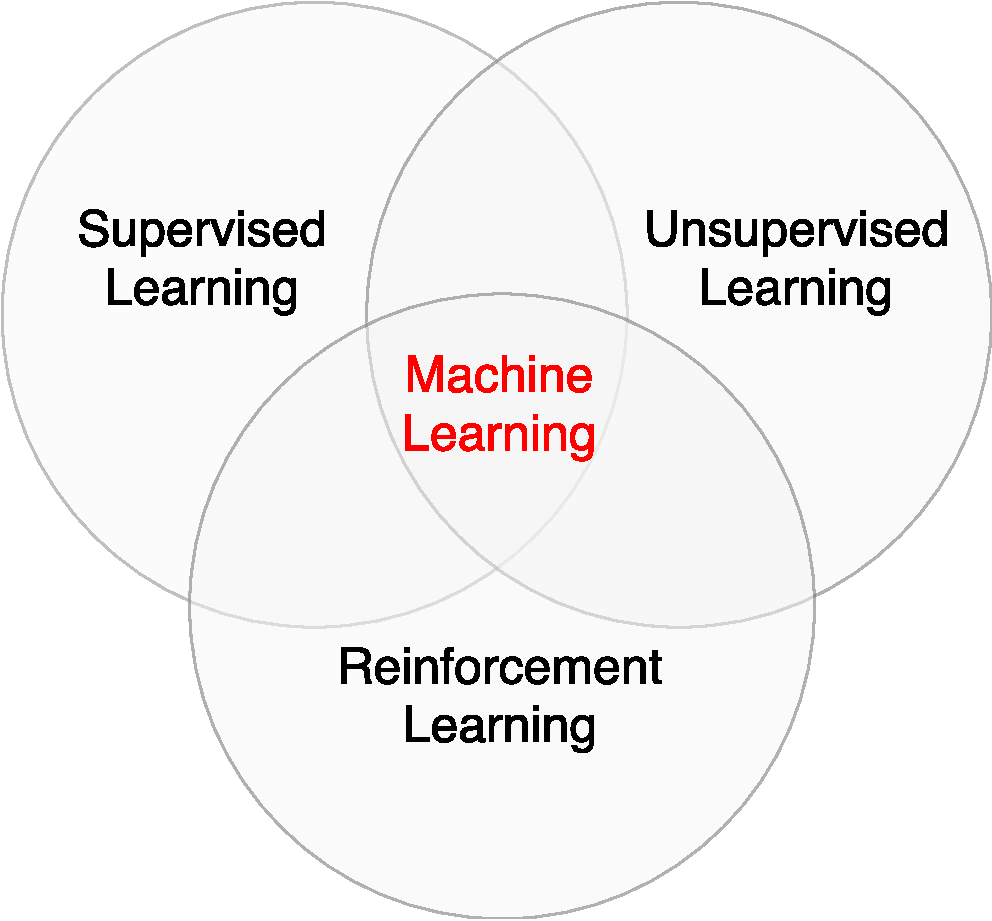
\includegraphics[width=0.7\textwidth]{Figures/RLandML}
	\caption{Reinforcement Learning and Machine Learning}
	\label{fig:RLandML}
\end{figure}
Reinforcement learning considers the problem of planning in real time decision making and the models for prediction related to planning. The interactive goal-directed agent is able to operate in an uncertain set up, make decisions despite uncertainty and predict future events. The agent is not necessarily a robot; it can be any component in a larger system in which it interacts directly with the system and indirectly with the system’s environment. The environment is everything that the agent interacts with, it is the outer world.

There is a special concern in reinforcement learning which is not present in the other machine learning approaches. It is the issue of balancing exploitation of the knowledge that the agent has and exploration of new information in order to improve the current knowledge base.

A variety of different scientific fields intersect with reinforcement learning, especially mathematics, namely, statistics and optimization, which have an important background contribution to the reinforcement learning methods. “For example, the ability of some reinforcement learning methods to learn with parameterized approximators addresses the classical “curse of dimensionality” in operations research and control theory” \cite{Sutton}. The relationship between reinforcement learning and optimization can be exemplified by the idea of maximization of the reward signal. Actually, in reinforcement learning the agent intends to maximize the reward, but not necessarily achieves the maximum. Reinforcement learning is also part of the engineering and computer science subjects. The related algorithms have a close resemblance to the biological brain systems of animals and humans due to the reward factor involved, therefore it also binds with the psychology and neuroscience fields. The diagram in \Cref{fig:RLandOther} illustrates how reinforcement learning relates to other scientific disciplines.
\begin{figure}[H]
	\centering
	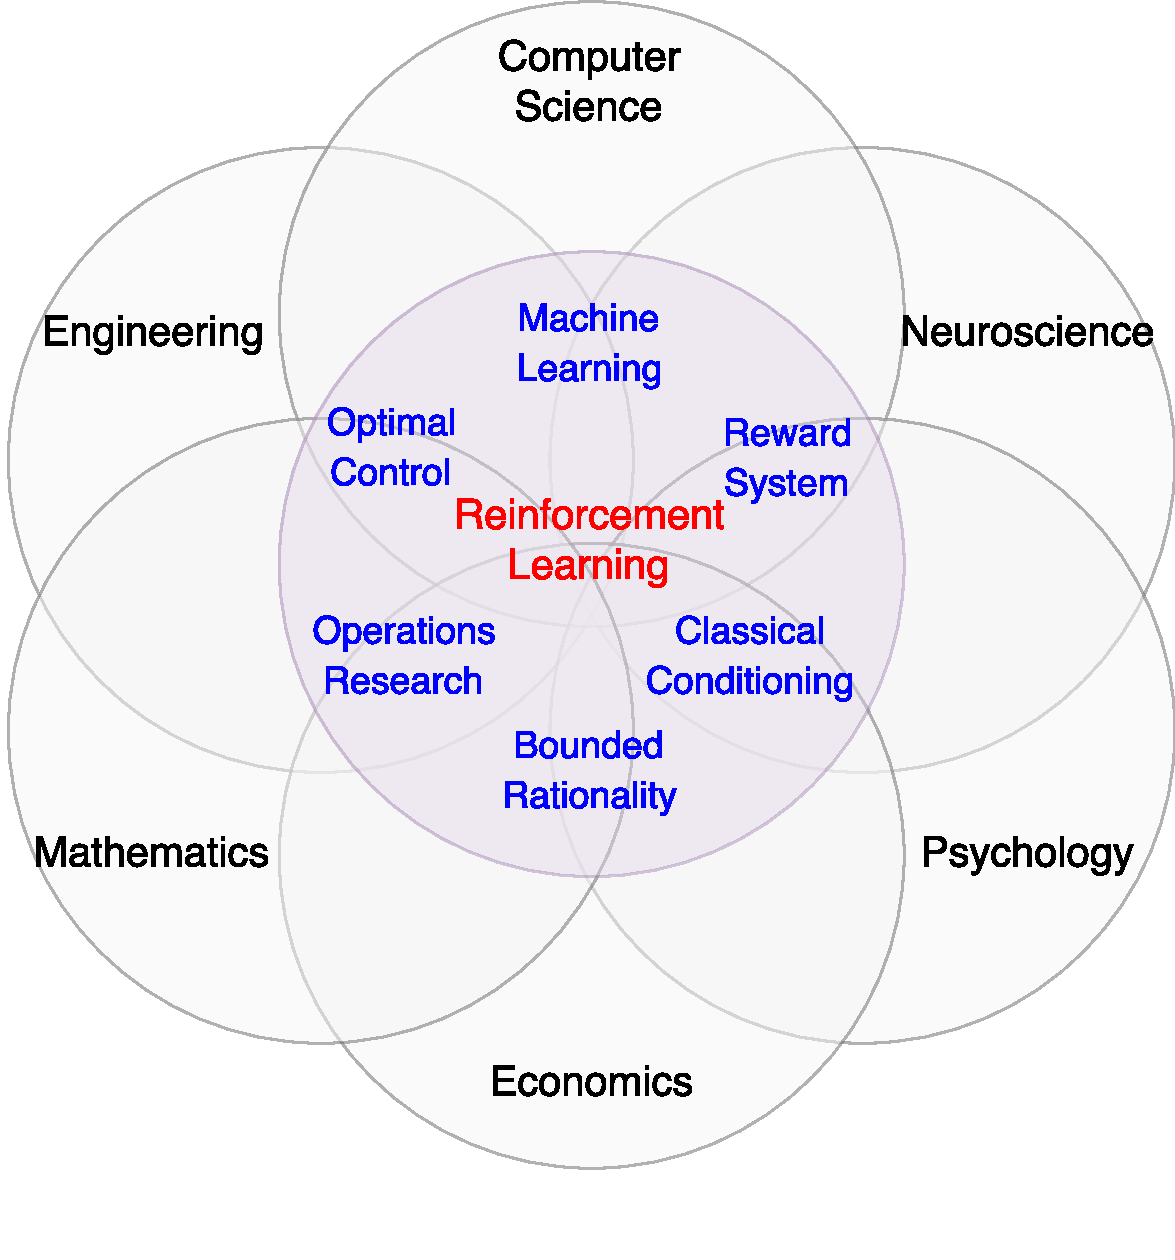
\includegraphics[width=0.7\textwidth]{Figures/RLandOther}
	\caption{Reinforcement Learning and other disciplines}
	\label{fig:RLandOther}
\end{figure}
\subsection{Elements of an RL problem}
A reinforcement learning problem contains at least one of the elements: reward signal, value function, policy, environment model.

The reward signal represents a feedback from the environment as a response to the agent’s behavior in that environment, therefore the agent cannot change the feedback that it receives, but it can behave accordingly so as to maximize the gained reward signals during its lifetime. The “reward signal defines the goal in a reinforcement learning problem” \cite{Sutton}. It serves as a problem definition and as a basis for modifying the policy.

The policy maps states to actions, so that when the agent is in a specific state, it chooses an action based on the defined policy. A policy is enough to describe the behavior of the agent and therefore, it is the core of reinforcement learning.

The value function provides values for judging about the quality of a state based on the estimated maximum reward it can yield in the long run, in contrast with the reward which expresses only the immediate advantage of being in a specific state.

The model is a representation of the environment’s behavior. In a model-free reinforcement learning (trial-and-error) problem the agent cannot plan its future, because it doesn’t have a model basis, whereas in mode-based problems the agent can plan its future actions based on the environment’s modelled behavior and expected rewards in certain states.
\subsection{Markov Decision Processes in RL}
The general reinforcement learning problem formulation has the format of a finite MDP. The interaction between the agent and environment happens at each time step of a sequence of discrete time steps, $t=0,1,2,3,...$, where at each time step $t$ the agent receives a representation of the world - a state, $S_{t}\in S$, from a set of possible states $S$, selects an action $A_{t}$ from a set of possible actions $A(S_{t})$ for the state $S_{t}$ by implementing a policy $\pi_{t}$, where $\pi_{t}(a|s)$ is the probability that $A_{t}=a$ if $S_{t}=s$, and in the next time step $t+1$ the agent receives a reward signal $R_{t+1}\in R$ from the environment ending up in a new state $S_{t+1}$ \cite{Sutton}. The diagram in \Cref{fig:AgentEnv} illustrates the interaction between the agent and the environment.
\begin{figure}[H]
	\centering
	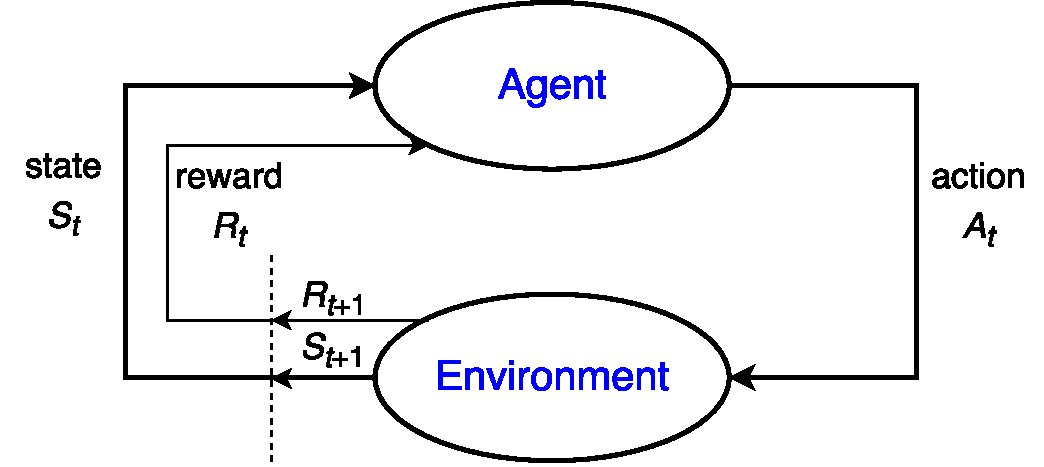
\includegraphics[width=0.7\textwidth]{Figures/Agent-EnvironmentInteraction}
	\caption{Agent - environment interaction}
	\label{fig:AgentEnv}
\end{figure}
Reinforcement learning methods provide ways to adjust the policy based on the accumulated experience with the goal of maximizing the total cumulative reward in mind. An example for representing the goal in a reinforcement learning problem like that of making a robot learn to walk would be by giving a reward on each time step proportional to the robot's forward motion. “The reward signal is your way of communicating to the robot \textit{what} you want it to achieve, not \textit{how} you want it achieved” \cite{Sutton}.

A formal definition of the cumulative reward received in the long run is expressed by the expected return $G_{t}$, which is a function of rewards sequence $R_{t+1},R_{t+2},...,R_{T}$ received after the time step $t$, where $T$ is the last time step. In order to express the return more conveniently the concept of \textit{discounting} is introduced, which determines the current value of the future rewards. The formula generalized for both episodic and continuing tasks is the following: 
\begin{equation}
G_{t}=R_{t+1}+\gamma R_{t+2}+\gamma ^2R_{t+3}+...=\sum_{k=0}^{T-t-1}\gamma ^kR_{t+k+1}, 
\end{equation}
where $\gamma$ is the discount rate, $0\leq \gamma\leq1$. In the case of episodic tasks where there is a terminal state after some time steps, $\gamma=1$. For the cases in which the process is continuous and the final step is infinite, $T=\infty$. 

With the discounting factor, the reward received after $k$ time steps has the value "$\gamma ^{k-1}$ times what it would be worth if it were received immediately" \cite{Sutton}. In the extreme point where $\gamma=0$, it is said that the agent is myopic, because it only maximizes over the immediate rewards and not the future rewards, whereas if $\gamma$ is closer to $1$ the agent is farsighted and sees far into the future considering the future rewards when picking actions.

The \textit{state} that has the Markov property represents all the useful information in order to make a sufficient statistic for the future. With Markov states we have the best possible basis for choosing action \cite{Sutton}. The environment's feedback at time step $t+1$ after a particular action was taken at time step $t$ depends on the events happened before. If the state has the Markov property instead, then the feedback of the environment depends only on that state, because that state represents all the previous events. In this case the one step environment dynamics of a finite MDP can be expressed by the following formula:
\begin{equation}\label{psrsa}
p(s',r|s,a)=Pr\left \{ S_{t+1}=s',R_{t+1}=r|S_{t}=s,A_{t}=a \right \}
\end{equation}
Based on the formula presented in (\ref{psrsa}) we can also compute the expected rewards for state-action pairs \cite{Sutton},
\begin{equation}
r(s,a)=\mathop{{}\mathbb{E}}\left [ R_{t+1}|S_{t}=s,A_{t}=a \right ]=\sum_{r\in R}r\sum_{s'\in S}p(s',r|s,a)
\end{equation}
the \textit{state-transition probabilities}
\begin{equation}
p(s'|s,a)=Pr\left \{ S_{t+1}=s'|S_{t}=s,A_{t}=a \right \}=\sum_{r\in R}p(s',r|s,a)
\end{equation}
and the expected rewards for state-action-next-state triples,
\begin{equation}
r(s,a,s')=\mathop{{}\mathbb{E}}\left [ R_{t+1}|S_{t}=s,A_{t}=a,S_{t+1}=s' \right ]=
\frac{\sum_{r\in R}rp(s',r|s,a)}{p(s'|s,a)}
\end{equation}
Value functions estimate how good it is to be in a specific state given the expected return and the policy.

The \textit{state-value function} for policy $\pi$, $v_{\pi }$ expresses the expected value of a random variable given the followed policy $\pi$ at any time step $t$:
\begin{equation}
v_{\pi }(s)=\mathop{{}\mathbb{E}_{\pi}}\left [G_{t}|S_{t}=s \right ]=\mathop{{}\mathbb{E}_{\pi}}\left [ \sum_{k=0}^{\infty}\gamma ^kR_{t+k+1} |S_{t}=s\right ]
\end{equation}

The \textit{action-value function} for policy $\pi$, $q_{\pi }$ is the value of taking an action $a$ in a state $s$ while following the policy $\pi$:
\begin{equation}
q_{\pi }(a,s)=\mathop{{}\mathbb{E}_{\pi}}\left [G_{t}|S_{t}=s,A_{t}=a \right ]=\mathop{{}\mathbb{E}_{\pi}}\left [ \sum_{k=0}^{\infty}\gamma ^kR_{t+k+1} |S_{t}=s,A_{t}=a\right ]
\end{equation}

Value functions have the property of being expressed recursively. The recursive representation is actually the \textit{Bellman equation} and it's solution is the value of $v_{\pi }$. It is like a look ahead procedure, where the value of a current state is evaluated by looking ahead at the values that future states can offer. "The Bellman equation averages over all the possibilities, weighting each by its probability of occurring. It states that the value of the start state must equal the (discounted) value of the expected next state, plus the reward expected along the way" \cite{Sutton}:
\begin{equation}\label{StateValueFunction}
v_{\pi }(s)=\mathop{{}\mathbb{E}_{\pi}}\left [G_{t}|S_{t}=s \right ]=\sum_{a}\pi(a|s)\sum_{s',r}p(s',r|s,a)\left [ r+\gamma v_{\pi }(s') \right ]), \forall s\in S
\end{equation}
The Bellman equation represents the basis of different ways of computing, approximating, and learning $v_{\pi }$ \cite{Sutton}.

In finite MDPs, an \textit{optimal policy} $\pi_{*}$ is the policy for which its expected return for all the states is greater than or equal to the expected return of all the other policies. There can be many policies that are optimal due to their \textit{state-value function}, which evaluates the same for all the optimal policies:\begin{equation}
v_{*}(s)=\max_{\pi}v_{\pi}(s), \forall s\in S
\end{equation}

Analogically, the \textit{optimal action-value function} is formed:
\begin{equation}
q_{*}(s,a)=\max_{\pi}q_{\pi}(s,a), \forall s\in S , a \in A(s)
\end{equation}

The \textit{Bellman optimality equation} for $v_{*}$ is the value of a state on the optimal policy basis, which is the same as the expected return of the best action for that state \cite{Sutton}:
\begin{equation}\label{BellmanOptimalityVstar}
\begin{split}
v_{*}(s)&=\max_{a \in A(s)}q_{\pi*}(s,a) \\
&=\mathop{{}\mathbb{E}}\left [ R_{t+1} + \gamma v_{*}(S_{t+1})|S_{t}=s, A_{t}=a  \right ] \\
&=\max_{a \in A(s)}\sum_{s',r}p(s',r|s,a)\left [ r+\gamma v_{*}(s') \right ]
\end{split}
\end{equation}

And the \textit{Bellman optimality equation} for $q_{*}$ is the following:
\begin{equation}\label{BellmanOptimalityQstar}
\begin{split}
q_{*}(s,a)&=\mathop{{}\mathbb{E}}\left [ R_{t+1} + \gamma \max_{a'}q_{*}(S_{t+1},a')|S_{t}=s, A_{t}=a  \right ] \\
&=\sum_{s',r}p(s',r|s,a)\left [ r+\gamma\max_{a'}q_{*}(s',a') \right ]
\end{split}
\end{equation}

The Bellman optimality equation generates a system of $N$ nonlinear equations, where $N$ is the number of states. It can be simply solved by applying some nonlinear methods when the system dynamics ($p(s',r|s,a)$) are known. The solution to the Bellman optimality equation helps in defining the optimal policy; e.g. one can, at any state, choose the action that corresponds to the maximum return, which is also valid in the long term, because the values take into account the reward consequences of all possible future behavior options \cite{Sutton}. In the case of the action-value pairs, if the system's dynamics are unknown, then the actions would still be optimal, because the agent would choose the actions that would maximize $q_{*}$.

\subsection{Insight into the Solution Methods of RL}
The solution methods for the reinforcement learning problem can be divided into two groups, \textit{tabular} and \textit{approximate}. The tabular solution methods find exact, optimal solutions and are more suitable when the states and actions space is rather small, while the approximate solution methods provide approximate solutions and it is applicable to large spaces problems.

The process of \textit{generalized policy iteration} (GPI) provides a good way of getting insight into the methods of RL. GPI employs a sequence of interleaved policy evaluations and policy improvements, where the given policy is evaluated, for example, by computing it's value function, and the policy is improved by using the value function. This process is proven to converge to an optimal policy and value function for the classical dynamic programming methods. GPI represents the way that almost all RL methods work. The \Cref{fig:GPI} illustrates the process better.
\begin{figure}[H]
	\centering
	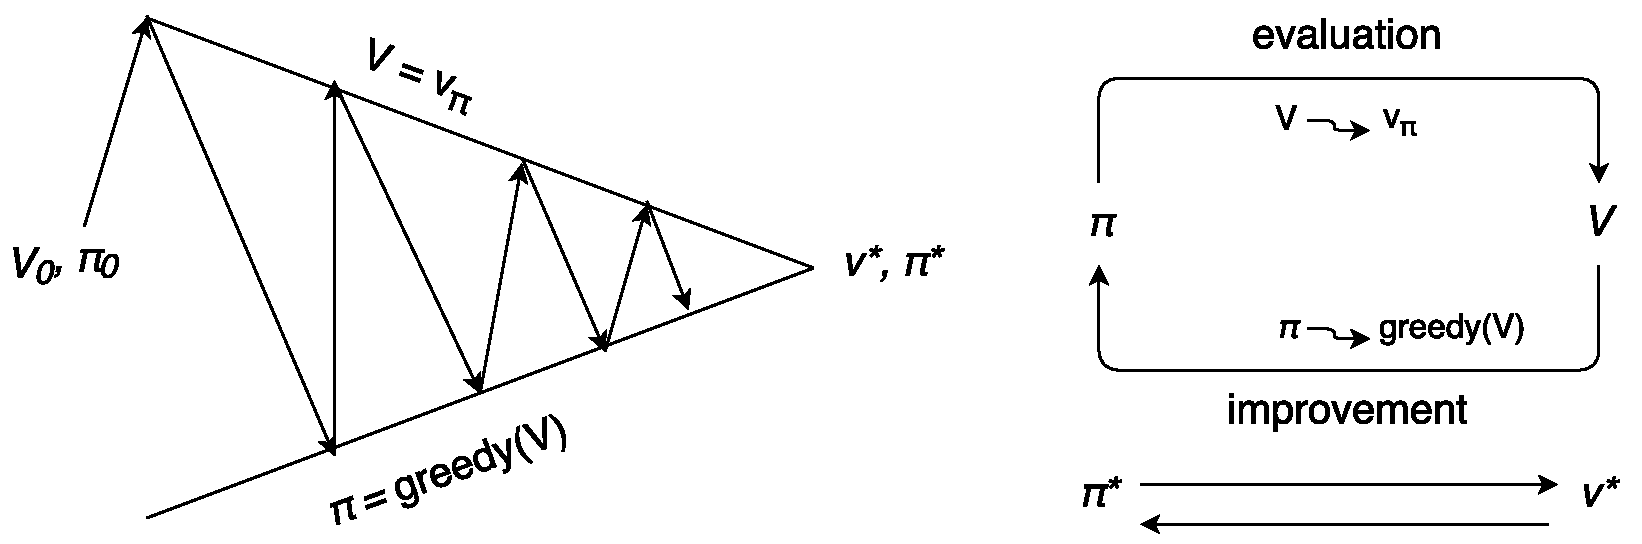
\includegraphics[width=0.9\textwidth]{Figures/GPI}
	\caption{Generalized Policy Iteration}
	\label{fig:GPI}
\end{figure}
Another way of presenting the GPI is in terms of \textit{prediction} and \textit{control}. The prediction problem is referring to policy evaluation or the estimation of $v_{\pi}$ for a given policy $\pi$, whereas the control problem is referring to the actual optimal policy $\pi_{*}$ seeking.

The relevant notions for describing the methods of RL are \textit{backup} and \textit{bootstrap}. A \textit{full backup} updates a state's value on the basis of the next states estimated values. \textit{Bootstrapping} refers to the idea of updating estimates based on other estimates.

Usually, the RL solution methods vary in the way they approach the prediction and control problems, and also in whether they need a model of the environment or they use bootstrapping.

\subsection{Tabular solution methods}
The tabular solution methods include three important classes of methods for solving the finite MDP: \textit{Dynamic Programming} (DP), \textit{Monte Carlo} (MC) and \textit{Temporal-Difference} (TD) learning. These methods will be generally presented in the following pages.

\subsubsection{Dynamic Programming}
Dynamic programming uses the Bellman optimality equations \ref{BellmanOptimalityVstar} and \ref{BellmanOptimalityQstar} as update functions for \textit{policy iteration}, which yields a sequence of monotonically increasing value functions and policies: ${\pi}_{0}\overset{E}{\rightarrow}v_{{\pi}_{0}}\overset{I}{\rightarrow}{\pi}_{1}\overset{E}{\rightarrow}v_{{\pi}_{1}}\overset{I}{\rightarrow}{\pi}_{2}\overset{E}{\rightarrow}...\overset{I}{\rightarrow}{\pi}_{*}\overset{E}{\rightarrow}v_{*}$, where $E$ stands for evaluation and $I$ - for improvement. That is, an arbitrary fixed policy is evaluated by computing it's state-value function and is improved by computing it's state-action value function. If the state-action value function of choosing an action $a \neq \pi(s)$ is greater than the state-value function $v_{\pi}(s)$, then the policy is changed to a new policy. The formula for getting a new policy is given by \ref{PolicyImprovement}:
\begin{equation}\label{PolicyImprovement}
\begin{split}
\pi'&=\arg\!\max_{a}q_{\pi}(s,a)\\
&=\arg\!\max_{a}\mathop{{}\mathbb{E}}\left [ R_{t+1} + \gamma v_{\pi}(S_{t+1})|S_{t}=s, A_{t}=a  \right ] \\
&=\arg\!\max_{a}\sum_{s',r}p(s',r|s,a)\left [ r+\gamma v_{\pi}(s') \right ]
\end{split}
\end{equation}

Unlike the DP methods, the Monte Carlo and the temporal-difference solution methods don't require the model parameters to be known in advance, meaning that no previous knowledge about the environment is needed and that the agent learns exclusively from it's \textit{experience} (sampled states, actions, rewards). The MC method doesn't bootstrap, whereas TD does use bootstrapping, like the DP methods.

\subsubsection{Monte Carlo}
Monte Carlo differs from DP in the way it handles the prediction problem. It uses averages over the sampled returns from a specific state on episode-by-episode basis in order to learn over multiple observed returns the value function, whereas in DP the value function was computed from the knowledge of the MDP. The policy evaluation is performed by computing the value of the state-action pairs for the visited states over an episode. The policy improvement is performed by adjusting the policy closer to the action with the maximal value for a specific state.

Because MC doesn't make all the possible actions, it is required to employ some kind of guarantee for exploration. This can be achieved by assigning nonzero probabilities for all the actions in order to make sure they are going to be picked eventually. This is called \textit{exploring starts}. A better approach are the \textit{on-policy} and \textit{off-policy} methods. 

On-policy methods have probabilities greater than zero for all their actions, meaning that they have \textit{soft} policies. The policies in on-policy methods become closer to an optimal deterministic policy in time. The exploring starts is an example of on-policy method. Another example would be an $\epsilon$-greedy policy where the best action is chosen with the probability $1-\epsilon$ and, sometimes, another random action is chosen with the probability $\epsilon$.

Off-policy methods use 2 policies: a \textit{target policy} $\pi$, which is a deterministic policy, like the one presented in the on-policy methods, and a \textit{behavior policy} $\mu$, which is stochastic in states and generates data by exploring. Both policies have non zero probabilities that ensures the coverage property. Off-policy methods can be implemented with \textit{importance sampling} technique. The importance sampling technique computes an importance sampling ratio based on the relative probabilities of the returns' trajectories from both policies and it is used for weighting the returns for learning the value function.

\subsubsection{Temporal Difference}
Temporal Difference differs from DP also in the way it handles the prediction problem. TD makes an estimate of the value function after each time step by sampling expected values and using current value estimates. Therefore, TD is a combination of MC sampling and DP bootstrapping. The simplest TD method is also called \textit{TD(0)}. The update function for TD(0) \ref{PolicyEvaluationTD0} is the following:
\begin{equation}\label{PolicyEvaluationTD0}
V(S_{t})\leftarrow V(S_{t})+\alpha \left [ R_{t+1}+\gamma V(S_{t+1})-V(S_{t}) \right ]
\end{equation}
If we compare the MC target with the TD target, the MC target has $G_{t}$ instead of the immediate reward and the value estimate of the next state. The square brackets represents the TD error, or the MC error in the MC update function. An important observation is that the sum of the time steps TD errors gives an episode of MC error.

For solving the control problem with TD(0) and on-policy methods, action-value functions are used instead of the value function that we've just seen. A "transition from one action-state pair to another" \cite{Sutton} yields a quintuple of the form $(S_{t}, A_{t}, R_{t+1}, S_{t+1}, A_{t+1})$, \textit{Sarsa}, which is the name of the algorithm. Therefore, for evaluating the policy, an estimation of the $q_{\pi}$ is required and for improving the policy, $\pi$ is greedily adjusted closer to it's $q_{\pi}$.

An notable off-policy TD(0) algorithm is \textit{Q-learning}. It is an off-policy method because it learns the optimal action-value function $q_{\pi*}$ independent of the policy. The action is picked greedily according to the estimated $Q$ but the $Q$ is updated based on the action that produces maximal value. 

A slight change into the update function of $Q$ would lead us to the \textit{Expected Sarsa} algorithm. The change is that instead of maximizing over the next action-value pairs, the expected return is taken, which considers the probabilities of making those actions according to the current policy. Expected Sarsa is a better algorithm in comparison with Sarsa and Q-learning.

The MC and TD methods are extended into more complicated and powerful forms to achieve better performance, but the essence of these methods perpetuates in all the other algorithms. An idea about combining these two methods would be to unify them under \textit{n-step} algorithms instead of the extreme one time step in TD(0) and a whole episode in MC, or perform additions of other features like eligibility traces and model learning.
	
\subsection{Approximate solution methods}
The approximate solution methods are an extension to the tabular solution methods for huge states spaces problems. In this type of problems, the goal is to find a good approximate solution under the condition of restricted computational resources. Because almost every visited state is seen for the first time, every state being so unique, the agent needs to be able to make sense of it and, therefore, usefully generalize the information it gets. This is possible thanks to function approximation. “Function approximation is an instance of supervised learning, the primary topic studied in machine learning, artificial neural networks, pattern recognition, and statistical curve fitting” \cite{Sutton}.

The value function is represented by a function of a weights vector instead of a table. The approximated value function looks like $\hat{v}(s,\theta)\approx v_{\pi}(s)$, which can be translated into words as the approximated value of a state $s$ given the weights vector $\theta$. The value function can be an artificial neural network with multiple layers where the weights are adjusted and learned. A single adjustment of the weights would change the value appreciation for all the states. This process is difficult to follow and track, but it is more powerful. This would create the necessary \textit{generalization} for the agent to learn from it and apply knowledge in multiple similar, but different states.

With function approximation different supervised machine learning methods can be applied to simulate outputs for a set of inputs. The estimated value of a state $s$ should look more like a number $g$ and this relation $s \mapsto g$ can be used as a training example for supervised learning that would learn to predict values for other states. $s \mapsto g$ is referred to as a back-up, where $s$ is the state backed-up and $g$ is the backed-up value or target. For example, the target in MC methods is the return $G_{t}$, so the back-up is $S_{t} \mapsto G_{t}$, whereas the back-up in TD(0) is $S_{t} \mapsto R_{t+1}+\gamma\hat{v}(S_{t+1}, \theta_{t}) $.

Some common way of doing function approximation is based on gradient principles. For any $\theta$ the function approximator can not exactly represent all the states and examples, therefore the idea is to find a balance - a weights vector that would, as close as possible, represent all the states. A performance measure could be defined by the \textit{mean squared value error} (MSVE) shown below (\Cref{MSVE}). The error represents the squared difference between the estimated value $\hat{v}(s,\theta)$ and the actual value $v_{\pi}(s)$, whereas the $d(s)$ represents the weight or the distribution of the error for a state $s$. The goal would become the minimization of MVSE.
\begin{equation}\label{MSVE}
MVSE(\theta)=\sum_{s\in S} d(s) \left [ v_{\pi}(s) - \hat{v}(s,\theta) \right ]^{2}
\end{equation}

For each training example the \textit{Stochastic Gradient Descent} (SGD) method would update the weights so that they minimize the error in that example:
\begin{equation}\label{SGD}
\theta_{t+1}=\theta_{t}+\alpha \left [ v_{\pi}(S_{t}) - \hat{v}(S_{t},\theta_{t}) \right ]\nabla\hat{v}(S_{t},\theta_{t})
\end{equation}
In the MC method, the target is an unbiased estimate of $v_{\pi}(s)$, therefore the SGD would be a good choice to be applied, because it would converge to a locally optimal solution for the value function. In the bootstrapping cases, however, SGD is not the best choice, because the targets usually depend on the weights vector that is changing and causing the targets to be biased. These methods are called \textit{semi-gradient} methods instead, and they converge in the linear case.

Linear methods have feature vectors $\phi(s)$ that represent the state. The inner product between the feature vector $\phi(s)$ and the weights $\theta$ makes up the function approximation $v_{\pi}(s,\theta)$. In such a situation the SGD method can be applied and get an even simpler form of weights update. This is proven to converge to a global optimum, including for the MC linear function approximation version and the semi-gradient TD(0) with an additional theorem.

\subsubsection{Artificial Neural Networks}
Nonlinear methods for function approximation involve \textit{artificial neural networks} (ANNs). ANNs are the product of inspiration from the neural networks in the brains of animals and humans. Their properties and functionality have been successfully replicated in ANNs. An ANN is a layered structure of neurons which has minimum one input layer and one output layer. Each layer has a number of units (neurons) that are connected to the units in another layer. The connections are assigned weights that are used for the unit's \textit{activation}. In order to perform activation, a weighted sum of it's inputs is computed at each unit and then passed to an activation function to produce output. There are different activation functions, though, and the choice depends on the type of problem.

In dependence of the structure of the network, there are different types of ANNs. For example, a simple case of \textit{feedforward} ANN without any loops, with an input layer of 4 units, 2 hidden layers, and an output layer with 2 units is presented in the \Cref{fig:feedforward}:
\begin{figure}[H]
	\centering
	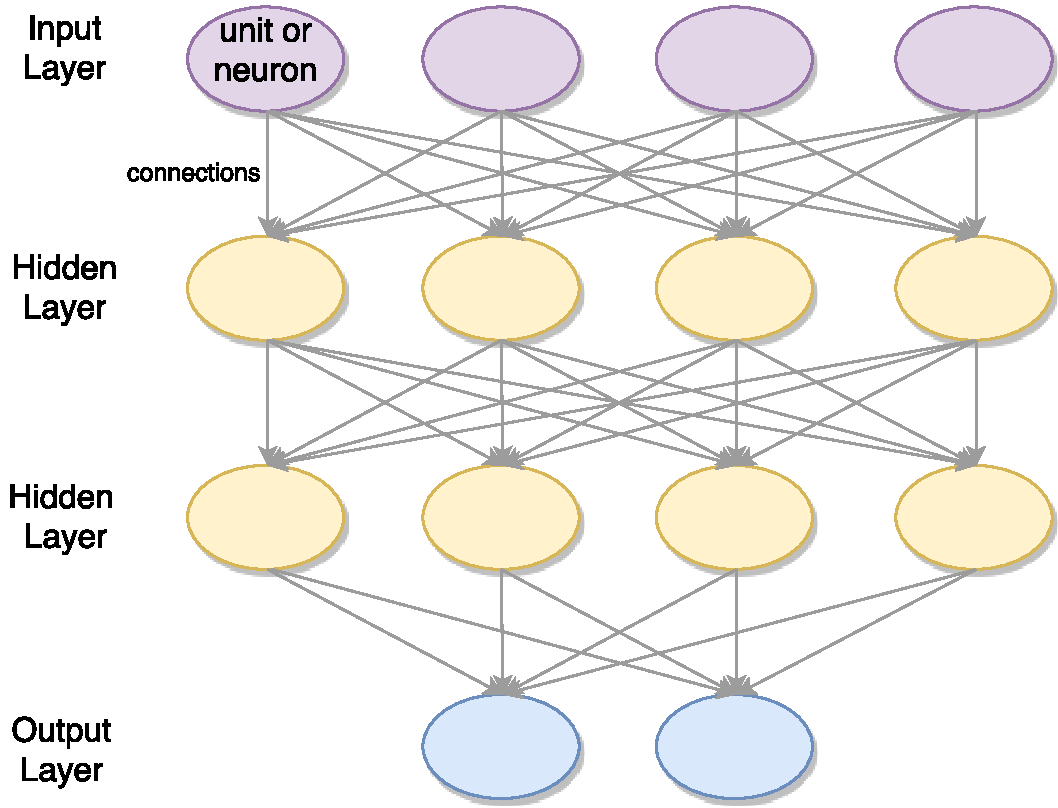
\includegraphics[width=0.7\textwidth]{Figures/Feedforward}
	\caption{Feedforward ANN}
	\label{fig:feedforward}
\end{figure}
Some ANNs can be called \textit{deep}. This qualifier describes the networks that have many hidden layers, precisely more than two. More hidden layers would compute more abstract representations of the input data, which means richer features. Deep ANNs are harder to train, but they are more powerful, and are especially used in modern artificial intelligence applications.

Usually, ANNs learn by a SGD method. More precisely, learning implies the definition of an objective function that describes the performance of the network, and, which is either minimized or maximized. An objective function can be the loss of the network over a set of training examples. In RL, an ANN can use TD errors in computing the loss function and learning the value function, or maximize the reward, or use a policy-gradient algorithm \cite{Sutton}. No matter the case, the partial derivatives are required to determine the influence of a weight change on the network's performance, and they can be obtained with the help of the gradient.

In order to find the gradient, an ANN can use the back-propagation algorithm. In the forward pass, the network's units would compute the outputs, whereas in the backward pass - the partial derivatives with respect to each weight. However, the back-propagation algorithm isn't that efficient for the deep ANNs, because of the overfitting problem.

A special structure of the network's architecture, like that of the deep \textit{convolutional networks} (CNN) would make it possible to use the back-propagation algorithm in deep ANNs, too. CNN is a very important type of ANN that is especially used for finding spatially correlated patterns in images while sharing weights and excluding the need of full connectivity between units.

\textit{Recurrent neural networks} (RNN)

\subsubsection{Policy Gradient Methods}
The \textit{Policy Gradient Methods} learn a \textit{parameterized policy} and makes it possible to select the action without calculating the value function. So, in a given state $s$, at a given time $t$, the agent selects an action $a$ based on the weights vector ${\theta}$ of the policy: ${\pi}(a|s,{\theta})=Pr\{A_{t}=a|S_{t}=s,{\theta}_{t}={\theta}\}$. The policy weights are learned according to an approximate gradient of a performance indicator ${\eta}({\theta})$ with respect to the policy weights, which tries to maximize the performance. All the methods of the form \Cref{gradM} are policy gradient methods:
\begin{equation}\label{gradM}
\theta_{t+1}=\theta_{t}+\alpha \nabla \eta (\theta_{t})
\end{equation}
The policy gradient methods are suitable for both \textit{discrete} and \textit{continuous} action spaces. For the discrete action space problems parameterized numerical preferences can be formed for each state-action pair, $h(s,a,\theta)$ \cite{Sutton}. The most preferred actions in each state have the highest probability of getting selected. The preferences can be parameterized randomly, for example, by being computed by a deep Q-network. The policy gradient theorem provides a formula for computing the gradient of the performance measure $\eta$ with respect to the policy weights vector $\theta$, composed of the state distribution $d_{\pi}(s)$, the state-action value function $q_{\pi}(s,a)$, and the gradient of the policy $\nabla_{\theta}\pi(a|s,\theta)$:
\begin{equation}\label{gradMTheorem}
\nabla\eta(\theta)=\sum_{a}d_{\pi}(s)\sum_{a}q_{\pi}(s,a)\nabla_{\theta}\pi(a|s,\theta)
\end{equation}

The methods that use both policy and value approximations are named \textit{actor-critic} methods, where the \textit{actor} estimates the policy weights vector for choosing an action and the \textit{critic} estimates the value weights for providing the information about the quality of a state the agent ends up in after making the action according to the policy. So, the actor is about the learned policy, and the critic - about the learned value function.
\section{Solution Methods of RL}\label{Solution Methods}
The solution methods for the reinforcement learning problem can be divided into two groups, \textit{tabular} and \textit{approximate}. The tabular solution methods find exact, optimal solutions and are more suitable when the states and actions space is rather small, while the approximate solution methods provide approximate solutions and it is applicable to large spaces problems.

The process of \textit{generalized policy iteration} (GPI) provides a good way of getting insight into the methods of RL. GPI employs a sequence of interleaved policy evaluations and policy improvements, where the given policy is evaluated, for example, by computing its value function, and the policy is improved by using the value function. This process is proven to converge to an optimal policy and value function for the classical dynamic programming methods. GPI represents the way that almost all RL methods work. The \Cref{fig:GPI} illustrates the process better.
\begin{figure}[H]
	\centering
	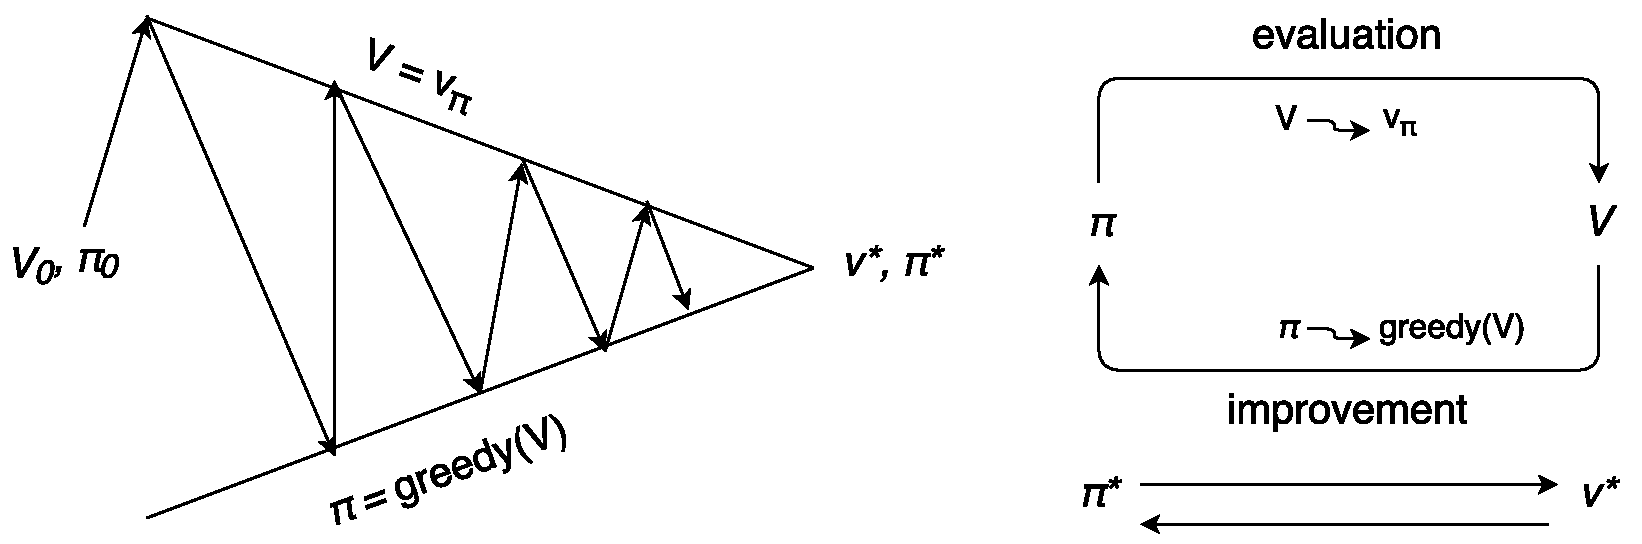
\includegraphics[width=0.9\textwidth]{Figures/GPI}
	\caption{Generalized Policy Iteration}
	\label{fig:GPI}
\end{figure}
Another way of presenting the GPI is in terms of \textit{prediction} and \textit{control}. The prediction problem is referring to policy evaluation or the estimation of $v_{\pi}$ for a given policy $\pi$, whereas the control problem is referring to the actual optimal policy $\pi_{*}$ seeking.

The relevant notions for describing the methods of RL are \textit{backup} and \textit{bootstrap}. A \textit{full backup} updates a state's value on the basis of the next states estimated values. \textit{Bootstrapping} refers to the idea of updating estimates based on other estimates.

Usually, the RL solution methods vary in the way they approach the prediction and control problems, and also in whether they need a model of the environment or they use bootstrapping.

\subsection{Tabular Solution Methods}
The tabular solution methods include three important classes of methods for solving the finite MDP: \textit{Dynamic Programming} (DP), \textit{Monte Carlo} (MC) and \textit{Temporal-Difference} (TD) learning. These methods will be generally presented in the following pages.

\subsubsection{Dynamic Programming}
Dynamic programming uses the Bellman optimality equations \ref{BellmanOptimalityVstar} and \ref{BellmanOptimalityQstar} as update functions for \textit{policy iteration}, which yields a sequence of monotonically increasing value functions and policies: ${\pi}_{0}\overset{E}{\rightarrow}v_{{\pi}_{0}}\overset{I}{\rightarrow}{\pi}_{1}\overset{E}{\rightarrow}v_{{\pi}_{1}}\overset{I}{\rightarrow}{\pi}_{2}\overset{E}{\rightarrow}...\overset{I}{\rightarrow}{\pi}_{*}\overset{E}{\rightarrow}v_{*}$, where $E$ stands for evaluation and $I$ - for improvement. That is, an arbitrary fixed policy is evaluated by computing it's state-value function and is improved by computing it's state-action value function. If the state-action value function of choosing an action $a \neq \pi(s)$ is greater than the state-value function $v_{\pi}(s)$, then the policy is changed to a new policy. The formula for getting a new policy is given by \ref{PolicyImprovement}:
\begin{equation}\label{PolicyImprovement}
\begin{split}
\pi'&=\arg\!\max_{a}q_{\pi}(s,a)\\
&=\arg\!\max_{a}\mathop{{}\mathbb{E}}\left [ R_{t+1} + \gamma v_{\pi}(S_{t+1})|S_{t}=s, A_{t}=a  \right ] \\
&=\arg\!\max_{a}\sum_{s',r}p(s',r|s,a)\left [ r+\gamma v_{\pi}(s') \right ]
\end{split}
\end{equation}

Unlike the DP methods, the Monte Carlo and the temporal-difference solution methods don't require the model parameters to be known in advance, meaning that no previous knowledge about the environment is needed and that the agent learns exclusively from its \textit{experience} (sampled states, actions, rewards). The MC method doesn't bootstrap, whereas TD does use bootstrapping, like the DP methods.

\subsubsection{Monte Carlo}
Monte Carlo differs from DP in the way it handles the prediction problem. It uses averages over the sampled returns from a specific state on an episode-by-episode basis in order to learn the value function over multiple observed returns, whereas in DP the value function was computed from the knowledge of the MDP. The policy evaluation is performed by computing the value of the state-action pairs for the visited states over an episode. The return that is only known after an episode is used as a target for the value estimate of that state. The update formula for the value $v_{\pi}$ of a state following policy $\pi$ in a simple every-visit Monte Carlo method is:
\begin{equation}\label{PolicyEvaluationMC}
V(S_{t})\leftarrow V(S_{t})+\alpha \left [ G_{t}-V(S_{t}) \right ],
\end{equation}
where $\alpha$ is the step-size constant, $G_{t}$ is the actual return or also \textit{target}. The content between the square brackets is also called MC error.

The policy improvement is performed by adjusting the policy closer to the action with the maximal value for a specific state.

Because MC doesn't make all the possible actions, it is required to employ some kind of guarantee for exploration. This can be achieved by assigning nonzero probabilities for all the actions in order to make sure they are going to be picked eventually. This is called \textit{exploring starts}. A better approach are the \textit{on-policy} and \textit{off-policy} methods. 

On-policy methods have probabilities greater than zero for all their actions, meaning that they have \textit{soft} policies. The policies of on-policy methods become closer to an optimal deterministic policy in time. The exploring starts is an example of an on-policy method. Another example would be an $\epsilon$-greedy policy where the best action is chosen with the probability $1-\epsilon$ and, sometimes, another random action is chosen with the probability $\epsilon$.

Off-policy methods use 2 policies: a \textit{target policy} $\pi$, which is a deterministic policy, like the one presented in the on-policy methods, and a \textit{behavior policy} $\mu$, which is stochastic in states and generates data by exploring. Both policies have non-zero probabilities that ensure the coverage property. Off-policy methods can be implemented with \textit{importance sampling} technique. The importance sampling technique computes an importance sampling ratio based on the relative probabilities of the returns' trajectories from both policies and it is used for weighting the returns for learning the value function.

\subsubsection{Temporal Difference}\label{Temporal Difference}
Temporal Difference differs from DP also in the way it handles the prediction problem. TD makes an estimate of the value function after each time step by sampling expected values and using current value estimates. Therefore, TD is a combination of MC sampling and DP bootstrapping. The simplest TD method is also called \textit{TD(0)}. The update function for TD(0) \ref{PolicyEvaluationTD0} is the following:
\begin{equation}\label{PolicyEvaluationTD0}
V(S_{t})\leftarrow V(S_{t})+\alpha \left [ R_{t+1}+\gamma V(S_{t+1})-V(S_{t}) \right ]
\end{equation}

If we compare the MC target with the TD target, the MC target has $G_{t}$ instead of the immediate reward $R_{t+1}$ and the value estimate of the next state $V(S_{t+1}$. The square brackets represent the TD error or the MC error in the MC update function. An important observation is that the sum of the time steps TD errors gives an episode of MC error, because the TD(0) is a step-by-step algorithm, whereas MC is an episode-by-episode algorithm. The proof can be found in \cite{Sutton}.

For solving the control problem with TD(0) and on-policy methods, action-value functions are used instead of the value function that we've just seen. A "transition from one action-state pair to another" \cite{Sutton} yields a quintuple of the form $(S_{t}, A_{t}, R_{t+1}, S_{t+1}, A_{t+1})$, \textit{Sarsa}, which is the name of the algorithm. Therefore, for evaluating the policy, an estimation of the $q_{\pi}$ is required and for improving the policy, $\pi$ is greedily adjusted closer to it's $q_{\pi}$. The Sarsa update formula for Q is the following:
\begin{equation}\label{Sarsa}
Q(S_{t}, A_{t})\leftarrow Q(S_{t}, A_{t})+\alpha \left [ R_{t+1}+\gamma Q(S_{t+1}, A_{t+1})-Q(S_{t}, A_{t}) \right ]
\end{equation}

An notable off-policy TD(0) algorithm is \textit{Q-learning}. It is an off-policy method because it learns the optimal action-value function $q_{\pi*}$ independent of the policy. The action is picked greedily according to the estimated $Q$, but the $Q$ is updated based on the action that produces maximal value. The update formula for the Q-learning is the following:
\begin{equation}\label{Qlearning}
Q(S_{t}, A_{t})\leftarrow Q(S_{t}, A_{t})+\alpha \left [ R_{t+1}+\gamma \underset{a}{\textup{max}} Q(S_{t+1}, a)-Q(S_{t}, A_{t}) \right ]
\end{equation}

A slight change into the update function of $Q$ would lead us to the \textit{Expected Sarsa} algorithm. The change is that instead of maximizing over the next action-value pairs, the expected return is taken, which considers the probabilities of making those actions according to the current policy. Expected Sarsa is a better algorithm in comparison with Sarsa and Q-learning. The update formula for Expected Sarsa is the following:
\begin{equation}\label{ESarsa}
Q(S_{t}, A_{t})\leftarrow Q(S_{t}, A_{t})+\alpha \left [ R_{t+1}+ \gamma \sum_{a}\pi(a|S_{t+1}) Q(S_{t+1}, a)-Q(S_{t}, A_{t}) \right ]
\end{equation}

The Figure \ref{fig:BackupDiagrams} provides a summary of the tabular solution methods. It illustrates the backup diagrams for the different algorithms recently explored. The white circle represents a state, and the black circle - an action.
\begin{figure}[H]
	\centering
	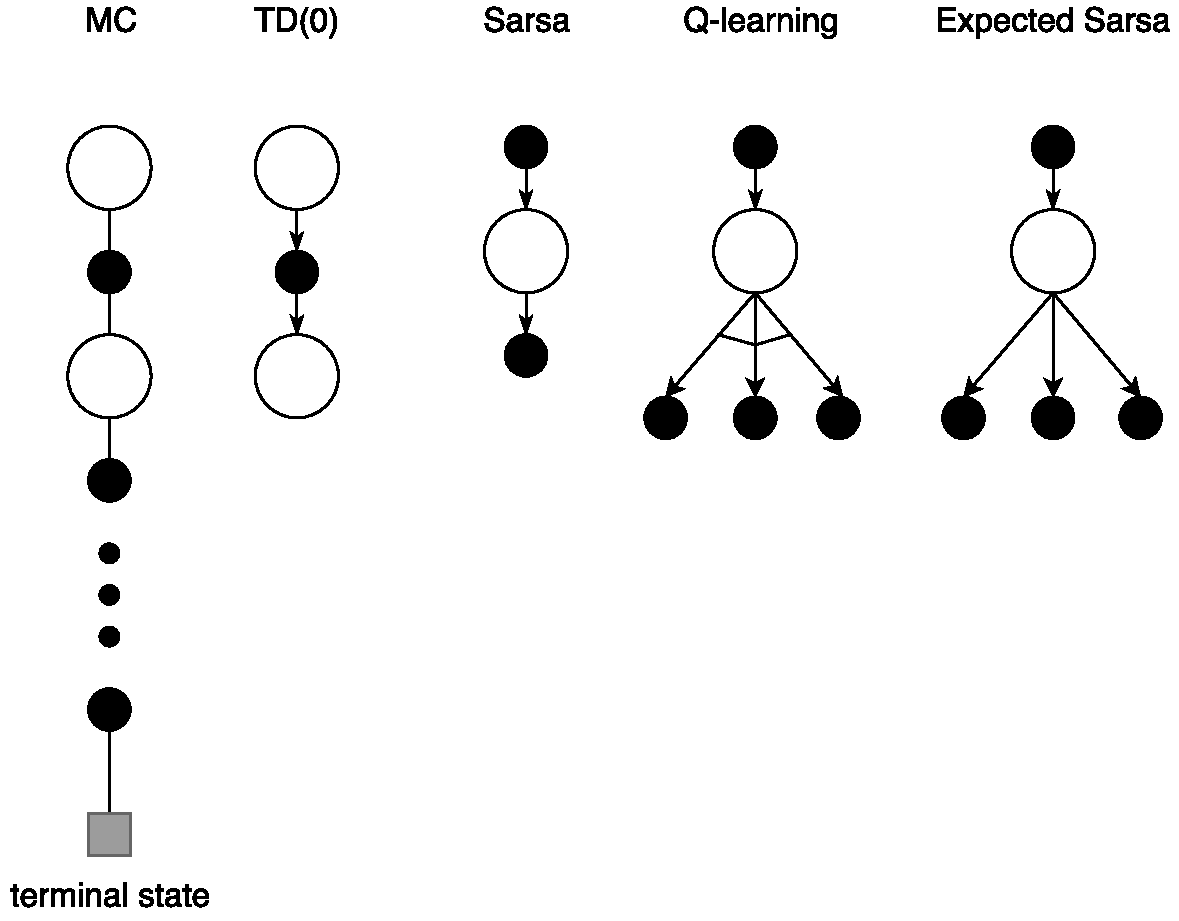
\includegraphics[width=0.7\textwidth]{Figures/BackupDiagrams}
	\caption{The backup diagrams of MC, TD(0), Sarsa, Q-learning, and Expected Sarsa}
	\label{fig:BackupDiagrams}
\end{figure}

The MC and TD methods are extended to more complicated and powerful forms to achieve better performance, but the essence of these methods perpetuates in all the other algorithms. An idea about combining these two methods would be to unify them under \textit{n-step} algorithms instead of the extreme one time step in TD(0) and a whole episode in MC or perform additions of other features like eligibility traces and model learning.
	
\subsection{Approximate Solution Methods}\label{Approximate solution methods}
The approximate solution methods are an extension to the tabular solution methods for huge states spaces problems. In this type of problems, the goal is to find a good approximate solution under the condition of restricted computational resources. Because almost every visited state is seen for the first time, every state being so unique, the agent needs to be able to make sense of it and, therefore, usefully generalize the information it gets. This is possible thanks to function approximation. “Function approximation is an instance of supervised learning, the primary topic studied in machine learning, artificial neural networks, pattern recognition, and statistical curve fitting” \cite{Sutton}.

The value function is represented by a function of a weights vector instead of a table. The approximated value function looks like $\hat{v}(s,\theta)\approx v_{\pi}(s)$, which can be translated into words as the approximated value of a state $s$ given the weights vector $\theta$. The value function can be an artificial neural network with multiple layers where the weights are adjusted and learned. A single adjustment of the weights would change the value appreciation for all the states. This process is difficult to follow and track, but it is more powerful. This would create the necessary \textit{generalization} for the agent to learn from it and apply knowledge in multiple similar, but different states.

With function approximation different supervised machine learning methods can be applied to simulate outputs for a set of inputs. The estimated value of a state $s$ should look more like a number $g$ and this relation $s \mapsto g$ can be used as a training example for supervised learning that would learn to predict values for other states. $s \mapsto g$ is referred to as a back-up, where $s$ is the state backed-up and $g$ is the backed-up value or target. For example, the target in MC methods is the return $G_{t}$, so the back-up is $S_{t} \mapsto G_{t}$, whereas the back-up in TD(0) is $S_{t} \mapsto R_{t+1}+\gamma\hat{v}(S_{t+1}, \theta_{t}) $.

Some common way of doing function approximation is based on gradient principles. For any $\theta$ the function approximator can not exactly represent all the states and examples, therefore the idea is to find a balance - a weights vector that would, as close as possible, represent all the states. A performance measure could be defined by the \textit{mean squared value error} (MSVE) shown below in \Cref{MSVE}. The error represents the squared difference between the estimated value $\hat{v}(s,\theta)$ and the actual value $v_{\pi}(s)$, whereas the $d(s)$ represents the weight or the distribution of the error for a state $s$. The goal would become the minimization of MVSE.
\begin{equation}\label{MSVE}
MSVE(\theta)=\sum_{s\in S} d(s) \left [ v_{\pi}(s) - \hat{v}(s,\theta) \right ]^{2}
\end{equation}

For each training example the \textit{Stochastic Gradient Descent} (SGD) method would update the weights so that they minimize the error in that example:
\begin{equation}\label{SGD}
\theta_{t+1}=\theta_{t}+\alpha \left [ v_{\pi}(S_{t}) - \hat{v}(S_{t},\theta_{t}) \right ]\nabla\hat{v}(S_{t},\theta_{t})
\end{equation}
In the MC method, the target is an unbiased estimate of $v_{\pi}(s)$, therefore the SGD would be a good choice to be applied, because it would converge to a locally optimal solution for the value function. In the bootstrapping cases, however, SGD is not the best choice, because the targets usually depend on the weights vector that is changing and causing the targets to be biased. These methods are called \textit{semi-gradient} methods instead, and they converge in the linear case.

Linear methods have feature vectors $\phi(s)$ that represent the state. The inner product between the feature vector $\phi(s)$ and the weights $\theta$ makes up the function approximation $v_{\pi}(s,\theta)$. In such a situation the SGD method can be applied and get an even simpler form of weights update. This is proven to converge to a global optimum, including for the MC linear function approximation version and the semi-gradient TD(0) with an additional theorem.

\subsubsection{Policy Gradient Methods} \label{PolicyGradMeths}
The \textit{Policy Gradient Methods} learn a \textit{parameterized policy} and makes it possible to select the action without calculating the value function. So, in a given state $s$, at a given time $t$, the agent selects an action $a$ based on the weights vector ${\theta}$ of the policy: ${\pi}(a|s,{\theta})=Pr\{A_{t}=a|S_{t}=s,{\theta}_{t}={\theta}\}$. The policy weights are learned according to an approximate gradient of a performance indicator ${\eta}({\theta})$ with respect to the policy weights, which tries to maximize the performance. All the methods of the form presented in \Cref{gradM} are policy gradient methods:
\begin{equation}\label{gradM}
\theta_{t+1}=\theta_{t}+\alpha \nabla \eta (\theta_{t})
\end{equation}

The policy gradient methods are suitable for both \textit{discrete} and \textit{continuous} action spaces. For the discrete action space problems, parameterized numerical preferences can be formed for each state-action pair, $h(s,a,\theta)$ \cite{Sutton}. The most preferred actions in each state have the highest probability of getting selected. The preferences can be parameterized randomly, for example, by being computed with a deep Q-network. 

The policy gradient theorem provides a formula for computing the gradient of the performance measure $\eta$ with respect to the policy weights vector $\theta$, composed of the state distribution $d_{\pi}(s)$, the state-action value function $q_{\pi}(s,a)$, and the gradient of the policy $\nabla_{\theta}\pi(a|s,\theta)$:
\begin{equation}\label{gradMTheorem}
\nabla\eta(\theta)=\sum_{a}d_{\pi}(s)\sum_{a}q_{\pi}(s,a)\nabla_{\theta}\pi(a|s,\theta)
\end{equation}

The methods that use both policy and value approximations are named \textit{actor-critic} methods, where the \textit{actor} estimates the policy weights vector for choosing an action and the \textit{critic} estimates the value weights for providing the information about the quality of a state the agent ends up in after making the action according to the policy. So, the actor is about the learned policy and the critic - about the learned value function. 

There is an algorithm which is called \textit{reinforce} and it also uses both policy and value function approximation, but it doesn't bootstrap. The critic, on the other hand, is a bootstrapping critic, which updates its states based on the value estimates of the next states. So, the initial reinforce algorithm has been changed for the actor-critic method: it's full return was replaced by one-step return. The one-step actor-critic algorithm is presented below \cite{Sutton}:
\begin{algorithm}[H]
	\caption{One-step Actor-Critic (episodic)}
	\label{algo:AC}
	\begin{algorithmic}
		\State Input: differentiable policy parameterization $\pi(a|s,\theta),\forall a\in A, s\in S,\theta\in\mathbb{R}^{n}$
		\State Input: differentiable state-value parameterization $\hat{v}(s,w),\forall s \in S, w \in \mathbb{R}_{m}$
		\State Parameters: $\alpha>0,\beta>0$
		\State Initialize policy weights $\theta$ and state-value weights $w$
		\Repeat
		\State Initialize $S$ (first state of episode)
		\State $I\leftarrow 1$
		\While{$S$ is not terminal}:
		\State $A\sim \pi(\cdot|S,\theta)$
		\State Take action $S$, observe $S'$, $R$
		\State $\delta\leftarrow R+\gamma\hat{v}(S',w)-\hat{v}(S,w)$ (if $S'$ is terminal, then $\hat{v}(S',w)=0$)
		\State $w\leftarrow w+\beta\delta\nabla_{w}\hat{v}(S,w)$
		\State $\theta\leftarrow \theta+\alpha I \delta\nabla_{\theta} \textup{log} \pi(A|S,\theta)$
		\State $I\leftarrow \gamma I$
		\State $S\leftarrow S'$
		\EndWhile
		\Until forever
	\end{algorithmic}
\end{algorithm}

As it was mentioned before, policy gradient methods work for discrete action spaces as well as for continuous. In the discrete actions problem, the policy is estimating the probability of each action in the discrete set. In the continuous actions space, on the other hand, the policy approximates the variance $\sigma^2$, and the mean $\mu$ of a normal distribution given by:
\begin{equation}\label{normalDistrib}
p(x)=\frac{1}{\sigma \sqrt{2\pi}}\textup{exp}(-\frac{(x-\mu)^2}{2\sigma ^2}),
\end{equation}
where $p(s)$ is the density of the probability at $x$. This is what makes the basis for the construction of a continuous policy, in which the weights-vector $\theta$ is included. The continuous policy formula is provided below:
\begin{equation}\label{continuousPolicy}
\pi(a|s,\theta)=\frac{1}{\sigma (s,\theta) \sqrt{2\pi}}\textup{exp}(-\frac{(a-\mu(s,\theta))^2}{2\sigma(s,\theta) ^2})
\end{equation}
The policy weights vector $\theta=[\theta_{\mu}, \theta_{\sigma}]^T$ is composed of two elements, $\theta_{\mu}$ and $\theta_{\sigma}$, that can be used further in function approximation algorithms. The form that these elements take is shown below:
\begin{equation}\label{mean}
\mu(s,\theta) = \theta_{\mu}^T\phi(s) \textup{    and    }
\sigma(s,\theta) = \textup{exp} (\theta_{\sigma}^T\phi(s)),
\end{equation}
where $\phi(s)$ is the feature vector, which can be, for example, the pixel values vector of an image.
\section{Artificial Neural Networks}\label{ANNsection}
Nonlinear methods for function approximation involve \textit{artificial neural networks} (ANNs). ANNs are the product of inspiration from the neural networks in the brains of animals and humans. Their properties and functionality have been successfully replicated in ANNs. An ANN is a layered structure of neurons which has minimum one input layer and one output layer. Each layer has a number of units (neurons) that are connected to the units in another layer. The connections are assigned weights that are used for the unit's \textit{activation}. In order to perform activation, a weighted sum of it's inputs is computed at each unit and then passed to an activation function to produce output. There are different activation functions, though, and the choice depends on the type of problem.

In dependence of the structure of the network, there are different types of ANNs. For example, a simple case of \textit{feedforward} ANN without any loops, with an input layer of 4 units, 2 hidden layers, and an output layer with 2 units is presented in the \Cref{fig:feedforward}:
\begin{figure}[H]
	\centering
	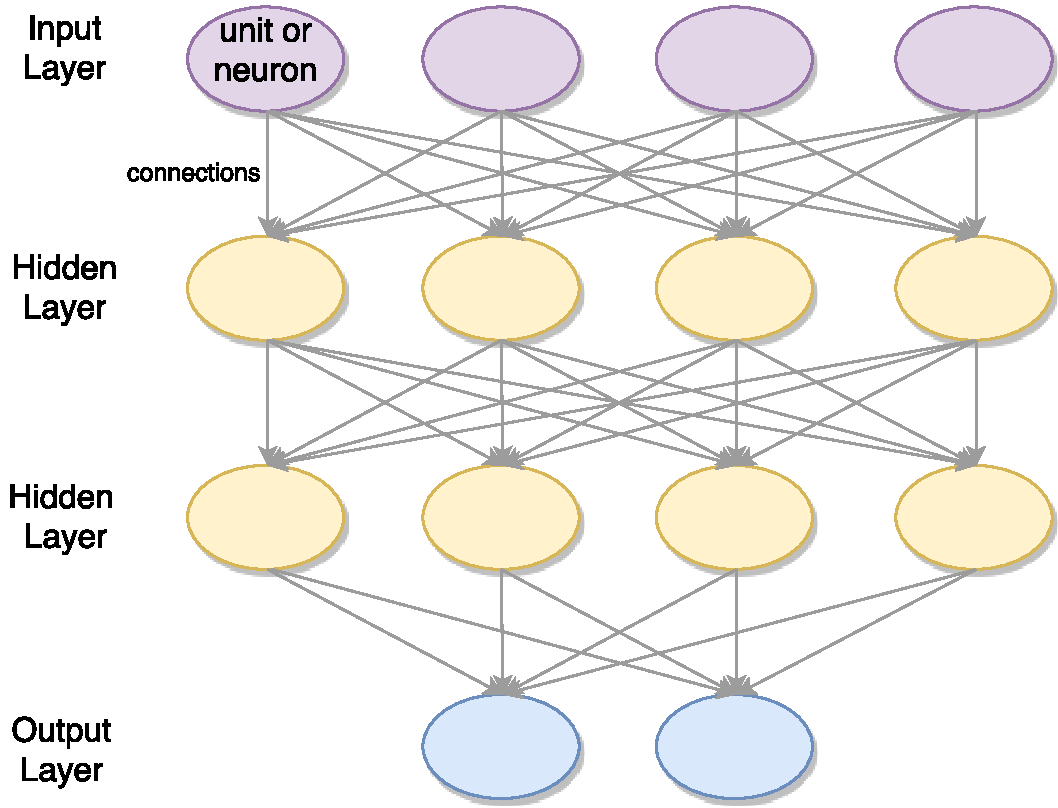
\includegraphics[width=0.7\textwidth]{Figures/Feedforward}
	\caption{Feedforward ANN}
	\label{fig:feedforward}
\end{figure}
Some ANNs can be called \textit{deep}. This qualifier describes the networks that have many hidden layers, precisely more than two. More hidden layers would compute more abstract representations of the input data, which means richer features. Deep ANNs are harder to train, but they are more powerful, and are especially used in modern artificial intelligence applications.

Usually, ANNs learn by a SGD method. More precisely, learning implies the definition of an objective function that describes the performance of the network, and, which is either minimized or maximized. An objective function can be the loss of the network over a set of training examples. In RL, an ANN can use TD errors in computing the loss function and learning the value function, or maximize the reward, or use a policy-gradient algorithm \cite{Sutton}. No matter the case, the partial derivatives are required to determine the influence of a weight change on the network's performance, and they can be obtained with the help of the gradient.

In order to find the gradient, an ANN can use the back-propagation algorithm. In the forward pass, the network's units would compute the outputs, whereas in the backward pass - the partial derivatives with respect to each weight. However, the back-propagation algorithm isn't that efficient for the deep ANNs, because of the overfitting problem.

A special structure of the network's architecture, like that of the deep \textit{convolutional networks} (CNN) would make it possible to use the back-propagation algorithm in deep ANNs, too. CNN is a very important type of ANN that is especially used for finding spatially correlated patterns in images while sharing weights and excluding the need of full connectivity between units.

\subsection{Convolutional Neural Networks (CNNs)} \label{subsectionCNN}

Convolutional Neural Networks are like normal neural networks. They are made up of neurons that can learn weights and biases. Each neuron receives some input, performs a dot product, and, sometimes, follows with a non-linearity function. The whole network expresses a single differentiable score function - from raw image pixels to class scores. CNN architectures assume that the inputs are images, which make it possible to encode certain properties into the architecture. It makes the forward function more efficient to implement, and it reduces the number of parameters in the network. \cite{CNN_course}           

The problem about regular neural networks is that it doesn't scale well to full images. An example is the CIFAR-10 \cite{CIFAR_10}, where the images are only of the size 32x32x3 (32 wide, 32 high, 3 color channels). A single fully-connected neuron in the first hidden layer of a regular Neural Network would have $32\cdot32\cdot3 = 3072$ weights. For bigger sizes images, e.g. 200x200x3, it would lead to neurons that have $200\cdot200\cdot3 = 120000$ weights. This full connectivity is wasteful and the huge number of parameters would quickly lead to overfitting.

Convolutional neural networks take advantage of the fact that the input consists of images. Unlike the way it is done in regular neural networks, the layers of a CNN have neurons arranged in 3 dimensions: width, height, depth. In example of the CIFAR-10 \cite{CIFAR_10} the input is a volume of activations, and the volume has the dimensions 32x32x3 (width, height, depth respectively). The neurons in a layer will only be connected to a small region of the previous layer, unlike the fully connected manner in regular NN. In order to visualize this difference, the \Cref{fig:feedforward} with the feedforward structure of an ANN can be compared with the figure \Cref{fig:NN_vs_CNN} provided below.

\begin{figure}[H]
	\centering
	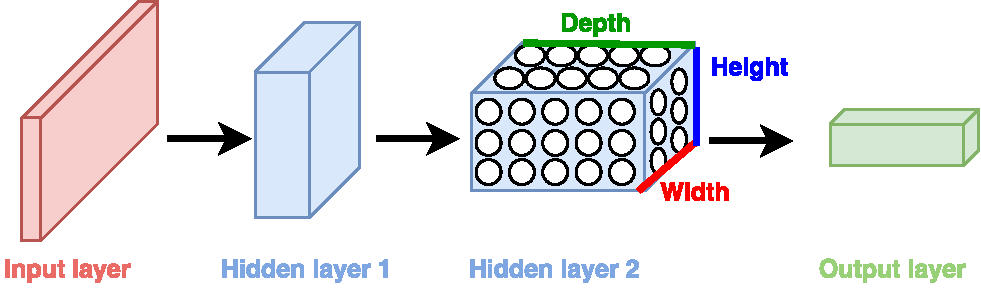
\includegraphics[width=1\textwidth]{Figures/NN_vs_CNN.pdf}
	\caption{A Convolutional Neural Network arranges its neurons in three dimensions (width, height, depth), as visualized in one of the layers. Every layer of a CNN transforms the 3D input volume to a 3D output volume of neuron activations. In this example, the red input layer holds the image, so its width and height would be the dimensions of the image, and the depth would be 3 (Red, Green, Blue channels) \cite{CNN_course}}.
	\label{fig:NN_vs_CNN}
\end{figure}

\subsubsection{Layers}
As described earlier a CNN is a combination of layers and every layer transforms one volume of activations into another through a differentiable function. CNN uses three main types of layers to build the architecture: Convolutional Layer, Pooling Layer, and Fully-Connected Layer (exactly as seen in regular Neural Networks on \Cref{fig:feedforward}). We will stack these layers to form a full CNN architecture. In reinforcement learning the pooling layer is not used, because they buy translation invariance - the network becomes insensitive to the location of an object in the image.

\subsubsection{Convolutional Layer}
The Convolutional layer is the main building block of a convolutional neural network. It does most of the computational heavy lifting. The convolutional layer consists of learnable filters. Every filter is spatially small (along width and height), but extends in the full depth of the input volume. An example of the first layer in a CNN is a filter with the size 5x5x3. During the first forward pass, the data is slid / convolved through each filter across the height and width of the input volume, and the dot products between the entries of the filter and the input at any position are computed. As the filter slides over the input volume it produces a 2-dimensional activation map. The activation map shows the responses of that filter at all spatial positions. The network will learn filters that activate when they see some type of visual feature - such as an edge of some orientation or a patch of some colors. On higher layers the network will learn to see more complex patterns: it could be honeycomb or wheel-like patterns. On each convolutional layer, there will be an entire set of filters, each layer will produce a separate 2-dimensional activation map. The activation maps will be stacked along the depth dimension and produce the output volume. 

When dealing with high dimensional inputs like images, it is impractical to connect neurons to all the neurons in the previous volume. It is smart to connect each neuron to only a local region of the input volume instead. The spatial extent of this connectivity is a hyperparameter called the receptive field of the neuron - equivalently this is the filter size. An illustration of the receptive field can be seen on \Cref{fig:Respective_field}

\begin{figure}[H]
	\centering
	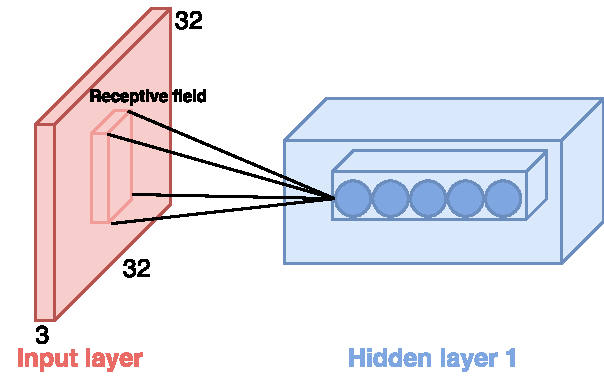
\includegraphics[width=0.7\textwidth]{Figures/Respective_field.pdf}
	\caption{An example input volume in red (e.g. a 32x32x3 CIFAR-10 image), and an example volume of neurons in the first Convolutional layer in blue. Each neuron in the convolutional layer is connected only to a local region in the input volume spatially, but to the full depth (i.e. all color channels). Note, there are multiple neurons (5 in this example) along the depth, all looking at the same region in the input \cite{CNN_course}}
	\label{fig:Respective_field}
\end{figure}

\textbf{Spatial arrangement}

The connectivity of each neuron in the convolutional layer to the input volume is described by the spatial arrangement. Spatial arrangement describes how many neurons there are in the output volume and how they are arranged. Three hyperparameters control the size of the output volume - depth, stride and zero-padding.

The first hyperparameter is the depth. It corresponds to how many filters the convolutional layer uses. Each filter looks for something different in the input. For example, the convolutional layer takes a raw image as an input, then the different neurons along the depth dimension may activate in the presence of various oriented edges or blobs of colors. A set of neurons that look at the same region of the input is called \textit{depth column} or \textit{fibre}.

Another hyperparameter is the stride. It defines how the filters slide over the input. If the stride is 1, then the filters move one pixel at a time. When the stride is 2, then the filters move 2 pixels at a time. This will produce spatially smaller output volumes.

The last hyperparameter to control the size of the output volume is the size of zero-padding. Zero-padding pads the input volume with zeros around the border. The good feature of zero-padding is that it controls the spatial size of the output volumes. This is useful to preserve the spatial size of the input volume, so that the input and output width and height are the same. 

The way to compute the spatial size of the output volume is by using a function of the input volume size ($\textbf{W}$), the receptive field size of the convolutional layer neurons ($\textbf{F}$), the stride with which they are applied ($\textbf{S}$), and the amount of zero padding used ($\textbf{P}$) on the border. The formula for calculating how many neurons "fit" is the following:
\begin{equation}
\frac{W-F+2P}{S}+1
\end{equation}    
An example for a 5x5 input and a 3x3 filter with stride 1 and zero-padding 1 the output would be of the spatial size 5x5:
\begin{equation}
\frac{5-3+2\cdot1 }{1}+1         \rightarrow             \frac{4}{1}+1 =5
\end{equation} 
And with stride 2 the output would be 3x3:
\begin{equation}
\frac{7-3+2\cdot1 }{2}+1         \rightarrow             \frac{4}{2}+1 =3
\end{equation} 
The visualization is provided on the figure below \Cref{fig:Spatial_size}: 

\begin{figure}[H]
	\centering
	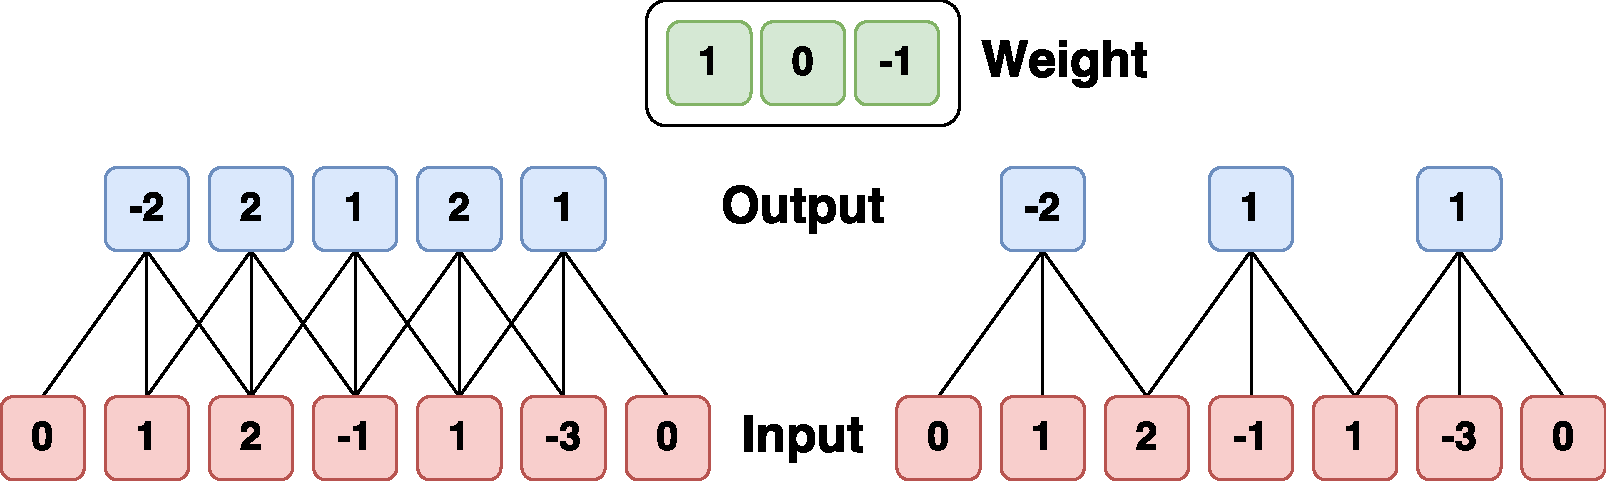
\includegraphics[width=1\textwidth]{Figures/Spatial_size.pdf}
	\caption{Illustration of spatial arrangement. The example is described above. In this example, there is only one spatial dimension (x-axis), one neuron with a receptive field size of F = 3, the input size is W = 5, and there is zero-padding of P = 1. \textbf{Left:} The neuron strided across the input in stride of S = 1. \textbf{Right:} The neuron uses stride of S = 2.
	The neuron weights are in this example [1,0,-1] (shown on very right), and its bias is zero. These weights are shared across all yellow neurons \cite{CNN_course}.
	}
	\label{fig:Spatial_size}
\end{figure} 

\subsubsection{Summary of convolutional layers}
The convolutional layer:
\begin{itemize}
	\item Accepts an input volume of size $W_1 \times  H_1 \times  D_1$
	\item Requires four hyperparameters:
	\begin{itemize}
		\item Number of filters $K$
		\item The receptive field size of the Convolutional Layer $F$ 
		\item The stride $S$
		\item The amount of zero-padding $P$ 
	\end{itemize}
	\item Outputs a volume of size $W_2 \times  H_2 \times  D_2$
	\begin{itemize}
		\item $W_2 = \frac{W_1-F+2P}{S}+1$
		\item $H_2 = \frac{H_1-F+2P}{S}+1$
		\item $D_2 = K$
	\end{itemize}
	\item In the output volume the $d$-th depth slide (of size $W_2 \times  H_2$) is the result of performing a valid convolution of the $d$-th filter over the input volume with a stride of $S$, and then offset by $d$-th bias
\end{itemize}

\subsubsection{Fully connected Layer}
The fully connected layer in CNNs is a traditional Multi-Layer Perceptron. The term “Fully Connected” implies that every neuron in the previous layer is connected to every neuron on the next layer as seen on \Cref{fig:feedforward}. The output from the convolutional layers represents a high-level feature of the input image. The purpose of the Fully Connected layer is to use these features for classifying the input images into various classes. 

Apart from classification the fully connected layer is also a cheap way to learn non-linear features. By combining these features, the classification of the network would be even better \cite{Fully_Connected_Layer}.

\subsection{Recurrent Neural Networks (RNNs)} \label{RNN}
Recurrent neural networks (RNN) are used when the patterns in data change with time. RNNs have a simple structure with a built-in feedback loop allowing it to act as a forecasting engine. RNNs are applied in a large range of applications, from speech recognition to driver-less cars. 

In feedforward neural networks the data flows in one direction only, whereas in RNN the output of the layer is added to the input of the same layer, and this layer represents the whole network. This results in a loop like network. The flow can be viewed or interpreted as a time passage where at each time-step the same layer receives it's own output from the previous time-step and adds it up to the input part together with the new data received \cite{RNNvideo}. 

Unlike feedforward ANNs, RNNs can work with sequences of data inputs and, subsequently, to output sequences of data in return. Not only RNNs use sequence of data, but also these sequences can vary in their size, so different sizes of sequences can be adapted by the RNN dynamically. Another key feature of the RNN is the dependency of the training examples. Unlike feedforward ANNs, where the training examples are independent of each other, the RNNs treat temporal dependencies, meaning that a sequence of e.g. words is usually dependent on what came before \cite{NeonRNN}. These new features open a new range of applications like image captioning (single input, sequence output), document classification (sequence input, single output), video frames classification (sequence input, sequence output), demand and supply chain planning forecasting (with added time delay) \cite{RNNvideo}.

In order to understand better the recurrent neuron functionality, the Figure \ref{Units} presents a comparison between the RNN unit and the linear unit used in feedforward ANNs.

\begin{figure}[H]
	\centering
	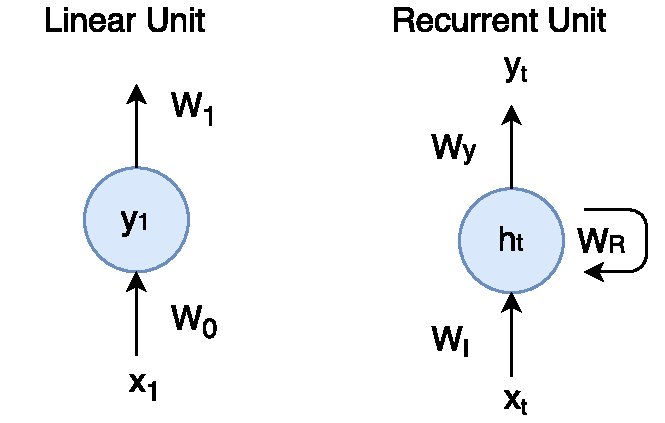
\includegraphics[width=0.5\textwidth]{Figures/RecurrentUnit}
	\caption{Linear vs. Recurrent unit}
	\label{Units}
\end{figure}
A linear unit's output is the input $x_{j}$ times the weight matrix $W_{ij}$ which is then passed to an activation function $g$.
\begin{equation}\label{linearOutput}
y_{i}=g(\sum_{j}W_{ij}x_{j}+b)
\end{equation}

The recurrent unit is composed of a linear unit, but then it adds a recurrent weight $W_{R}$, therefore the output $h^{(t)}$ depends on both the input $x_{t}$ and the activity at the previous time-step. To retrieve an output $y_{t}$ from the layer, a non linear activation function $g_{y}$ is applied to the $h^{(t)}$ \cite{NeonRNN}.
\begin{equation}\label{recurrentOutput}
\begin{aligned}
h^{(t)}&=g_{h}(W_{I}x^{(t)}+W_{R}h^{(t-1)}+b_{h})\\
y^{(t)}&=g_{y}(W_{y}h^{(t)}+b_{y})
\end{aligned}
\end{equation}

For example, in case of word prediction, the input of a unit can be a word, and the output of that unit would be the predicted next word that follows the one that was input; then, when the next input comes in at the next time-step, the process is applied, but also with the activity at the previous time-step taken into account.

The training of RNNs is different than that of the other ANNs, because RNNs emit an output at each time-step, and, therefore, there is a cost function at each time-step, whereas before, in feedforward networks, it was necessary to run the input through the whole network in order to get an output comparable to the one and only cost function. Another special characteristic of the RNNs is that the weights $W_{R}$ are shared across the network. So, the gradients from all the time-steps can be combined together to obtain the weights update and do back-propagation. But, because of the shared weights the update would scale with the size of the $W_{R}$, the back-propagation has to be done all the way until time-step zero, which causes the problem of vanishing and exploding gradients \cite{NeonRNN}.

\subsubsection{Gating in RNN}
In order to address the problems of training deep RNNs there are different solutions available. Among the known solutions are the use of the \textit{Root Mean Square Propagation} (RMSProp) optimizer for learning rate adjustment, clipping gradients, ReLu activation functions, special weight initialization, or to use \textit{gating} \cite{NeonRNN}. Gating is a technique for deciding when to forget the current input, and when to remember it for future time steps \cite{RNNvideo}. The most famous approaches are \textit{long short-term memory} (LSTM) and \textit{gated recurrent units} (GRU).

LSTM has at it's core a memory cell $C$ with a recurrent weight $W_{C}=1$ that inherits the activity of the previous time-step. This memory cell has three manipulations: \textit{forget} (flush the memory), \textit{input} (add to the memory), and \textit{output} (retrieve from the memory) \cite{NeonRNN}. The activity of the memory cell $C_{t}$ is taken and passed through a tanh activation function and multiplied by the \textit{gate}. The gate is an affine layer, or a 'standard' feedforward ANN layer, that has as inputs $x_{t}$ at the current time-step and $h_{t-1}$ of the previous time-step that are together multiplied by the weight $W_{0}$, summed and passed through the sigmoid activation function $\sigma$ to return a vector of numbers between $0$ and $1$. The gate operation for generating the \textit{output} $h_{t}$, or for getting the information from the memory cell $C_{t}$, is presented in the following equation:
\begin{equation}\label{gate}
\begin{split}
h_{t}&=\sigma(W_{0}\cdot \left [ x_{t} h_{t-1} \right ]+b_{0})\odot \textup{tanh}(C_{t})\\
&=o_{t}\odot \textup{tanh}(C_{t})
\end{split}
\end{equation}

The same approach is used for the \textit{forget} operation $f_{t}$. A layer before the final output is introduced, but with different weights, $W_{f}$. If the output of the forget gate is $0$, means that the memory has been flushed completely, whereas if the output is all $1$s then the memory retained everything \cite{NeonRNN}. 

The \textit{input} for the next time-step has two affine layers, one for generating new input $\widetilde{C_{t}}$ for the memory cell with the weights $W_{C}$ and tanh activation function, and another one $i_{t}$ that modulates the input and writes it into the memory cell with the weights $W_{i}$ and the sigmoid activation function $\sigma$. 

All the components of the LSTM structure are vectors with numbers between $0$ and $1$, and they can be handled to perform either of the available manipulations. The summarized presentation of the LSTM components with the corresponding affine layers is illustrated in the Figure \ref{LSTMcore} \cite{NeonRNN}.
\begin{figure}[H]
	\centering
	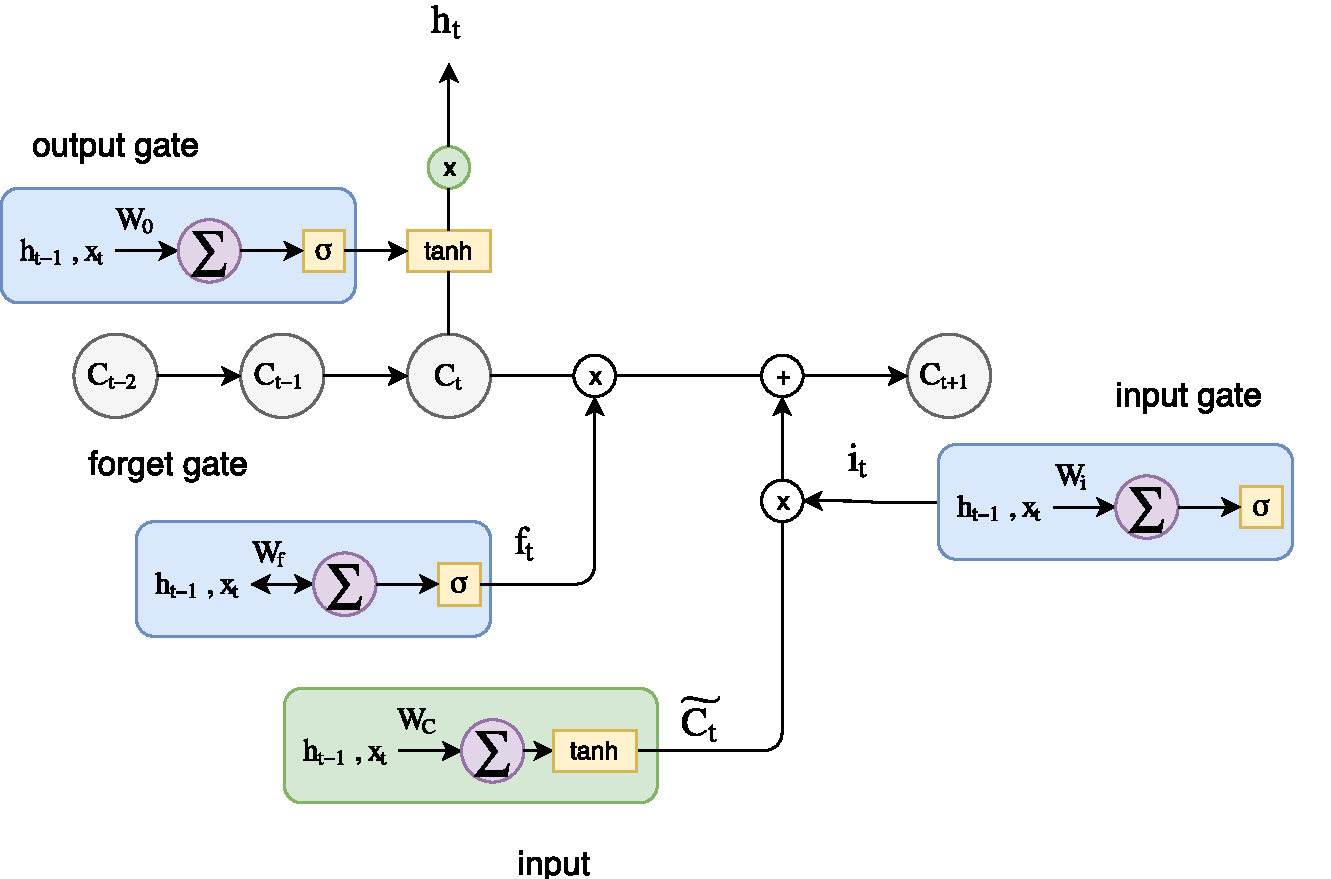
\includegraphics[width=0.9\textwidth]{Figures/LSTM}
	\caption{LSTM functionality}
	\label{LSTMcore}
\end{figure}

Having explained the LSTM functionality, the formula for computing the next time-step activity $C_{t+1}$ is the following:
\begin{equation}\label{LSTM}
C_{t+1}=f_{t}\odot C_{t}+i_{t}\odot \widetilde{C_{t}}
\end{equation}

The GRU gating approach is a simplified version of the LSTM. It actually combines all the gates into a single update:
\begin{equation}\label{GRU}
\begin{aligned}
h_{t}&=(1-z_{t})\cdot h_{t-1}+z_{t}\cdot \widetilde{h_{t}}\\
z_{t}&=\sigma(W_{z}\cdot[h_{t-1},x_{t}]) \textup{ (update gate)}\\
\widetilde{h_{t}}&=\textup{tanh}(W\cdot[r_{t}\cdot h_{t-1},x_{t}]) \textup{ (input gate)}\\
r_{t}&=\sigma(W_{r}\cdot[h_{t-1},x_{t}]) \textup{ (remember gate)}
\end{aligned}
\end{equation}
\section{Previous Research}
\label{Previous_Research}
This section summarizes four important papers, which all have made a big impact in the area of deep reinforcement learning. Each paper is described with the important concepts in the represented paper. It will give a overview of state of the art in the area of deep reinforcement learning.   

\subsection{Playing Atari with Deep Reinforcement Learning }\cite{DBLP:journals/corr/MnihKSGAWR13}
This paper was published in 2013 by DeepMind Technologies. It is the first paper to make a deep learning model to successfully learn control policies directly from sensory input using reinforcement learning. 

The paper present some of the challenges by using deep learning to do reinforcement learning. One of the challenges is deep learning algorithm requires large amount of handlabelled training data. Another challenge is the delay between action and resulting reward, which can be thousands timesteps long.The paper demonstrates that a convolutional neural network can overcome these challenges. 

The goal is to connect a reinforcement learning algorithm to a deep neural network which uses RGB images and process training data by using stochastic gradient update. The starting point for this approach is to use Tesauro's TD-Gammon \cite{Tesauro:1995:TDL:203330.203343} architecture. The network is different from TD-Gammon and other online approaches, because it uses a technique known as experience replay, where the agent store the agents experiences at each time-step.

The input to the neural network is an $84 x 84 x 4$ image. The output from the neural network is a single output for each valid actions. The architecture of the network can be seen on \Cref{fig:playing_atari}   
\begin{figure}[H]
	\centering
	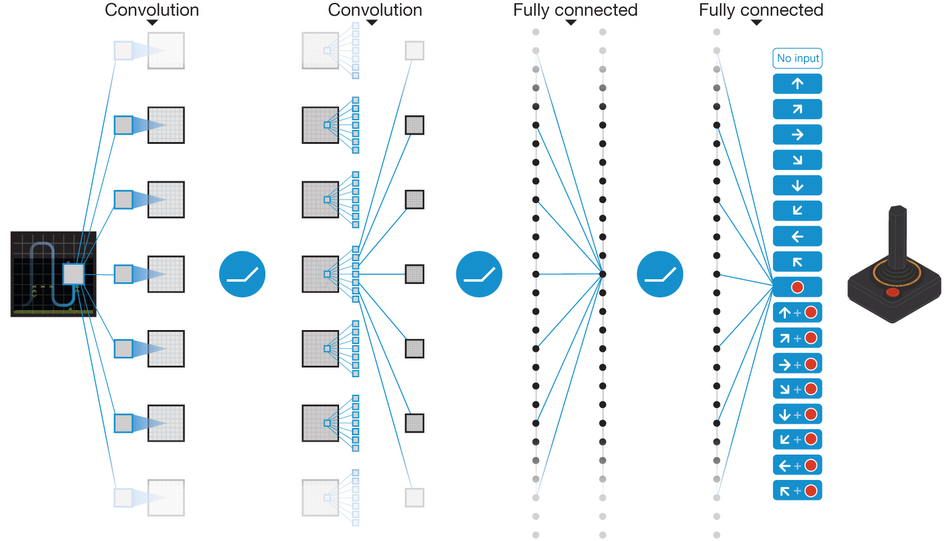
\includegraphics[width=0.7\textwidth]{Figures/TheoreticalBackground/playing_atari.jpg}
	\caption{The arhitecture of the network used in the article "Playing Atari with Deep Reinforcement Learning"}
	\label{fig:playing_atari}
\end{figure} 

This network is tested on seven Atari games, and the approach in this paper gave state-of-the-art result in six of the seven games. Finally it showed better performance than a expert human player in three out of the seven games.  

\subsection{Mastering the Game of Go with Deep Neural Networks and Tree Search}\cite{Silver_2016}
This paper introduce a new approach to compete in the classic game Go, the paper was published in 2016. The game of Go is the most challenging classic game for artificial intelligence, due to the enormous search space and the difficulty of evaluating board positions and moves. 

They employ a similar architecture as in \cite{DBLP:journals/corr/MnihKSGAWR13}. Here they pass in the board position as a $19 x 19$ image and use convolutional layers to construct a representation of the position. It uses neural networks to reduce the search space, this is done by use of value networks to evaluate board position and policy networks to select moves.

The way they trained the Neural Network started with training a supervised learning policy network, directly from expert human moves. Next training the reinforcement learning policy network is done by improving the supervised learning network by optimizing the final outcome of games og self-play. The final atep of training, is to train the value network, that predict the winner of the games played by the reinforcement learning policy network against it self.   

By combining tree search with policy and value networks, \textit{AlphaGo} has reached a professional level in Go. In March 2016 \textit{AlphaGo} won 4-1 against the legendary Lee Sedol , the top Go player in the world over the past decade.  

\subsection{Asynchronous Methods for Deep Reinforcement Learning}\cite{DBLP:journals/corr/MnihBMGLHSK16}
This is another paper from the team behind \cite{DBLP:journals/corr/MnihKSGAWR13}, and was published in 2016. This paper provide a very different paradigm for deep reinforcement learning. Instead of experience replay, it asynchronously execute multiple agents in parallel, on multiple instances of the environment. 

This simple idea enables much larger spectrum of on-policy reinforcement learning algorithm as well as off-policy reinforcement learning algorithm, to be applied robustly and effectively using deep neural networks.  It also offers practical benefits, this experiment is able to run on a single machine with a standard multi-core CPU, instead of specialized such as GPUs.

The paper presents asynchronous versions of four standard reinforcement algorithms used on different platforms. The platform used is a simulator for Atari 2600, Torcs 3D car racing simulator, Mujoco and Labyrinth. The asynchronous advantage actor-critic (A3C) algorithm was the best performing agent on all the platforms.

The asynchronous advantage actor-critic (A3C) beats state of the art result in 26 of 57 Atari games. This is a big improvement from previously reinforcement networks. When trained on the Atari domain using 16 CPU cores, the proposed asynchronous algorithm train faster than Deep Q-Network trained on an Nvidia K40 GPU, with A3C surpassing the state of the art in half the training time.   

\subsection{Deep Reinforcement Learning framework for Autonomous Driving} \cite{Sallab:2017:2470-1173:70}
This paper is motivated by the papers \cite{DBLP:journals/corr/MnihKSGAWR13} and \cite{Silver_2016}. It propose a framework for autonomous driving using deep reinforcement learning, the paper was published in 2017. It is relevant because it is difficult to handle autonomous driving as a supervised learning problem due to interactions with the environment. It also integrates recent work on attention models, to focus on relevant information, thereby reducing the computational complexity.

They propose a framework for an end-end autonomous driving model that takes in raw sensor input and output the driving actions. The model is able to handle partially observable scenarios. 

The framework can be seen on \Cref{fig:Framework_article} 

\begin{figure}[H]
	\centering
	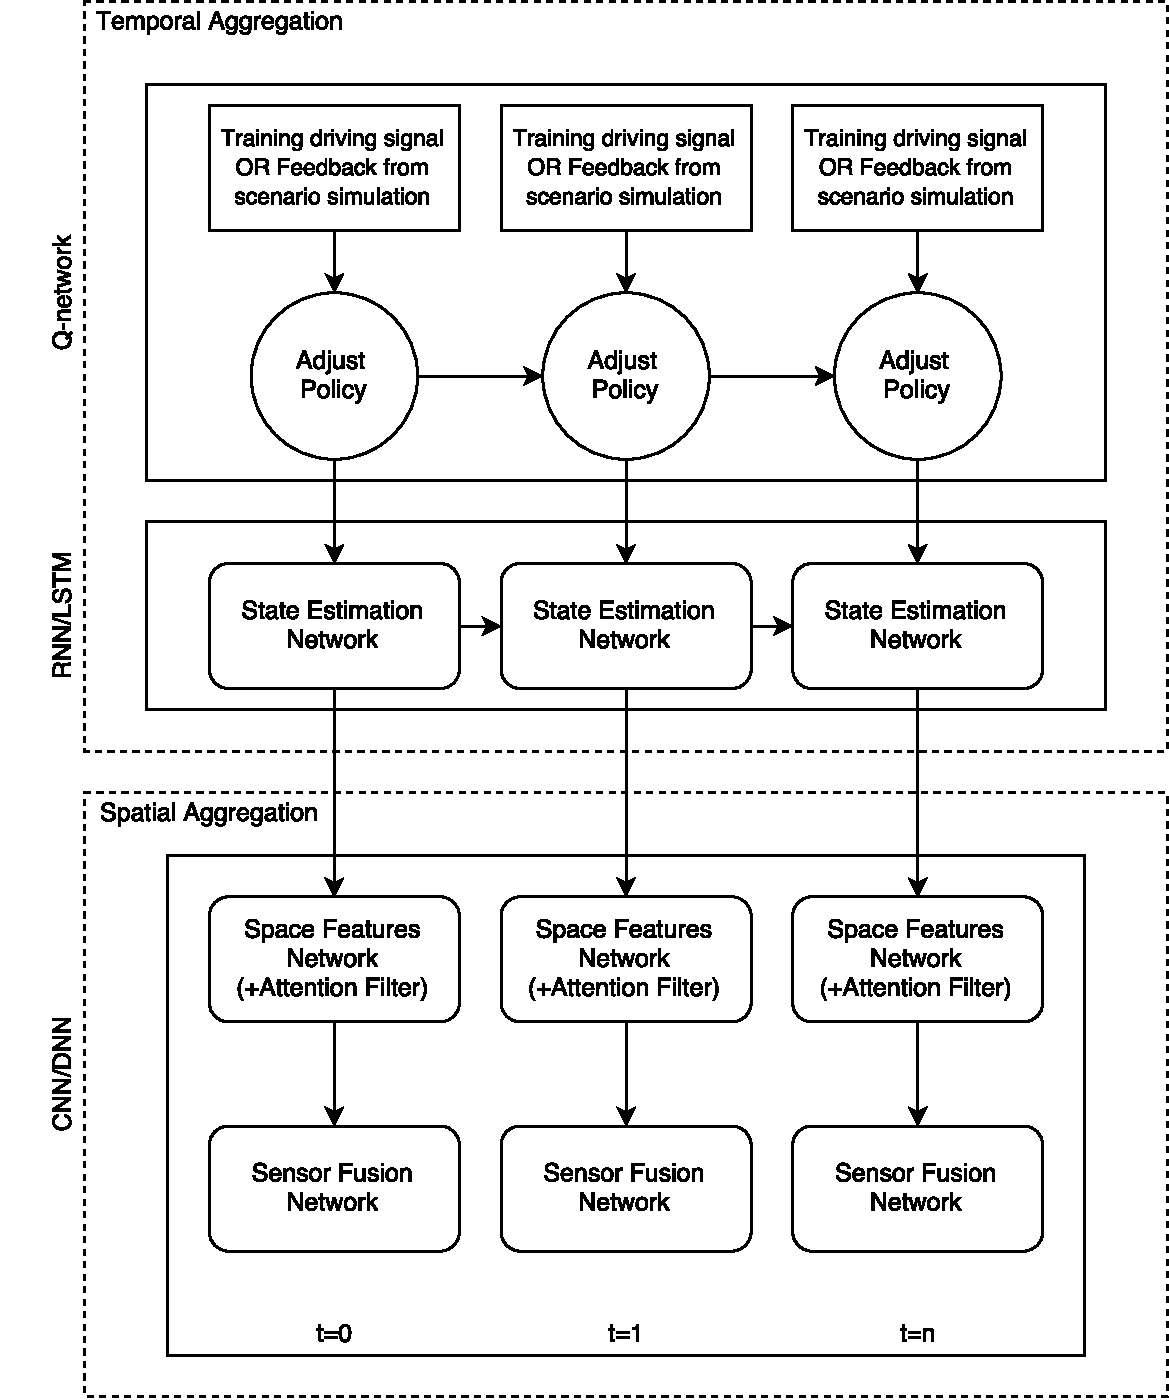
\includegraphics[width=0.8\textwidth]{Figures/TheoreticalBackground/Framework_article}
	\caption{Framework from the article "Deep Reinforcement Learning framework for Autonomous Driving}
	\label{fig:Framework_article}
\end{figure}
 
\chapter{Methods}
\label{chap:projectdef}
This chapter will explain the methods implemented in this project. The methods used is state of the art methods in deep reinforcement learning, they are decided from their impact in the area. One of the companies which is in front of developing new reinforcement learning methods is DeepMind. All the methods in this project is method published by DeepMind in the recent years. A figure to show an overview of the methods used in this project, can be seen on \Cref{fig:Methods_deepmind}     

\begin{figure}[H]
	\centering
	
\includegraphics[width=1.25\textwidth]{Figures/Architecture/Methods_deepmind.pdf}
	\caption{Timeline of methods published by DeepMind. Methods explain and implemented in this chapter is in a red box.   }
	\label{fig:Methods_deepmind}
\end{figure}

All the methods shown on \Cref{fig:Methods_deepmind} is method found on DeepMind's website \cite{Publications_Deepmind}. The first method used and explained is the DQN (Deep Q-Network) from the paper \cite{DBLP:journals/corr/MnihKSGAWR13}. A short description of this method is also found in \Cref{Previous_Research}, and had a big impact on deep reinforcement learning.    

The next method this project has worked with is the DDPG (Deep Deterministic Policy Gradient) this method is the first method used for continuous control. The method is from the paper \cite{DBLP:journals/corr/LillicrapHPHETS15}. 

By looking at the timeline the next two algorithm by DeepMind is not implemented and explained. The DDQN (Double Deep Q-Network) is a more advance version of the DQN and can be found in the paper \cite{DBLP:journals/corr/HasseltGS15}. The other method is the one DeepMind used to beat Lee Sedol in the game Go, a short description of the paper can be found in \Cref{Previous_Research}. An explanation of the Method DeepMind used in the game of Go, can be found in the paper \cite{Silver_2016}. 

The last method explained and implemented in this project is the A3C (Asynchronous Advantage Actor Critic) method, this is a method which uses different agent to train in the environment. A3C is the method which has been used mostly in this project, because it is the method which performed best. The method was published by DeepMind in the paper \cite{DBLP:journals/corr/MnihBMGLHSK16}.  

All the method is implemented and tested in this project to explore the differences and get a knowledge of how they worked. The DDPG and A3C is implemented in the TORCS environment, which is also explained in this chapter. 




%\begin{figure}[H]
%	\centering
% 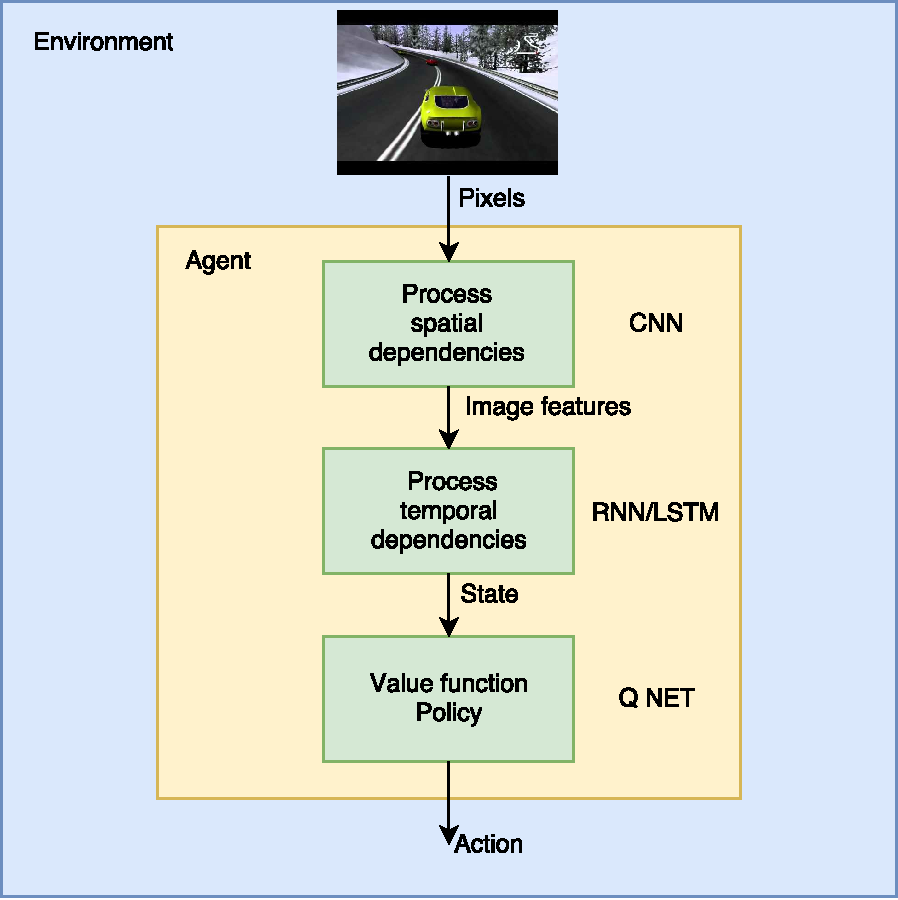
\includegraphics[width=0.3\textwidth]{Figures/ProjectFramework/Project_framework_diagram}
%	\caption{The framework for the system used in this project}
%	\label{fig:Project_framework}
%\end{figure}

\section{Deep Q Networks}
\label{sec:DQN}
The first deep reinforcement learning network there has been created in this project is the Deep Q Network. The Deep Q Network was first time described in the paper "playing Atari with Deep reinforcement learning" \cite{DBLP:journals/corr/MnihKSGAWR13} published by DeepMind. In this paper they learned the computer to play Atari 2600 video games. The computer only observed the screen pixels from the game, and received a reward when the game score increased. The result was remarkable, because the games and the goals in the games are very different. The same architecture was used for seven different games. In 3 of the seven games the computer performed better than the best human. 

To understand the problem the Deep Q Network solved, it is easier to use an example, here we use the game Breakout as an example. In this game you control a paddle at the bottom of the screen, and have to clear the bricks in the top of the screen. This is done by bouncing a ball between the paddle and the bricks. Each time a brick is hit it disappears and the game score increases. The game can be seen on figure \Cref{fig:Atari_breakout}

\begin{figure}[H]
	\centering
	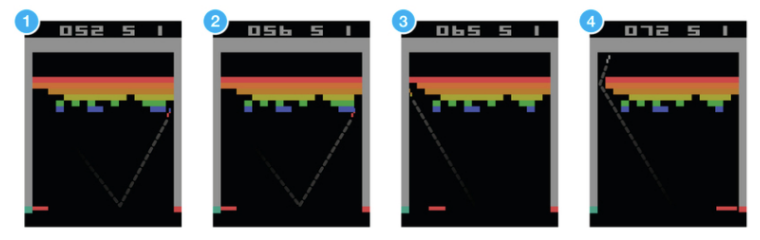
\includegraphics[width=1\textwidth]{Figures/Architecture/DQN/Atari_breakout.png}
	\caption{Atari Breakout game. Image credit: DeepMind\cite{DBLP:journals/corr/MnihKSGAWR13} }
	\label{fig:Atari_breakout}
\end{figure}

To teach a Network how to play this game, the input to the network is the screen images, and the output is the actions of the game: left, right or fire (to launch the ball). One approach to this problem is to treat it as a classification problem - for each screen decide if the paddle should move left, right or press fire. To do this lots of training examples is needed. The problem about this approach is thats really how human learns, we don't need someone to tell us million times which move to choose at each screen. Instead human just need occasional feedback that we did the right thing, and then learn from it ourself. This is the task reinforcement learning tries to solve, more of the reinforcement learning theory can be read in \textbf{Reference to Theory chapter}.

While the idea is quite intuitive, in practice there are numerous challenges. One of the challenges is when hitting a brick and the reward is received, it often has nothing to do with the actions (paddle movement) just before the reward was received. All the work was done when the paddle was positioned correctly and bounced the ball back. This is called the credit assignment problem – i.e., which of the preceding actions was responsible for getting the reward and to what extent.

Another challenge is when a strategy is found and a certain reward is received, should the program stick with that strategy or experiment with something that could lead to a bigger reward. This is called the explore-exploit dilemma – should you exploit the known working strategy or explore other, possibly better strategies. 

The screen pixels obtain most of the relevant information of the game situation, except speed and direction of the ball. This could be covered by having two consecutive screens. 

\subsection{Preprocessing}
The DeepMind paper use preprocessing where the take the last four screen images, resize them to 84x84 and convert to grayscale with 256 gray levels. This will give $256^{84x84x4} \approx 10^{67970}$ possible game states. This will give $10^{67970}$ rows in the imaginary Q-table - more than the number of atoms in the universe. Many pixel combinations never occur, so possible represent it as a sparse table containing only visited states. Most of the states are rarely visited and it would take a lifetime of the universe to the q-table to converge. It should also be possible to have a good guess for Q-values for states we have never seen. 

To do this deep learning comes in to the picture. Neural networks are extremely good at coming up with good features for highly structured data. A way neural networks can be used in reinforcement learning is it could represent the Q-function, where it takes the state (four game screens) and action as an input and output the corresponding Q-value. Another way is to only take game screens as input, and output the Q-value for each possible action. The second approach has the advantages, that if we want to perform a Q-value update or choose the action with the highest Q-value, it can be done by only doing one forward pass in the network and have all Q-values for all possible actions. The two different approaches to use neural network to represent the Q-function can be seen on \Cref{fig:DQN_two_approach}.              


\begin{figure}[H]
	\centering
	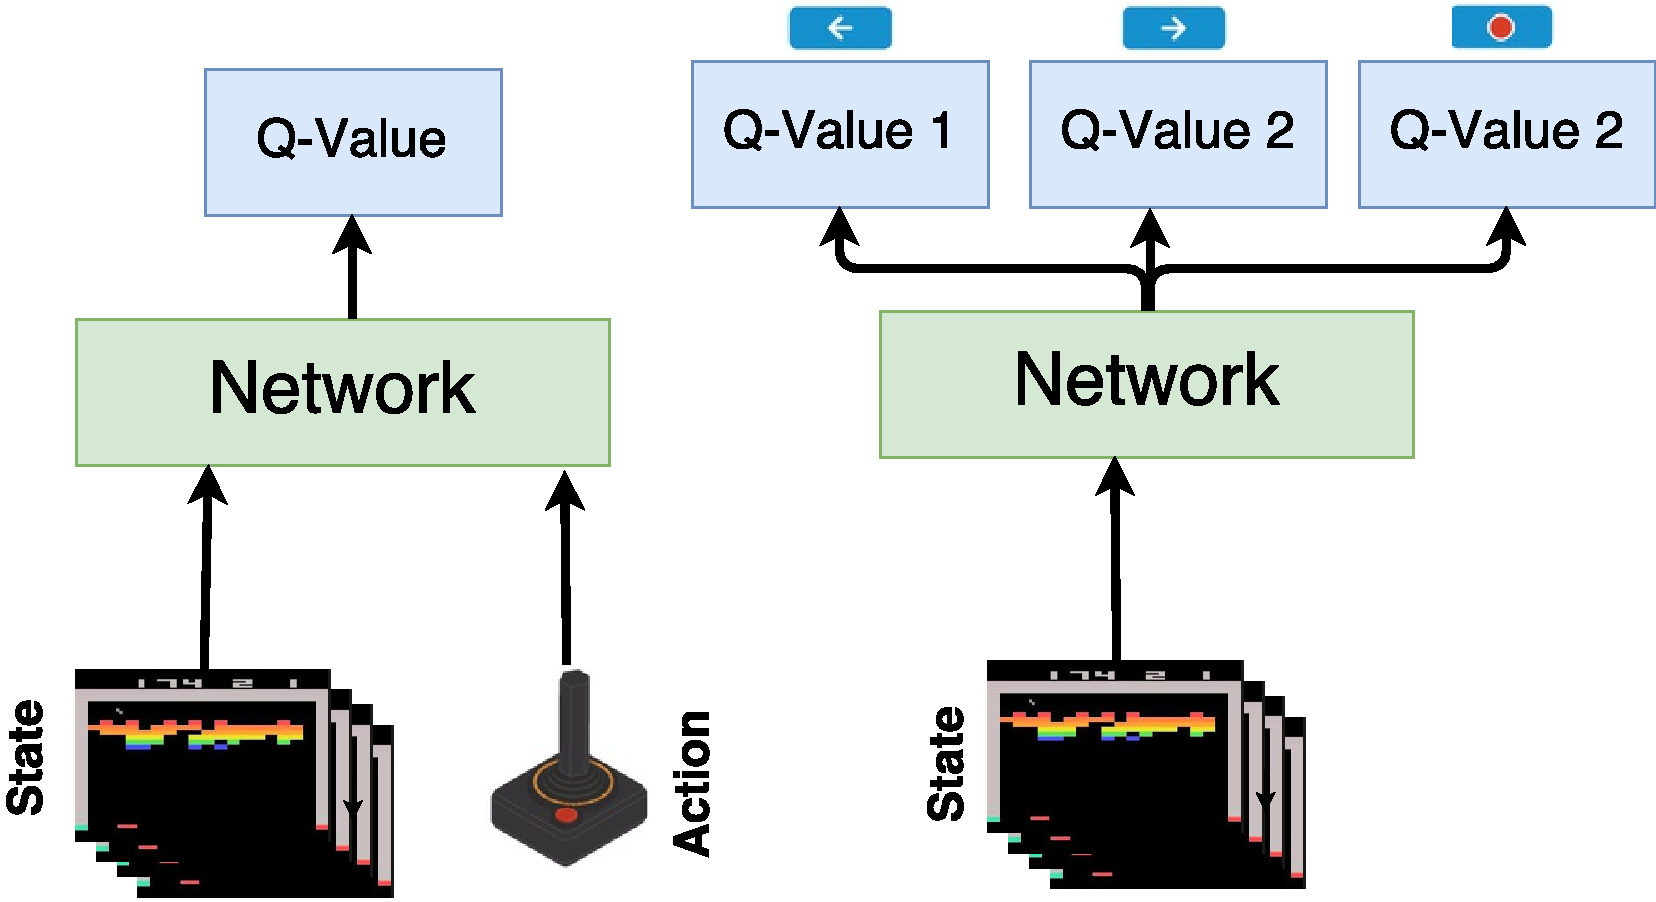
\includegraphics[width=1\textwidth]{Figures/Architecture/DQN/DQN_two_approach.pdf}
	\caption{Left: Naive formulation of deep Q-network. Right: More optimized architecture of deep Q-network, used in DeepMind paper.} 
	\label{fig:DQN_two_approach}
\end{figure}    

\subsection{Network}
The network architecture that DeepMind used can be seen on the table below \Cref{tab:DQN_network}. 

\begin{table}[H]
	\centering
	\caption{Architecture of the Deep Q Network used by DeepMind}
	\label{tab:DQN_network}
	\begin{tabular}{|l|c|c|c|c|c|c|}
		\hline
		\rowcolor[HTML]{9B9B9B} 
		\multicolumn{1}{|c|}{\cellcolor[HTML]{9B9B9B}\textbf{Layer}} & \textbf{Input} & \textbf{Filter size} & \textbf{Stride} & \textbf{Num filters} & \textbf{Activation} & \textbf{Output} \\ \hline
		\cellcolor[HTML]{FFFFFF}\textbf{conv1}                       & 84x84x4        & 8x8                  & 4               & 32                   & ReLU                & 20x20x32        \\ \hline
		\rowcolor[HTML]{C0C0C0} 
		\textbf{conv2}                                               & 20x20x32       & 4x4                  & 2               & 64                   & ReLU                & 9x9x64          \\ \hline
		\cellcolor[HTML]{FFFFFF}\textbf{conv3}                       & 9x9x64         & 3x3                  & 1               & 64                   & ReLU                & 7x7x64          \\ \hline
		\rowcolor[HTML]{C0C0C0} 
		\textbf{fc4}                                                 & 7x7x64         &                      &                 & 512                  & ReLU                & 512             \\ \hline
		\cellcolor[HTML]{FFFFFF}\textbf{fc5}                         & 512            &                      &                 & 18                   & Linear              & 18              \\ \hline
	\end{tabular}
\end{table}

The network can be seen as a classical convolutional neural network with three convolutional layers, followed by two fully connected layers. One of the things which makes this neural network different from the classical neural networks used for image recognition, is no poling layers are used. No pooling layers are used because they buy translation invariance -  the network becomes insensitive to the location of an object in the image. This is okay for image recognition, but for games where the location of the ball is important for deciding the potential reward.  

As seen on \Cref{fig:DQN_two_approach} the input to the network is four 84x84 grayscale game screens. The output of the network are a Q-value for each action, 18 actions for atari games (in breakout there are only 3 actions). The Q-value can be any real number, which make it a regression task. The optimization of the Q-values can be done by a squared error loss. 

\begin{equation}
L=\frac{1}{2}[r+max_{a'}Q(s',a')-Q(s,a)]^2
\end{equation}  

In the squared error loss function is $r+max_{a'}Q(s',a')$ the target, and $Q(s,a)$ is the prediction. Given a transaction <s,a,r,s'>, the Q-table is updated by the following steps:
\begin{enumerate}
	\item Do a feedforward pass for the current state s to get predicted Q-values for all actions.
	\item Do a feedforward pass for the next state s’ and calculate maximum overall network outputs $max_{a'}Q(s',a')$
	\item Set Q-value target for action to $r+max_{a'}Q(s',a')$ (use the max calculated in step 2).For all other actions, set the Q-value target to the same as originally returned from step 1, making the error 0 for those outputs. 
	\item Update the weights using backpropagation.
\end{enumerate}

\subsubsection{Experience Replay}
The approximation of the Q-values using non-linear functions is not very stable. There is many tricks to make i converge. And the problem with this method is it takes long time to converge almost a week on a single GPU. 

The most important tricks is experience replay. During gameplay all the experiences <s, a, r, s’> are stored in a replay memory. While training the network random minibatches are used instead of the recent transition. This breacks the similarity of training samples, and there by avoid the network to reach a local minimum. Experience replay makes the training task more similar to usual supervised learning, which simplifies debugging and testing the algorithm. A way this could be done is by collecting experience from human players, and train on those experiences.
  
\subsubsection{Exploration-Exploitation}
In reinforcement learning the Exploration-Exploitation dilemma, is if the agent should explore or exploit. First when the Q-table or Q-network is initialized randomly, then the prediction of the action is equally random, this is called exploration. As a Q-function converges, it returns more consistent Q-values and the amount of exploration decreases. Q-learning use the exploration as part of the algorithm. But this exploration is “greedy”, it settles with the first effective strategy it finds.

A simple way to do this is to use the $\epsilon$-greedy exploration - with probability $\epsilon$ choose a random action, otherwise go with the “greedy” action with the highest Q-value. DeepMind decreases $\epsilon$ over time from 1 to 0.1. This means in the beginning the system makes random actions to explore the state space maximally, and in the end it settles to a fixed exploration rate.  
        
\section{Deep Deterministic Policy Gradient (DDPG)}
As mentioned in \Cref{sec:DQN} the Deep Q Network solves problems with high-dimensional observation space. But the problem is it can only handle discrete and low-dimensional action space. Many task of interest, most notably physical control tasks, have continuous (real valued) and high dimensional action spaces. The problem with the Deep Q Network is it cannot be applied to continuous domains since it relies on finding the action that maximizes action-value function. In the continuous valued case requires an iterative optimization process at every step. \cite{DBLP:journals/corr/LillicrapHPHETS15}

An obvious approach to adapting the Deep Q Network method to continuous domain is to simply discretize the action space. This have many limitation, most important the curse of dimensionality - the number of actions increases exponentially with the number of degrees of freedom. An example is the human arm is a 7 degrees of freedom system, with a assumption discretization $a_i \sim  \{-k,0,k\}$ for each joint leads to an action space with dimensionality: $3^7 = 2187$. This problem just become bigger with a finer discretion. Such a large action space makes it difficult to explore efficiently. Discretization of action spaces throws away information of the action domain.

The Deep Deterministic Policy Gradient try to solve these problems. The Deep Deterministic Policy Gradient method is a model-free off-policy actor-critic algorithm using deep function approximators that can learn policies in high-dimensional, continuous action space. 

The DDPG algorithm uses some of the some of the deep learning tricks, which was used in the Deep Q Network (DQN) see \Cref{sec:DQN}. To explain more about this algorithm a car simulation environment called "Torcs" is used see \textbf{REF TO TORCS SECTION}. \cite{DDPG_Torcs} 

\subsection{Algorithm}
Even with the DDPG using some of the tricks from the DQN algorithm, it is not straight forward to apply the Q-learning to continuous action space. It is because in continuous action spaces finding a greedy policy requires an optimization of \textit{$a_t$} at every time step - this optimization is too slow to be practical with large, unconstrained function approximators and non trivial action spaces. Here is instead used an actor-critic approach based on the DPG (deterministic policy gradient) algorithm \cite{DBLP:conf/icml/SilverLHDWR14}

The DPG algorithm use a parameterized actor function $\mu(s|\theta^\mu)$ which specifies the current policy by deterministically mapping states to a specific action. The critic $Q(s,a)$ is learned by using the Bellman equation as in Q-learning. The actor is updated by applying the chain rule to the expected return from the start distribution J with respect to the actor parameters:
\begin{equation}
\triangledown_{\theta^\mu} J \approx \mathbb{E}_{s_t \sim \rho^\beta} [\triangledown_{\theta^\mu}Q(s,a|\theta^Q)|_{s=s_t , a=\mu(s_t|\theta^\mu)}]  
\newline
\end{equation}
\begin{equation}
\triangledown_{\theta^\mu} J = \mathbb{E}_{s_t \sim \rho^\beta} [\triangledown_{a}Q(s,a|\theta^Q)|_{s=s_t , a=\mu(s_t)} \triangledown_{\theta_\mu}\mu(s|\theta^\mu)|_{s=s_t} ]
\end{equation} 

This was proved that it is the policy gradient - the gradient of the policy performance. 

Introducing non-linear function approximators means that convergence is no longer guaranteed. The approximators is essential to learn and generalize on large state spaces. The DDPG contribution is to provide modification to DPG inspired of the succes of the DQN, which allow it to use neural networks function approximators to learn in state and action space online. 

One of the challenges of using neural networks for reinforcement learning is that most optimization algorithms assume that the samples are independently  and identically distributed. To solve this problem a replay buffer is used, it is sampling a minibatch uniformly from the buffer - more about the replay buffer see \Cref{sec:DQN}. Because the DDPG is a off-policy algorithm, the replay buffer can be large, allowing the algorithm to benefit from learning across a set of uncorrelated transition.
              
\section{TORCS (The Open Racing Car Simulator)}
\label{sec:TORCS}
The environment to use in reinforcement learning is important, because it is here all the learning will be done. This project is using reinforcement learning in autonomous driving. After reading the post \cite{DDPG_Torcs} that uses TORCS in combination with Gym-TORCS. It was decided that this project will use the same environment, because it seems like it will make a good simulation environment for the task in the project. It is also an environment DeepMind has used to test their algorithms \cite{DBLP:journals/corr/LillicrapHPHETS15} and \cite{DBLP:journals/corr/MnihBMGLHSK16}, it is thereby a well-known environment to use in reinforcement learning. 

The Open Racing Car Simulator or TORCS is a highly portable multi-platform car racing simulation. It is used as ordinary car racing game, as AI racing game and as a research platform. The source code of TORCS is licensed under the GPL ("Open Source") \cite{TORCS_website}. 

Gym-TORCS is a reinforcement learning environment in the TORCS domain. It is made to have an interface which matched Open-AI - A toolkit for developing and comparing reinforcement learning algorithms. It supports teaching agents everything from walking to playing games like Pong or Go \cite{OPENAI_website}. It is smart to match the Open-AI interface because it combines a lot of environment to solve different reinforcement learning tasks. This is done by a simple interface to make it easier to use. \cite{Gym_TORCS_website}. 

Some points why TORCS is useful as an environment for reinforcement learning:
\begin{itemize}
	\item The AI can learn how to drive
	\item It is possible to visualize how the neural networks learn over time and inspect its learning process. Instead of only looking at the final result.
	\item It is easy to visualize when the neural network gets stuck in a local minimum.
	\item Gives an understanding of machine learning technique in automated driving, which is important for autonomous driving technologies 
\end{itemize}

Some pictures from TORCS can be found on \Cref{fig:torcs_screenshots} the below:
\begin{figure} [H]
	\centering
	\begin{subfigure}{.20\textwidth}
		\centering
		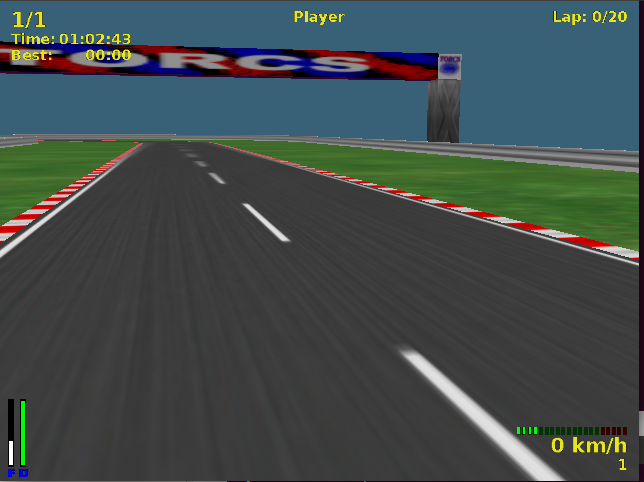
\includegraphics[width=25mm, height=25mm]{Figures/Architecture/Torcs/torcs_2.png}
	\end{subfigure}
	\begin{subfigure}{.20\textwidth}
	\centering
	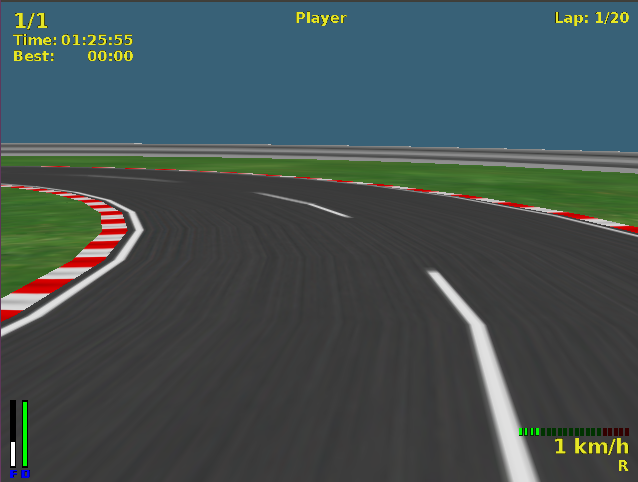
\includegraphics[width=25mm, height=25mm]{Figures/Architecture/Torcs/torcs_3.png}
    \end{subfigure}
	\begin{subfigure}{.20\textwidth}
	\centering
	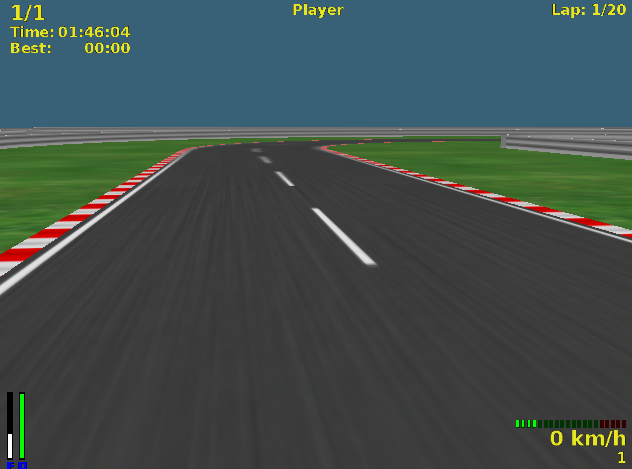
\includegraphics[width=25mm, height=25mm]{Figures/Architecture/Torcs/torcs_4.png}
	\end{subfigure}
	\begin{subfigure}{.20\textwidth}
	\centering
	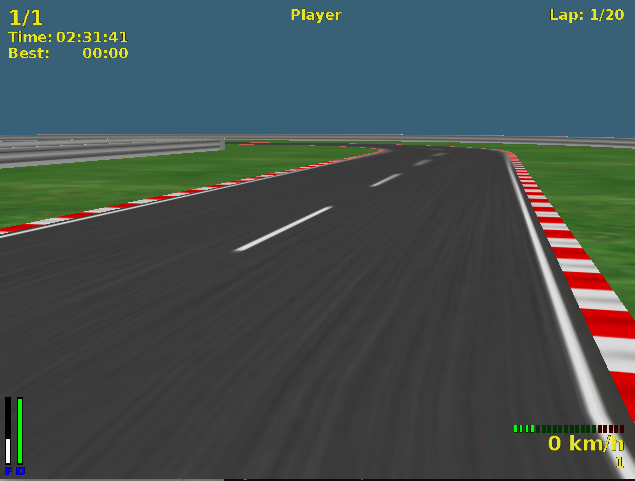
\includegraphics[width=25mm, height=25mm]{Figures/Architecture/Torcs/torcs_5.png}
	\end{subfigure}
	\caption{Screenshots from the TORCS environment}
	\label{fig:torcs_screenshots}
\end{figure}
      
\subsection{Uses in this project}      
The way this environment has been used, is by getting information from the TORCS domain. This information could be the game screen, so the pixels of the game. Another thing the environment has been used for, is to send commands to the game - like steering the car. 

The reinforcement learning should be able to train a network, where the input to the network is the information coming from the game. The output from the network is the determined action, which then will be send to the game. This interaction between the game and the network can be seen on \Cref{fig:TORCS_interaction}.    
 
\begin{figure}[H]
	\centering
	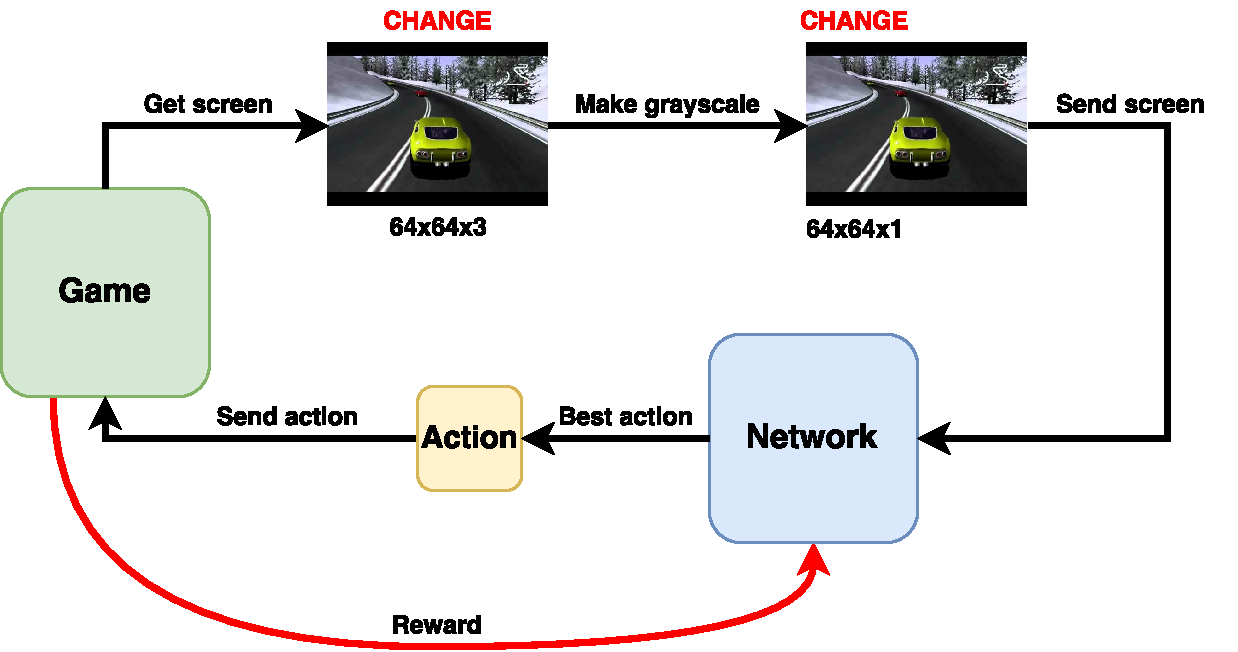
\includegraphics[width=1\textwidth]{Figures/Architecture/TORCS_interaction.pdf}
	\caption{The interaction between the game (TORCS) and the network }
	\label{fig:TORCS_interaction}
\end{figure}

 
As seen on \Cref{fig:TORCS_interaction} the screen is taken from the game, which in this project is TORCS. The screen is the state in our reinforcement learning algorithm. The image screen in this case is of size $64 \times 64$ and have three color channels - red, green and blue. Then some preprocessing is happening for getting this image to the right format, so the network can analyze it. 

 The preprocessing of the image, is to make the image to grayscale. This is done by taken the RGB-image array ($64 \times 64 \times 3$) and separate the 3 color channels red, green and blue. These RGB-values is converted to grayscale values by forming a weighted sum of the R, G and B components:

\begin{equation}
grayscale = 0.2989 \cdot R + 0.5870 \cdot G + 0.1140 \cdot B 
\end{equation}  

The network will then take $64 \times 64 $ image as inputs, more about the network used in this project is described in \Cref{sec:A3C}. The network then uses this input to find the best action, in this state (screen of the game). 

The action the network has found, is then send to the game. The game will then behave after this action and send a reward back to the network. This reward is used to learn the network how to play the game - this is also called training of the network. This procedure continues until the maximum reward is achieved.   
 

 

 
   
\section{Asynchronous Advantage Actor Critic}
The newest breakthrough in RL is the \textit{Asynchronous Advantage Actor Critic} (A3C) approach, and therefore it was chosen to be studied and implemented onto the idea of driver-less cars. In order to achieve a similar environment as the one of a car, and also to be able to get the necessary data easier a car simulator was chosen for the project. Among the existing car simulators encountered in the different online sources, and after analyzing the DDPG implementation on The Open Racing Car Simulator (TORCS) \cite{DDPG_Torcs}, the project settled for this car simulator as well.

The project was mainly inspired from the article \cite{DBLP:journals/corr/MnihBMGLHSK16} summarized in the section \ref{AsyncMeths}, and also from the recent implementation of the A3C into the Doom game elaborated on in \cite{A3CDoom}.

The idea behind the A3C is very much around the same \textit{actor-critic} approach described in the section \ref{PolicyGradMeths}, that more accurately is founded on the presence of both the value function approximator, $\theta_{v}$ and the bootstrapping policy estimator, $\theta$. An additional feature to the actor-critic method is the \textit{asynchronous} part. Instead of having a single agent training on the GPU as in the example of the DDPG project elaborated in the previous section, multiple agents are instantiated for training on different CPU threads simultaneously, and, unlike in the DDPG where there are two different networks, in the A3C the agents share a global network, which is updated as the agents advance. Another new feature of the A3C is the \textit{advantage} element, which is just a mathematical way of expressing how much better some actions ended up to be, and where the estimation should be improved. The update performed by the A3C is of the form $\nabla_{\theta'}\textup{log}\pi(a|s,\theta')A(s,a,\theta,\theta_{v})$, and the formula for the advantage is $\sum_{i=0}^{k-1}\gamma^{i}r_{t+i}+\gamma^kV(s_{t+k},\theta_{v})-V(s_{t},\theta_{v})$, which are both taken from the article \cite{DBLP:journals/corr/MnihBMGLHSK16}. The update formula changes slightly after including the entropy factor in the policy in order to encourage exploration and avoid convergence to an earlier suboptimal solution. The detailed A3C algorithm taken from \cite{DBLP:journals/corr/MnihBMGLHSK16} is listed below.
\begin{algorithm}[H]
	\caption{Asynchronous advantage actor-critic - pseudocode for each actor-learner thread.}
	\label{algo:A3C}
	\begin{algorithmic}
		\State \textit{//Assume global shared parameter vectors $\theta$ and $\theta_{v}$ and counter $T=0$}
		\State \textit{//Assume thread-specific parameter vectors $\theta'$ and $\theta_{v}'$}
		\State Initialize thread step counter $t\leftarrow1$
		\Repeat
		\State Reset gradients: $d\theta\leftarrow 0$ and $d\theta_{v}\leftarrow0$
		\State Synchronize thread-specific parameters $\theta'=\theta$ and $\theta_{v}'=\theta_{v}$
		\State $t_{start}=t$
		\State Get state $s_{t}$
		\Repeat
		\State Perform action $a_{t}$ according to policy $\pi(a_{t}|s_{t}, \theta')$
		\State Receive reward $r_{t}$ and new state $s_{t+1}$
		\State $t\leftarrow t+1$
		\State $T\leftarrow T+1$
		\Until terminal \textbf{or} $t-t_{start}==t_{max}$
		\If {$s_{t}$ is terminal}
		\State $R=0$
		\Else 
		\State $R=V(s_{t},\theta_{v}')$ \textit{//bootstrap from last state }
		\EndIf
		\For {$i \in \left \{ t-1,...,t_{start} \right \}$}
		\State $R\leftarrow r_{i}+\gamma R$
		\State Accumulate gradients wrt $\theta'$:
		\State $d\theta\leftarrow d\theta+\nabla_{\theta'}\textup{log}\pi(a_{i}|s_{i},\theta')(R-V(s_{i},\theta_{v}'))$
		\State Accumulate gradients wrt $\theta_{v}'$:
		\State $d\theta_{v}\leftarrow d\theta_{v} + \partial (R-V(s_{i},\theta_{v}'))^2/ \partial\theta_{v}'$
		\EndFor
		\State Perform asynchronous update of $\theta$ using $d\theta$ and of $\theta_{v}$ using $d\theta_{v}$
		\Until $T>T_{max}$
	\end{algorithmic}
\end{algorithm}

The A3C implementation into the Doom game uses images generated by the vizDoom environment as input data for the well known nonlinear function approximation solution method - ANN. The images become the \textit{states} of the RL problem based on which the AI agent learns to shoot the opponents. The vizDoom environment has a \textit{reward} function predefined, which is triggered when the agent deploys an action in the environment. As the given implementation was made for the \textit{discrete actions space}, the estimated policy or the \textit{actor} provides the probabilities of taking each action in a specific state, and so, in each state the action with the maximal probability is chosen to be pursued. The \textit{critic}, on the other hand, estimates a state-value function for the existing policy and it is used in the composition of the loss function, which represents the performance measure or the \textit{objective function} of the RL problem.

The A3C project developed for the TORCS environment has the same principles as the A3C Doom. It also uses images as the input states into a deep ANN structure and the mathematical model of the problem is similar. The TORCS environment is more flexible and that is an advantage as it offers more freedom for changing things and get better results. For example, it is easier to change the reward function and perform action manipulations, and this will be further explained and illustrated in the next chapter. Another additional implementation is the \textit{continuous} actions space, which is slightly different than the \textit{discrete} actions space implementation; nevertheless they were both preserved in the project for analysis purposes. The structure of the deep ANN will offer more insight on how the program works. Therefore, the overall structure of the ANN of the A3C TORCS project is presented in the following figure:
\begin{figure}[H]
	\centering
	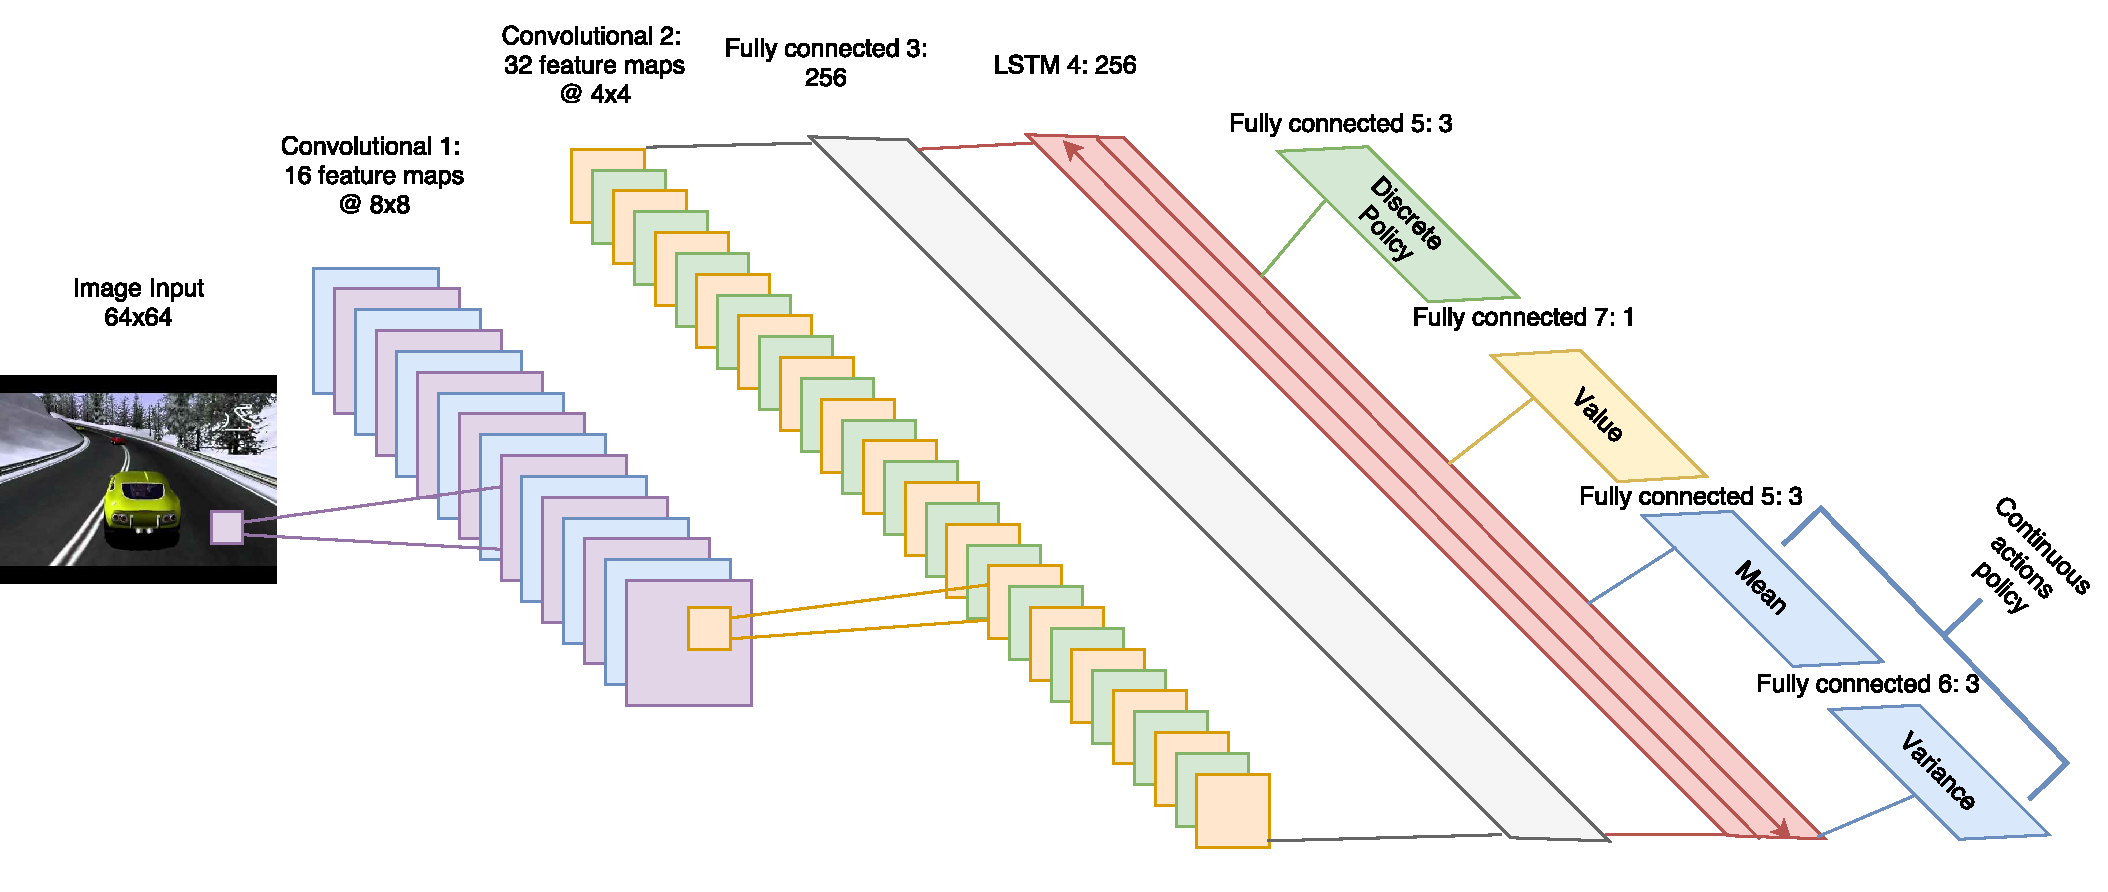
\includegraphics[width=1.25\textwidth]{Figures/A3CTorcs}
	\caption{The ANN structure of the A3C implementation into Torcs}
	\label{A3CTorcs}
\end{figure}
The image of size 64x64 comes into the ANN as input and goes through the first layer of ANN - a convolutional layer that outputs 16 feature maps of sizes 8x8 each. Next, these are again passed through another convolutional layer that outputs 32 feature maps of size 4x4 each, while taking care of spatial correlations. Then the output is flattened with a fully connected layer and passed to a recurrent layer - basic LSTM, that takes care of the temporal dependencies. Finally, the output of the LSTM layer can be used for the last layers of the ANN. The value function is linearly estimated, while the discrete policy is estimated with a softmax activation function and gives the probabilities of each action in the discrete set. For the continuous actions space, on the other hand, the discrete policy is replaced by 2 other layers that estimate the mean $\mu$ and the variance $\sigma$ which form a normal distribution. The formed normal distribution is then sampled to get the action to be passed to the environment.

The flow of the program is as follows. First, a global network is defined and a number of agents or workers are instantiated to train themselves in their own environment using a copy of the global network. During training, as the first state of the environment is received and passed through all the ANN layers, the worker picks the action with the highest probability given by the output of the discrete policy layer, and then the worker executes the action while the environment returns the next state and the reward. The states keep coming during an episode and the rewards keep accumulating together with the values in an episode buffer. At every step the global network is being updated with the data from the episode buffer, and when the buffer is full, then the network bootstraps from the current value estimate to update the whole network. The update of the global network happens by applying gradients that were computed for a defined loss function. A very general illustration of the flow of the program is shown below.
\begin{figure}[H]
	\centering
	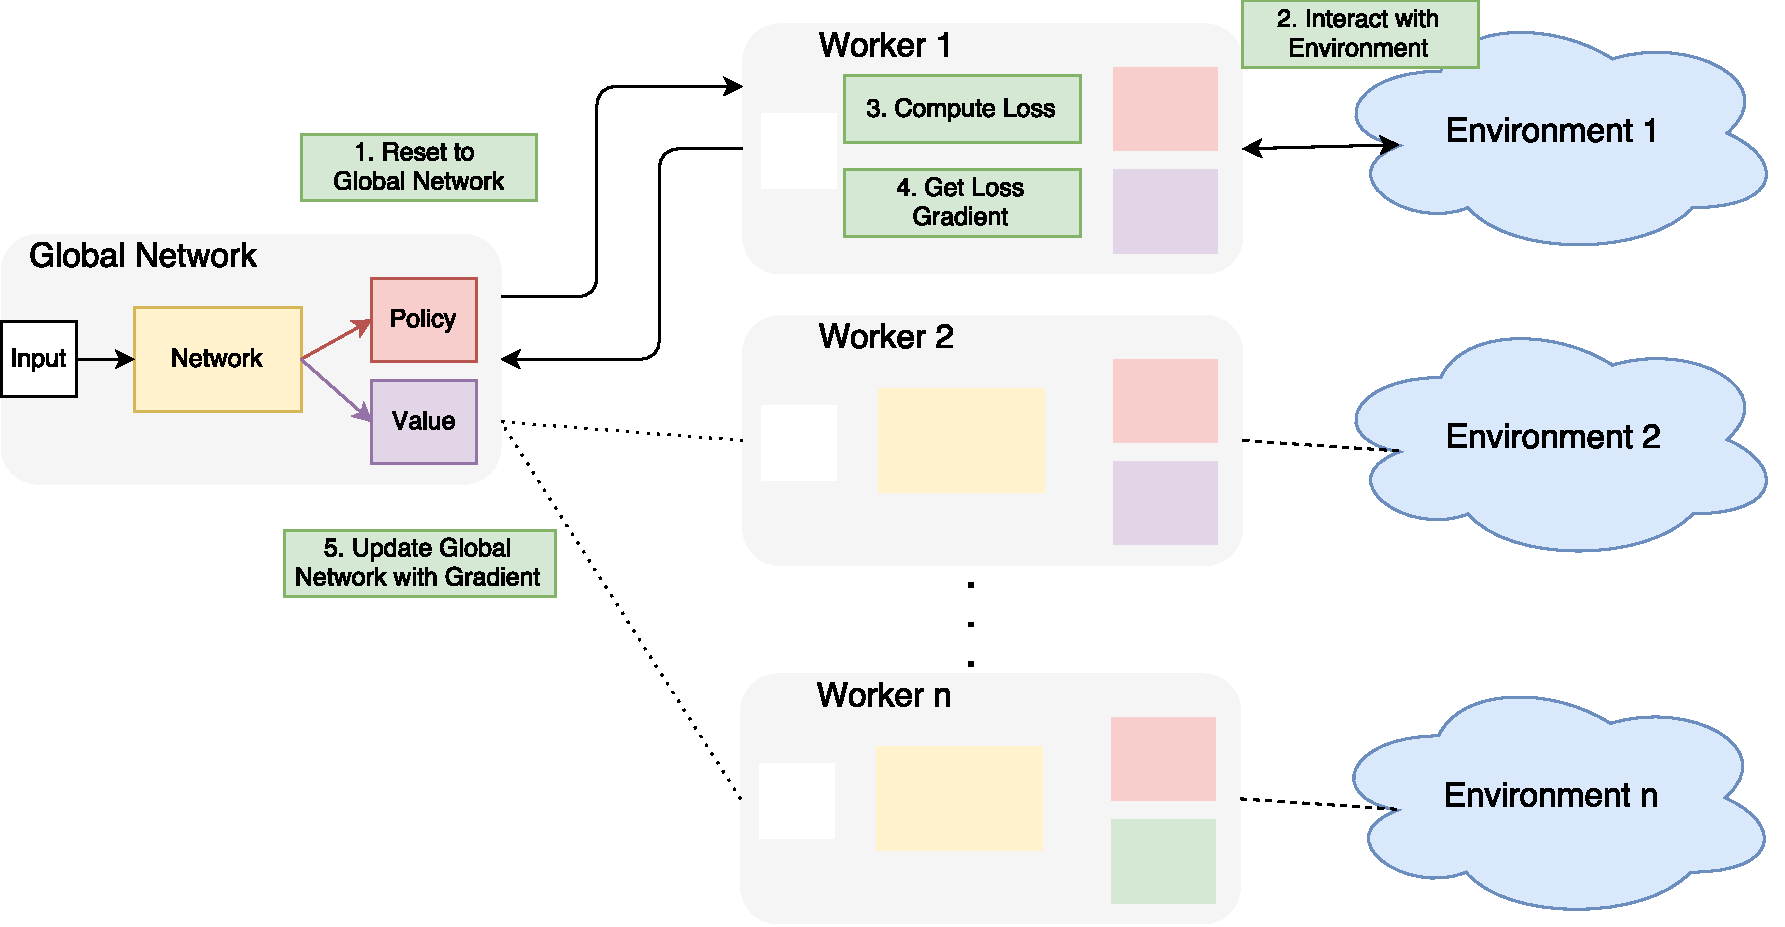
\includegraphics[width=1.25\textwidth]{Figures/Flow}
	\caption{The flow of the A3C Torcs program}
	\label{Flow}
\end{figure}
The loss function is composed of the value loss, policy loss and the entropy loss. Each of these are assigned specific weights that they would have in the total loss result. This loss function represents the performance measure of the problem, the goal, or the objective function. The gradient of the loss function with respect to the weights of the ANN are calculated and applied using an optimizer. The recommended optimizers are RMSProp and, an evolved form of it - the Adam optimizer. The learning rate for these is 1e-4. The discount factor used for the RL problem stated is 0.99.
\chapter{Results}
\label{cha:Result}
The project code is provided in the public GitHub repository at the following link: https://github.com/popovicidaniela/Master-Thesis.
The A3C-Torcs can be run and tested with the generated tensorboard graphs.

For monitoring and understanding better the training process, some performance and loss measures were taken into account in generating graphs in tensorboard. The measures are added to a tf.Summary(), which then is added to a tf.summary.FileWriter() in order to make the data accessible in the tensorboard.

The relevant performance measures are the length of the episode, accumulated reward, and the value function result. These values should be growing. The length of the episode grows until the agent has been trained to drive the whole lap. The more the car stays in the game and the better it drives, the more reward it gets and the better value function results. If the car crashes then the length of the episode is short, and because it is learning, the graph should show an increasing curve as the training advances. 

The loss measures are the ones that participate in the composition of the loss function. These include policy, value, and entropy losses. These results should show decreasing curves as the loss is being minimized with each step and the estimations become more accurate. The entropy is representing the amount of exploration that the agent is making, the more it learns, the less it explores, therefore the entropy is decreasing, and the agent acts more and more based on his knowledge as it progresses.

The following figures present the results of training using A3C for 4 workers in parallel, the Adam optimizer with the learning rate of $10^{-4}$. Figure \ref{fig:RewardHours} shows the accumulated reward after hours of training, whereas y-axis represents the accumulated reward and x-axis - the hours of training. The values plotted on all graphs are the values accumulated over each 5 episodes, where an episode terminates when the car goes out of the track or when the car finishes a lap. In each episode, there are a certain number of state (images or frames) and action pairs. Figure \ref{fig:Length} plots the mean accumulated length of an episode in terms of the number of states that the car has been into in the last 5 episodes. For this figure and the rest of them, the x-axis is expressed in time-steps, where a time-step is the mean accumulated values over 5 episodes.

\begin{figure}[H]
	\advance\leftskip-4cm
	\minipage{0.7\textwidth}
	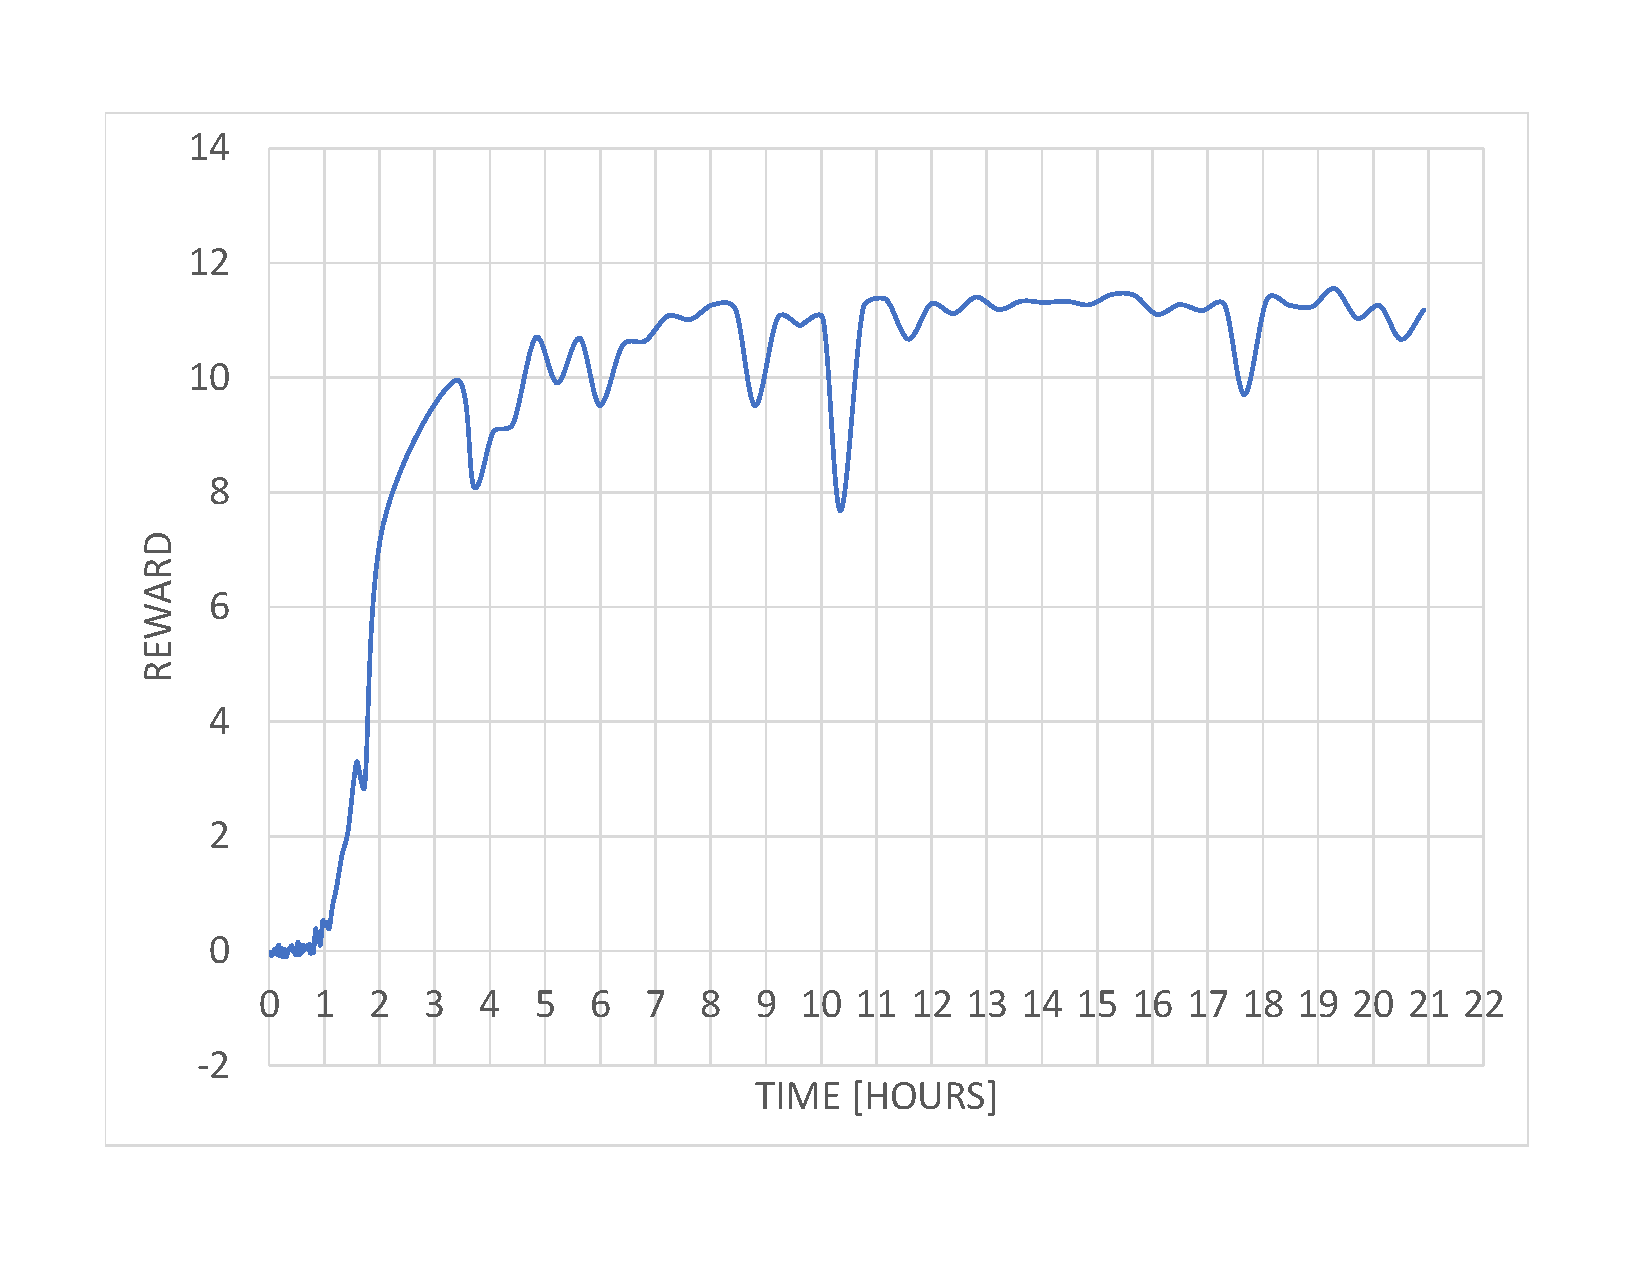
\includegraphics[width=\linewidth]{Figures/Result/reward_in_hours_best.pdf}
	\caption{Reward in Hours on the x-axis}\label{fig:RewardHours}
	\endminipage\hfill
	\minipage{0.7\textwidth}
	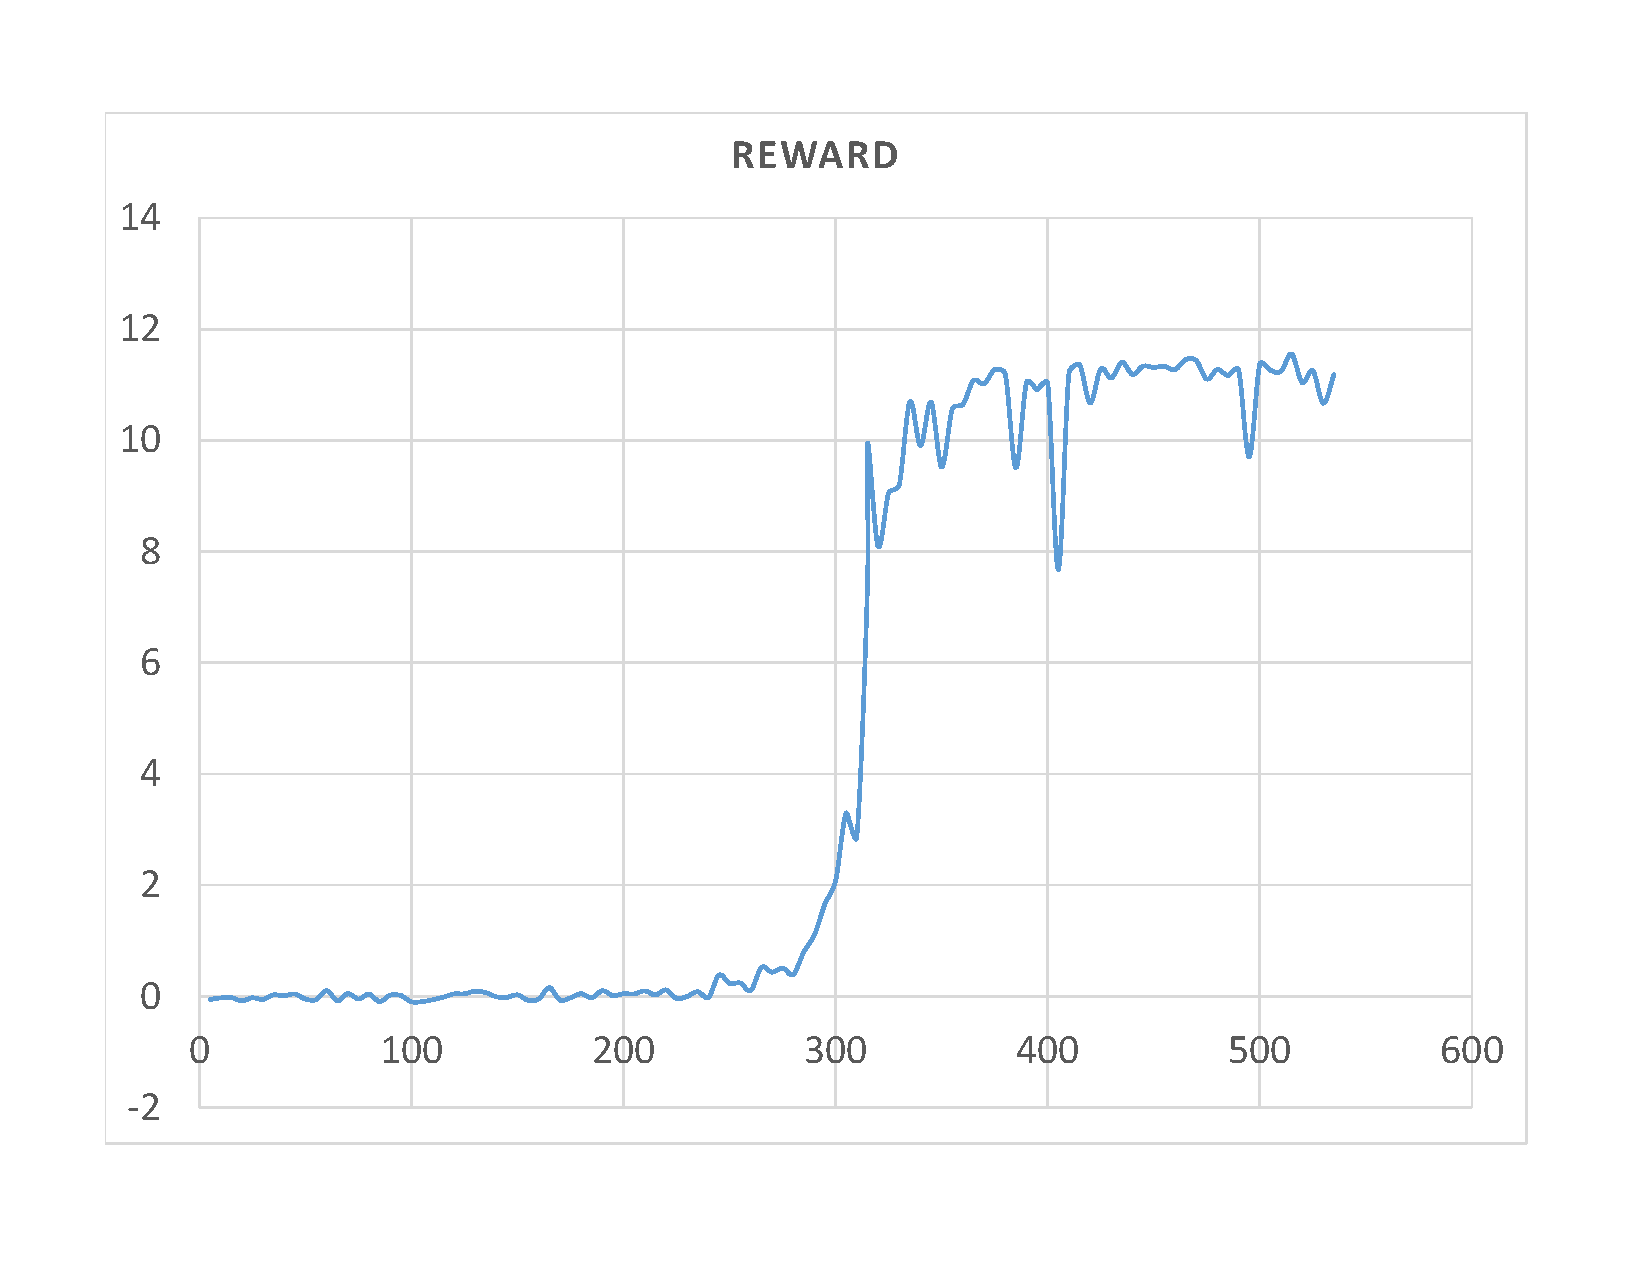
\includegraphics[width=\textwidth]{Figures/Reward}
	\caption{Reward}
	\label{fig:Reward}
	\endminipage
\end{figure}
\begin{figure}[H]
	\advance\leftskip-4cm
	\minipage{0.7\textwidth}
	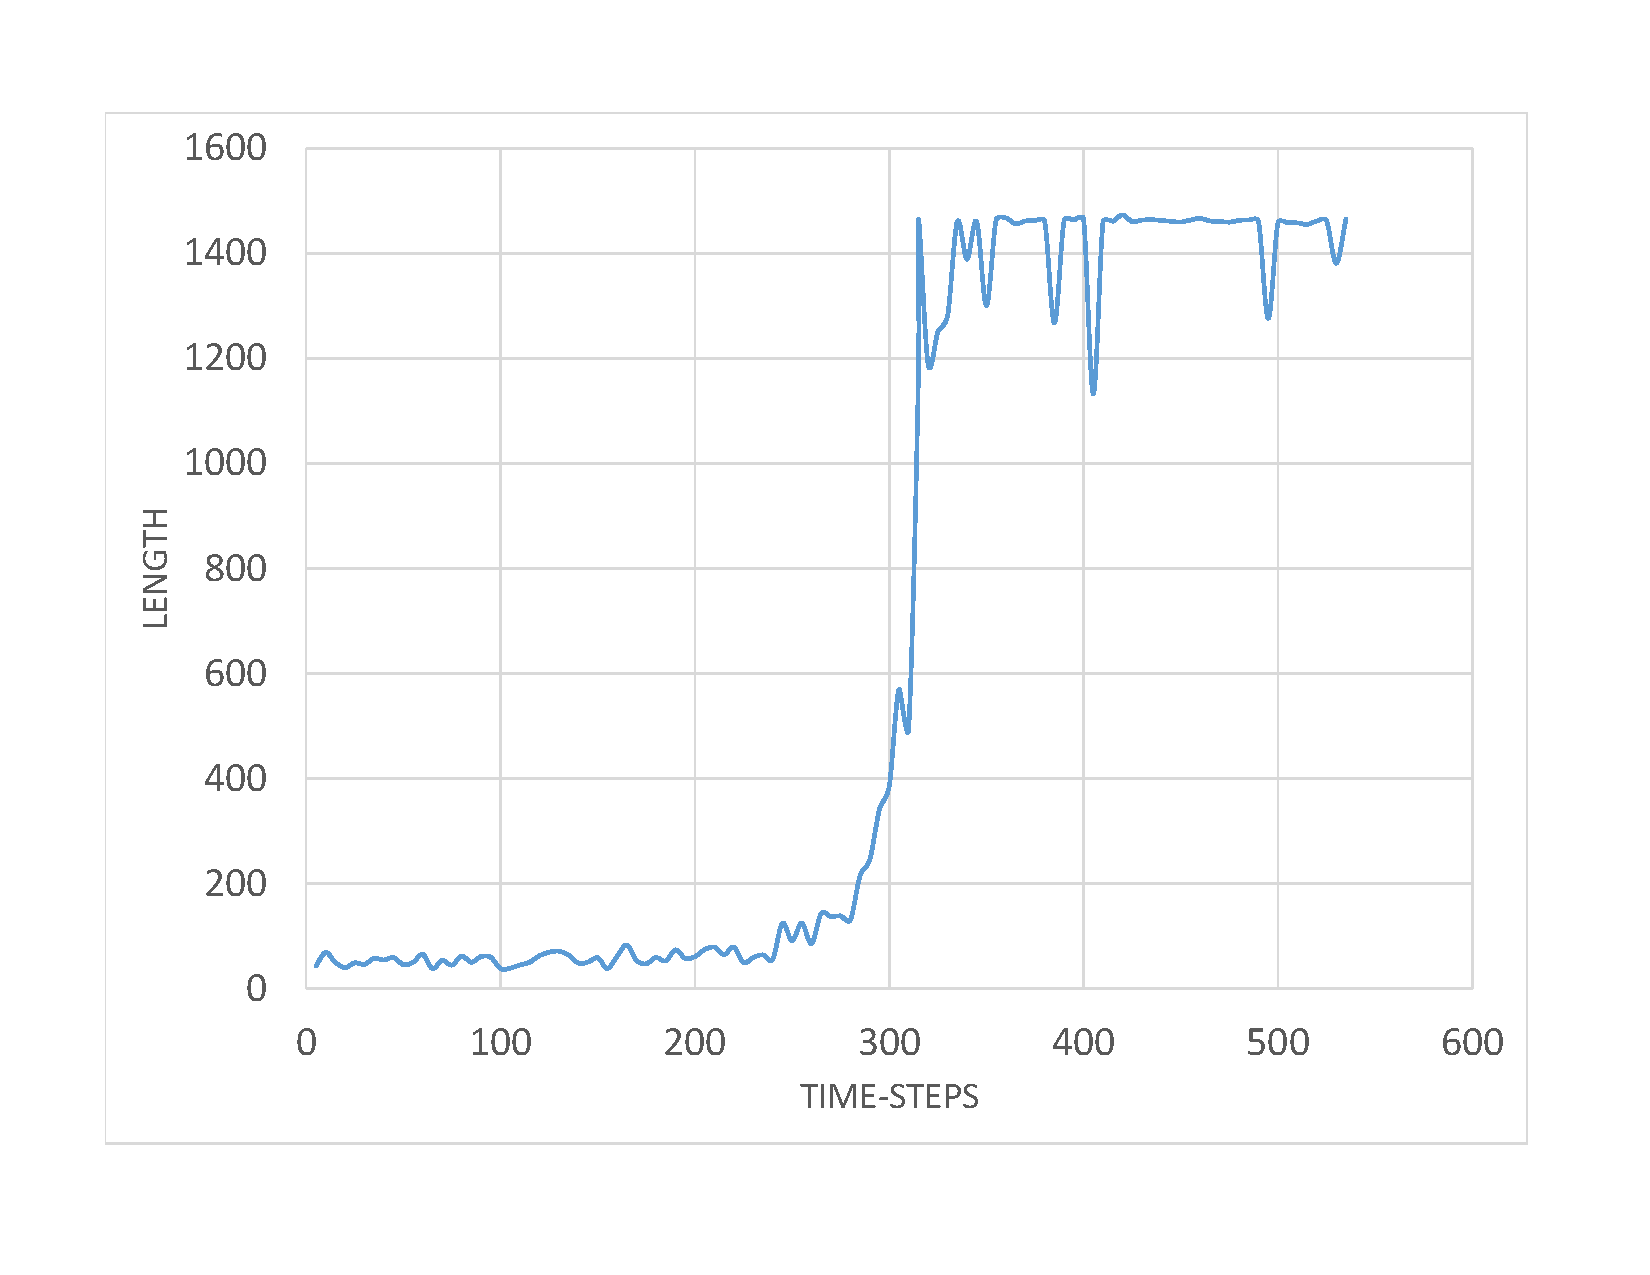
\includegraphics[width=\linewidth]{Figures/Length}
	\caption{Length}\label{fig:Length}
	\endminipage\hfill
	\minipage{0.7\textwidth}
	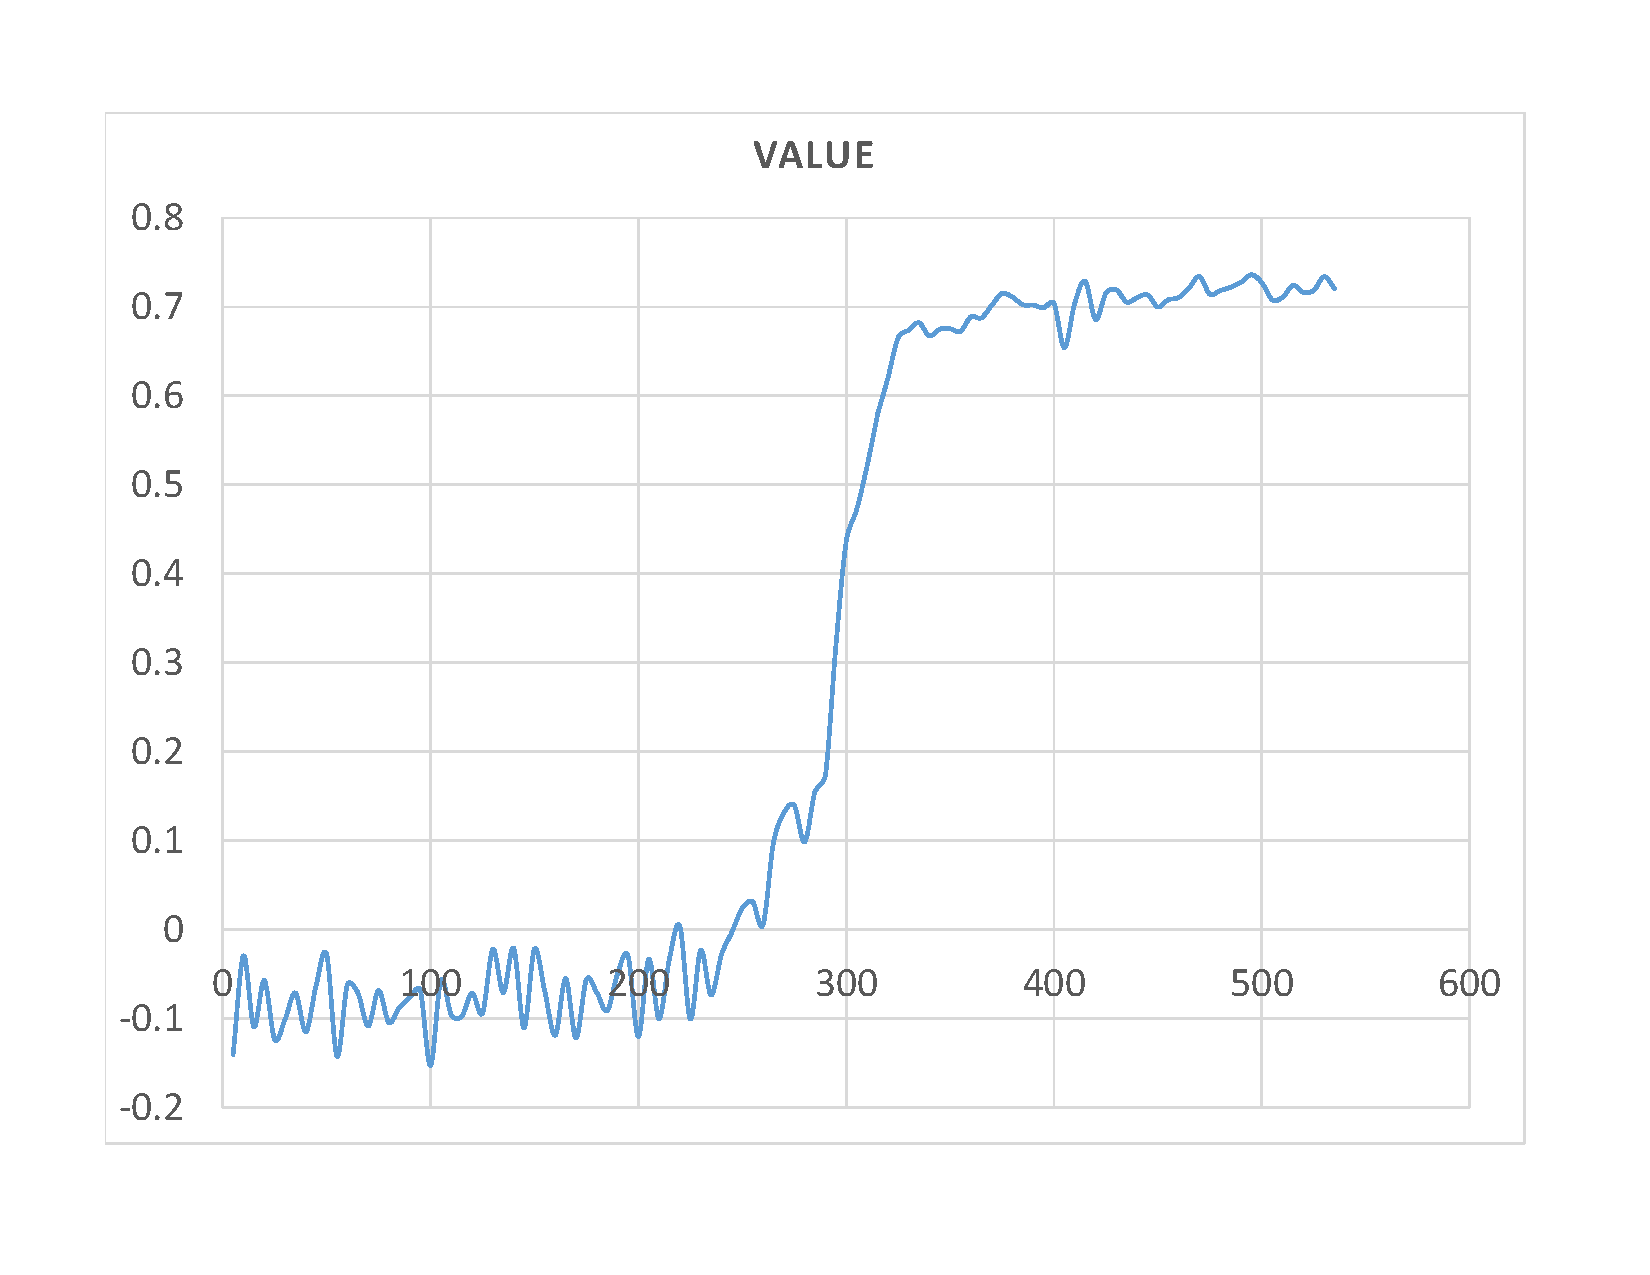
\includegraphics[width=\textwidth]{Figures/Value}
	\caption{Value}
	\label{fig:Value}
	\endminipage
\end{figure}
\begin{figure}[H]
	\advance\leftskip-2cm
	\minipage{0.7\textwidth}
	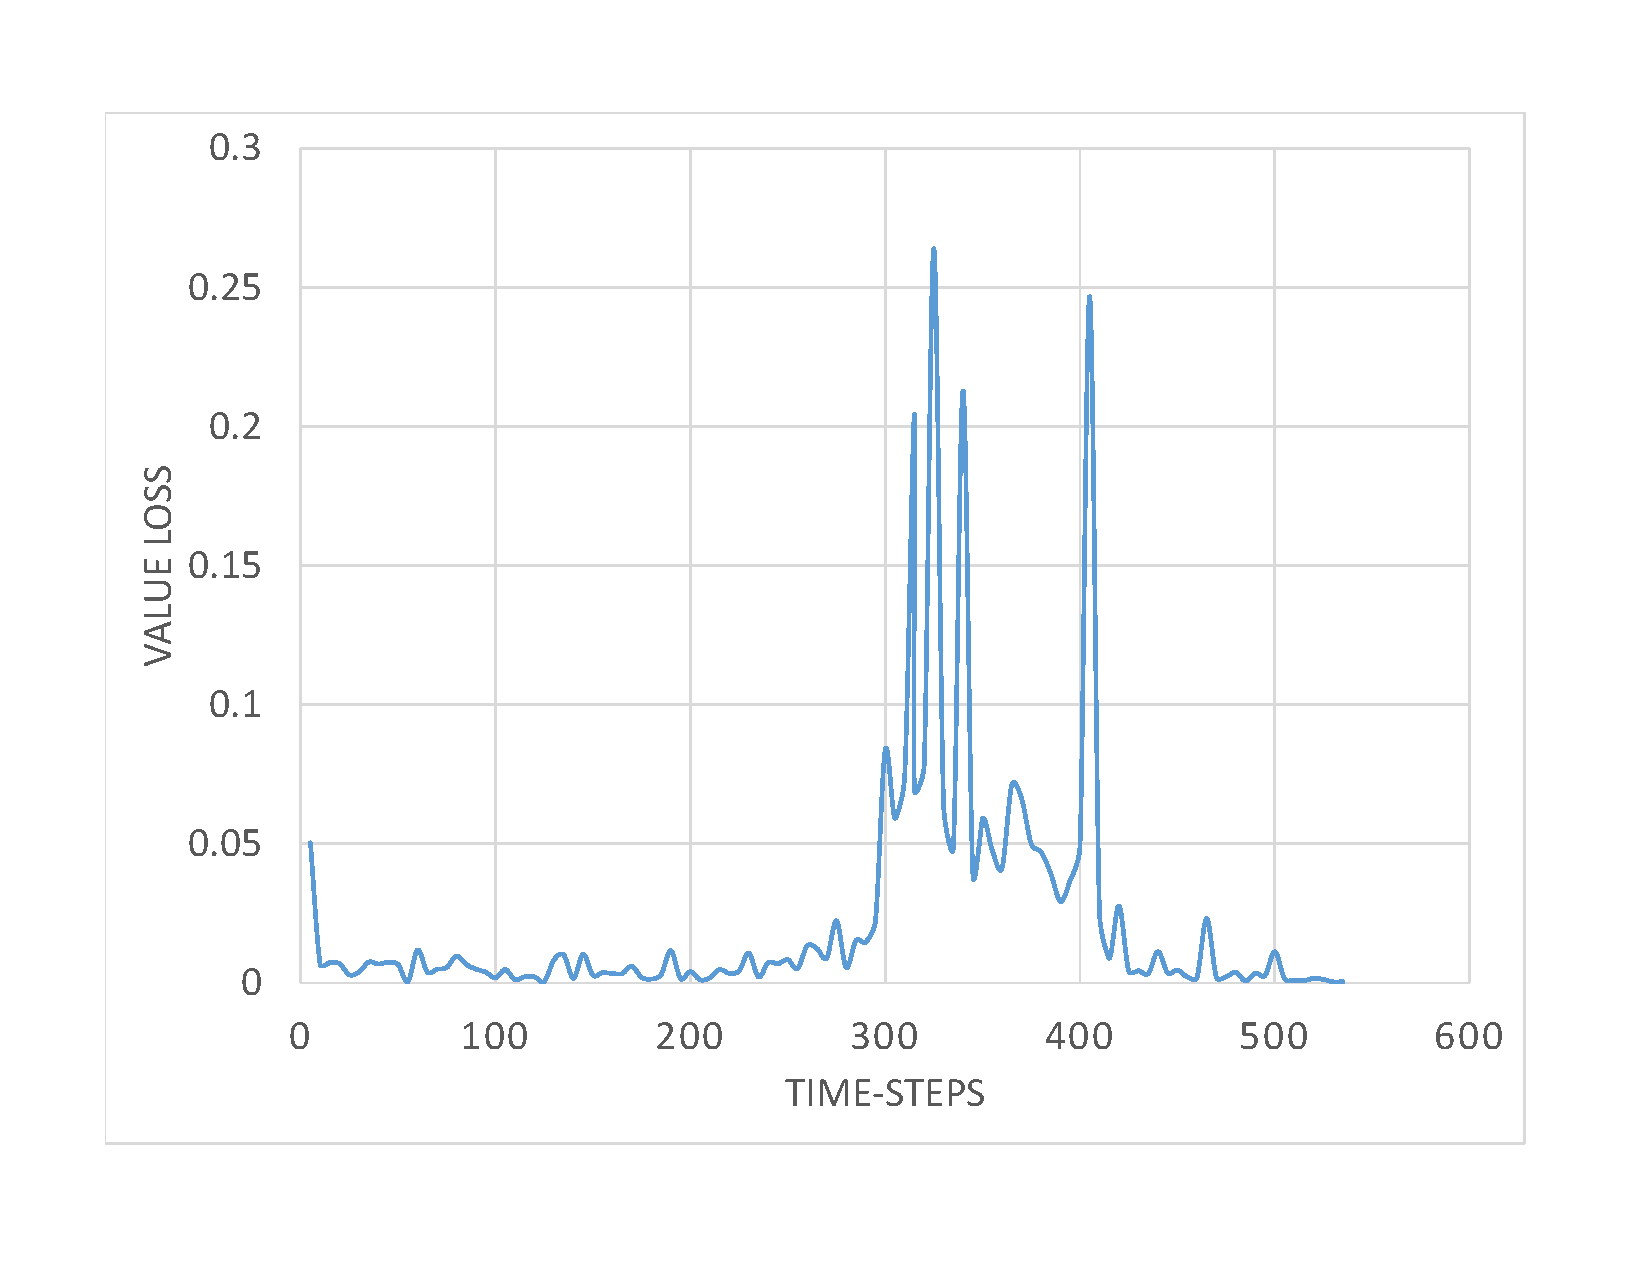
\includegraphics[width=\linewidth]{Figures/ValueLoss}
	\caption{Value Loss}\label{fig:ValueLoss}
	\endminipage\hfill
	\minipage{0.7\textwidth}
	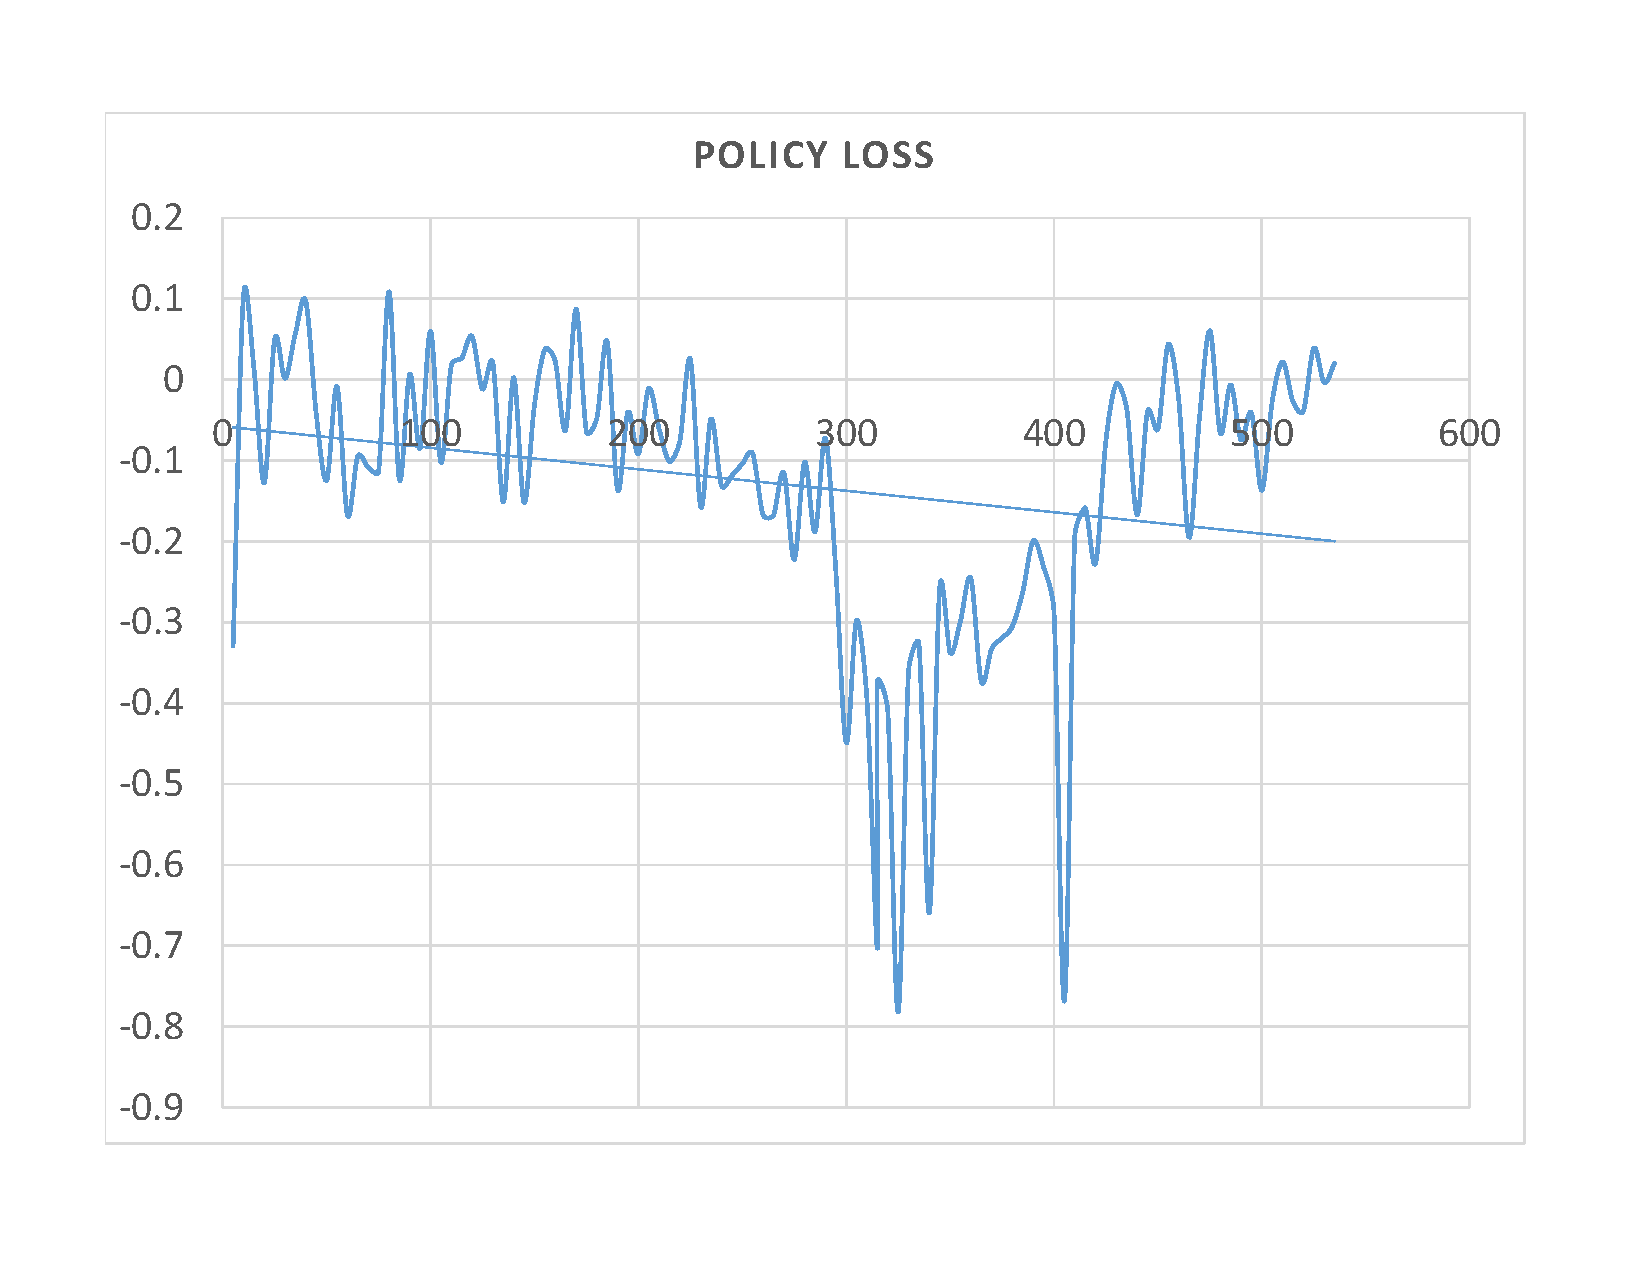
\includegraphics[width=\textwidth]{Figures/PolicyLoss}
	\caption{Policy Loss}
	\label{fig:PolicyLoss}
	\endminipage
\end{figure}
\begin{figure}[H]
	\advance\leftskip-2cm
	\minipage{0.7\textwidth}
	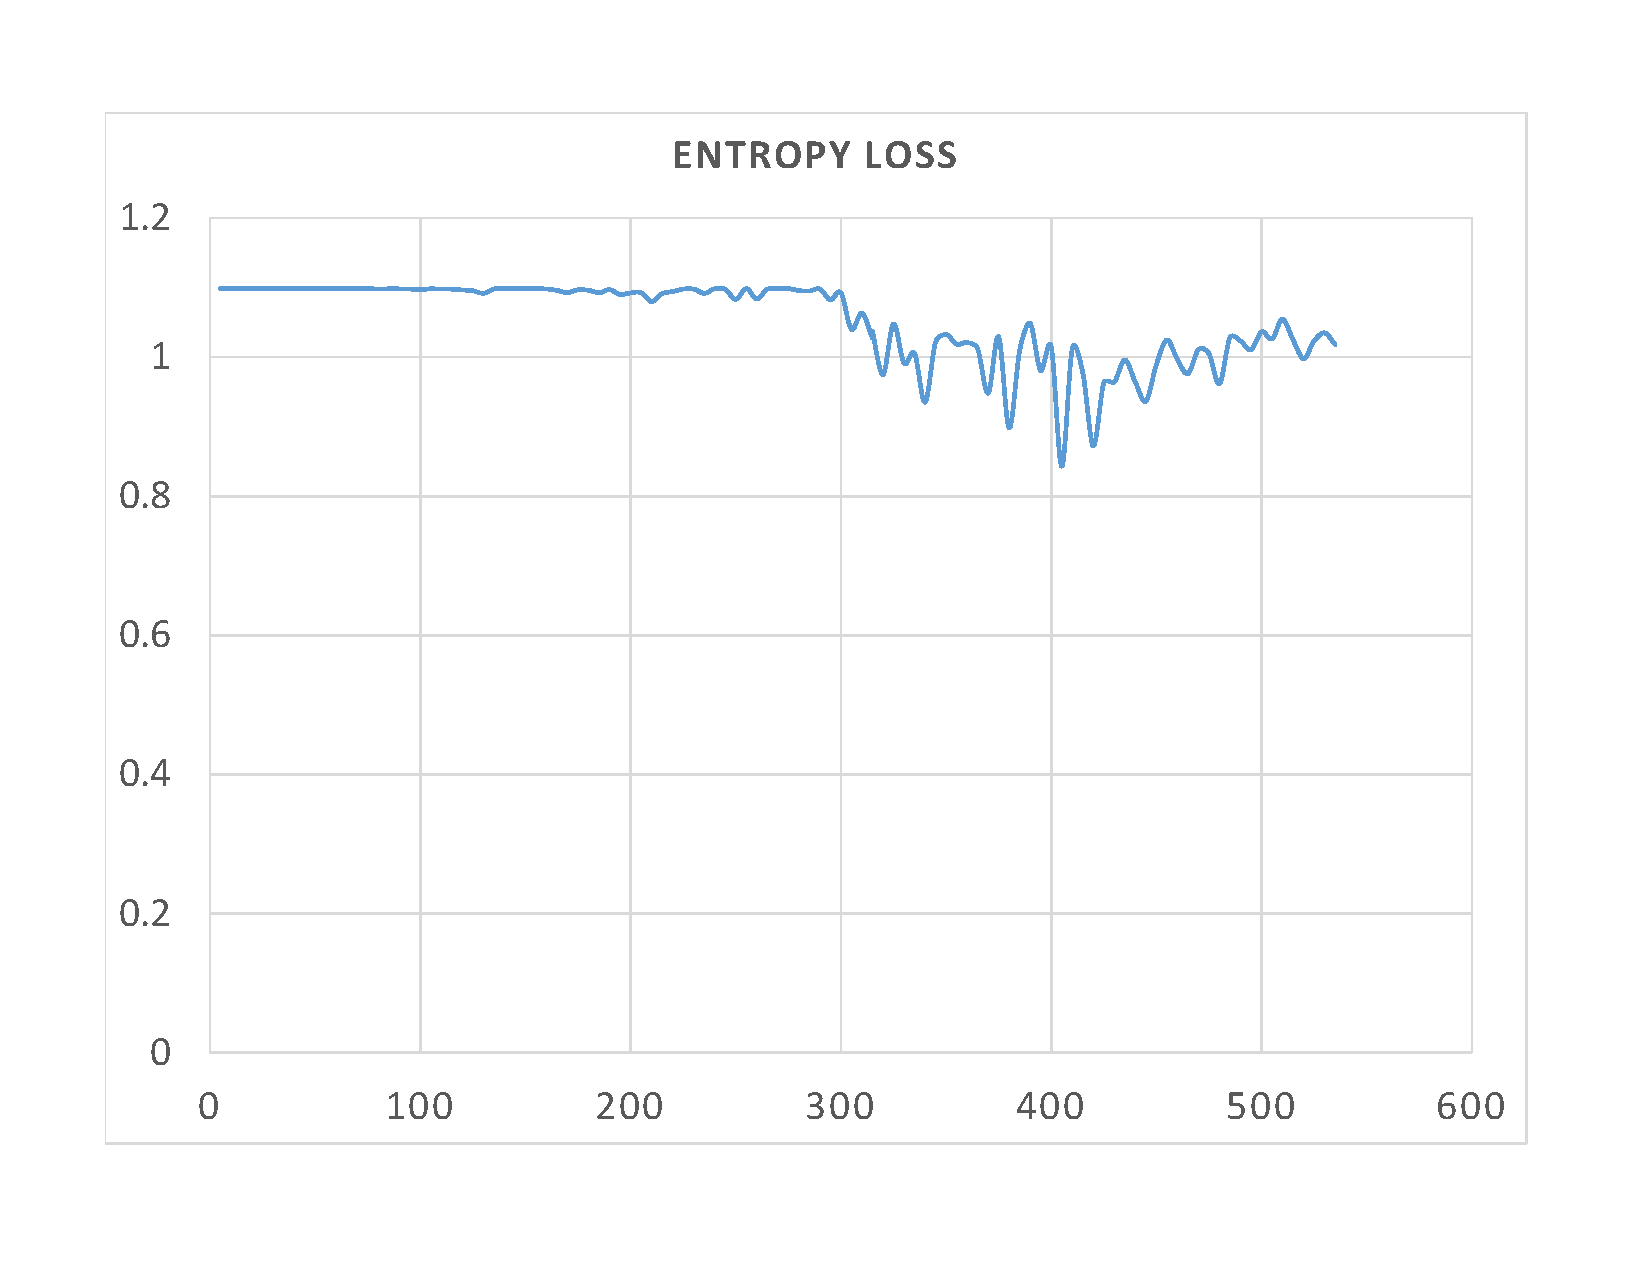
\includegraphics[width=\linewidth]{Figures/EntropyLoss}
	\caption{Entropy Loss}\label{fig:EntropyLoss}
	\endminipage\hfill
	\minipage{0.7\textwidth}
	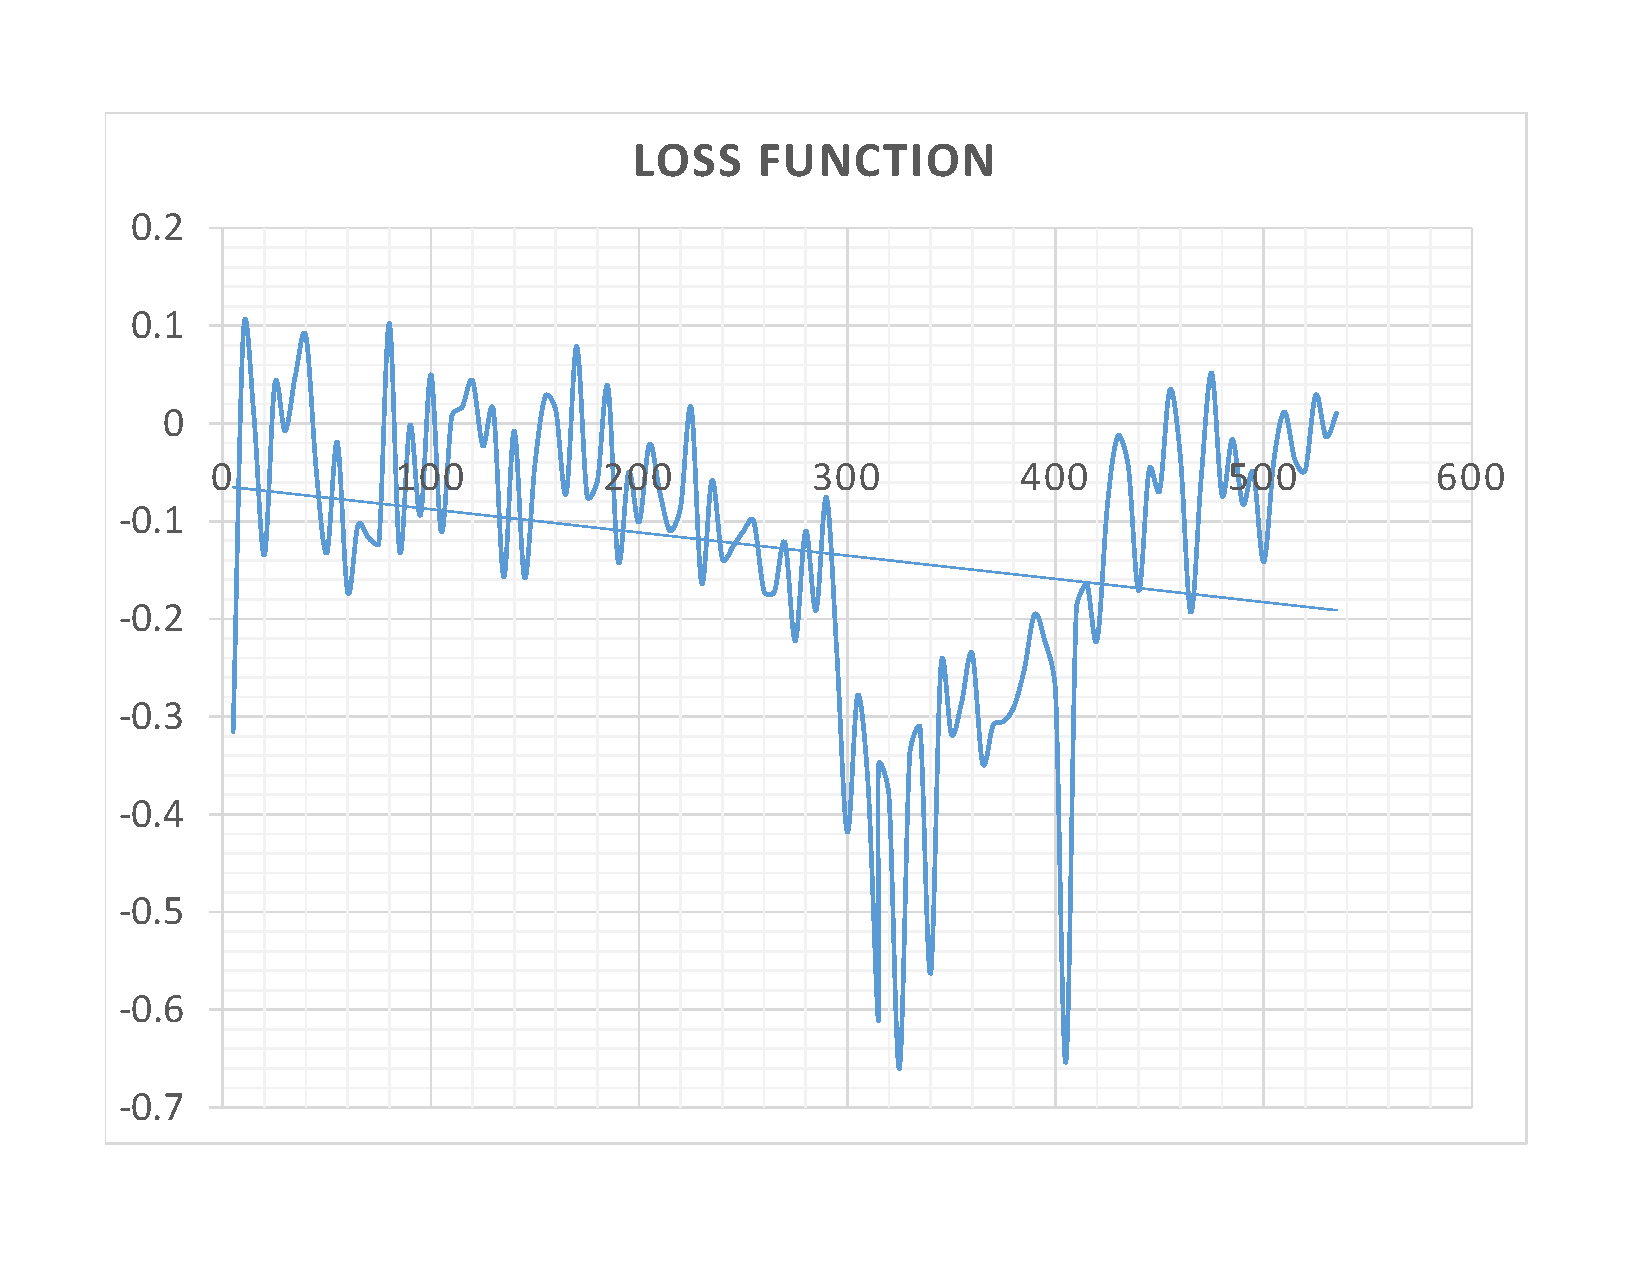
\includegraphics[width=\linewidth]{Figures/Loss}
	\caption{Loss}\label{fig:Loss}
	\endminipage
\end{figure}
As we can see from the figures the training has finished when the agent learned to drive the whole lap and the monotonicity of the plotted curves are as expected (as described above). After $5-6$ hours ($300$ time-steps) of training the values started to converge. The trained agent was played on different tracks to test that it learned to drive, but more about this in the section about the different tracks in \Cref{Tracks}.

The chapter continues with presenting the different scenarios that offer insights in performance and environment manipulations. More precisely, the performance of two different optimizers will be compared, the scenarios with a different number of workers will be presented, and different action spaces. The environment specific experiments list some manipulations with the reward function, speed, acceleration and playing the trained agent on other tracks, too.

%network
\section{Optimizers}
It was mentioned at the end of the previous chapter that the recommended optimizers were RMSProp and Adam. RMSProp was used in the experimental set-ups of the Atari games in \cite{DBLP:journals/corr/MnihKSGAWR13} and TORCS in \cite{DBLP:journals/corr/MnihBMGLHSK16}. Also, RMSProp was mentioned in section \ref{RNN} as a solution for the vanishing and exploding gradients problems in RNNs. The Adam optimizer was more often found in the working examples online: in the DDPG for TORCS \cite{DDPG_Torcs}, and in the A3C for Doom \cite{A3CDoom}.

RMSProp and Adam algorithms are extensions of the basic SGD (described in the section \ref{Approximate solution methods}). The problem of identifying a learning rate persists, as it is well known that a too low learning rate results in slow training, whereas a too big learning rate would cause a lot of noise in the objective function so that it would never converge. These SGD extensions try to solve the learning rate problem by adapting it for each of the parameters. 

RMSProp's "idea is to divide the learning rate for a weight by a running average of the magnitudes of recent gradients for that weight" \cite{RMSProp}. The update formula is given by \cite{DBLP:journals/corr/MnihBMGLHSK16}:
\begin{equation}\label{RMSPropUpdate}
\begin{aligned}
g&=\alpha g + (1-\alpha)\Delta \theta^2\\
\theta & \leftarrow \theta - \eta  \frac{\Delta \theta}{\sqrt{g+\epsilon}},
\end{aligned}
\end{equation}
where $\theta$ represents the weights shared across all threads, $\Delta \theta$ is the accumulated gradients of the loss with respect to the $\theta$, $\eta$ is the learning rate, $\alpha$ is the momentum that keeps knowledge of the previous experience, and $g$ is "the moving average of element-wise squared gradients" \cite{DBLP:journals/corr/MnihBMGLHSK16}.

Adam optimizer's principles are a lot like those of RMSProp. Adam algorithm not only keeps the second order moments $g_{t}$, but it also keeps the first order moments $m_{t}$ of the gradients, which are both decayed over time \cite{Optimizers}. The corresponding formulas are listed below:
\begin{equation}\label{Adam}
\begin{aligned}
m_{t+1}&=\alpha_{1} m_{t} + (1-\alpha_{1})\Delta \theta\\
g_{t+1}&=\alpha_{2} g_{t} + (1-\alpha_{2})\Delta \theta^2\\
\hat{m}_{t+1}&=\frac{m_{t+1}}{1-\alpha_{1}^{t+1}}  \\
\hat{g}_{t+1}&=\frac{g_{t+1}}{1-\alpha_{2}^{t+1}}  \\
\theta \leftarrow & \theta - \eta  \frac{\hat{m}_{t+1}}{\sqrt{\hat{g}_{t+1}+\epsilon}}
\end{aligned}
\end{equation}

According to the paper \cite{DBLP:journals/corr/MnihBMGLHSK16}, for the asynchronous deep RL methods like the case of A3C, the RMSProp optimizer with shared weights between threads is more robust and also reduces memory requirements than per-thread weights method. So, shared statistics were used for all the scenarios.

Both RMSProp and Adam optimizers are available in the tensorflow library, and, therefore, were easily tried out and analyzed for the current project, A3C TORCS. A comparison of the two optimizers will be elaborated next, based on the tensorboard graphs generated while training the ANN.
\section{Multi-threading}\label{Multi-threading}
The asynchronous part of the A3C algorithm implies a multiplicity of agents trained simultaneously. The different workers share a global network, but train in separate environments. This means that each worker interacts with its own environment, which is a track he is running on. The worker drives the car in a specified track until it crashes, and another frame starts. In such a way, the workers get to explore more of the same track, while incrementally updating a global shared network. This global network is used and continually updated by all the training workers. This facilitates the process of training in a faster tempo because every worker improves the most recent version of the global network.

The global actor-critic network (ACNetwork) is first declared before the workers. Tensorfow has special dedicated methods for enabling multi-threading, which is the Coordinator. The workers are declared and initialized, after which each of them is assigned to a Thread, where they are started to run their own ACNetwork. The multi-threading process is stopped with join() method when all the workers finished their work.

The following figure shows how much faster the training results to be as the number of parallel workers increases. It was chosen to show the performance of accumulating rewards with 1, 4, and  6 workers training in parallel.
\begin{figure}[H]
	\centering
	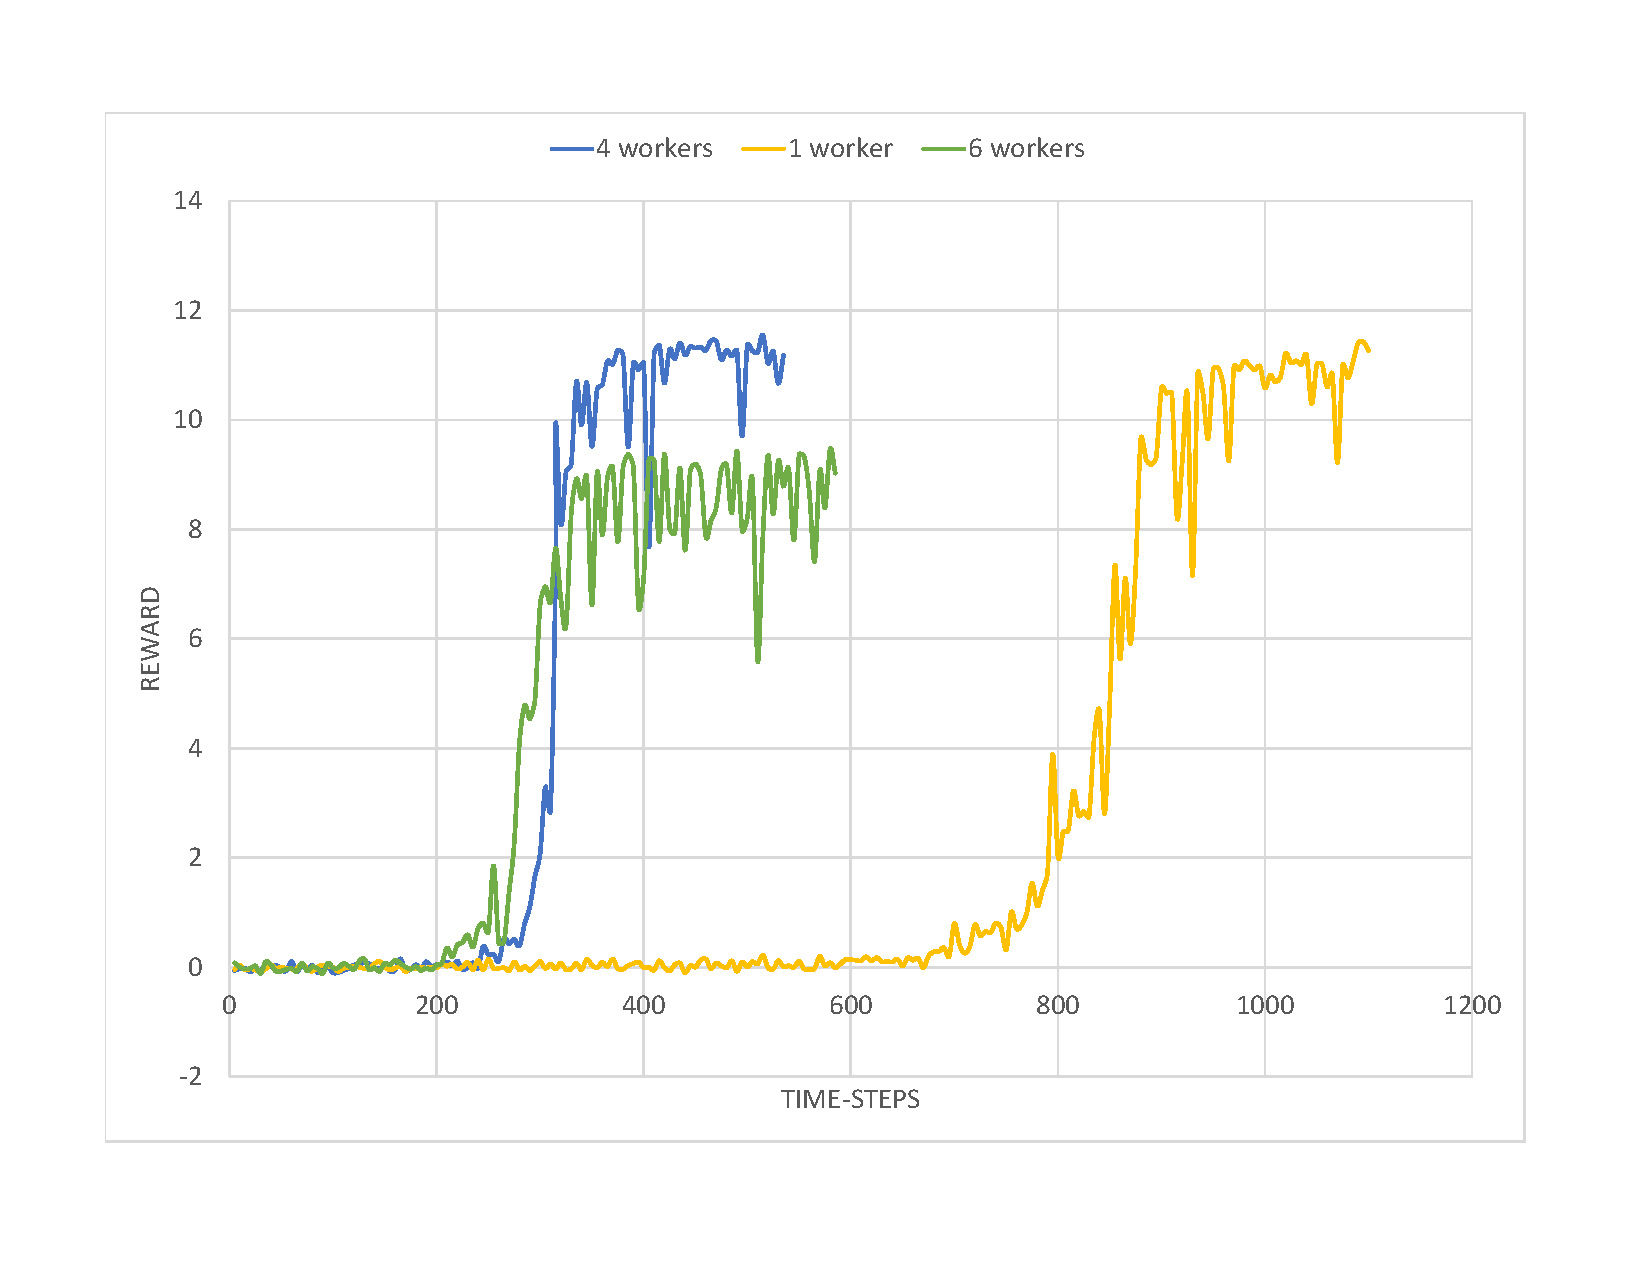
\includegraphics[width=\textwidth]{Figures/Workers}
	\caption{Performance comparison of 1, 4, and 6 workers in parallel}
	\label{fig:Workers}
\end{figure}
 The Figure \ref{fig:Workers} emphasizes that the more workers are used in parallel, the faster the training process becomes. So, for a single worker training alone, the convergence started after 900 time-steps. For 4 workers - the reward function started to grow fast after 250 time-steps, resulting in convergence after 300 time-steps. By increasing the number of workers from 1 to 4, the training became 3 times faster.
 
 It is also possible to see that the training with 6 workers converged to a lower accumulated reward than those of 1 and 4 workers. This is possibly due to a problem of multi-threading the TORCS environment. There are some "Time-out" problems when increasing the number of workers and the performance of the 6 workers was probably affected by it.
\section{Continuous and Discrete Actions Spaces}

\subsection{Discrete Actions Space}

\subsection{Continuous Actions Space}

%environment
\section{Reward}\label{sectionReward}
The reward is really important in reinforcement learning, because it is the one that the agent has to maximize for learning the agent how to act in the environment. For example, consider teaching a dog a new trick: you cannot tell it what to do, but you can reward/punish it if it does the right/wrong thing. It has to figure out what it did that made it get the reward/punishment, which is known as the credit assignment problem \cite{reward_small}. We can use a similar method to train the agent how to drive a car. More about the reward can be read in \Cref{TheorBkgdRL}. 
	
In this project two reward function is compared, for learning the agent how to drive a car in the TORCS environment.  

\subsection*{First reward function}
The first reward function used in this project is the reward function from the paper \cite{DBLP:journals/corr/LillicrapHPHETS15}: \\
\textit{"For the Torcs environment we used a reward function which provides a positive reward each step for the velocity of the car projected along the direction and a penalty of -1 for collisions. Episodes were terminated if progress was not made along the track after 500 frames."}\\
To understand this a figure to illustrate the reward can be seen on \Cref{fig:Reward_paper}.

\begin{figure}[H]
	\centering
	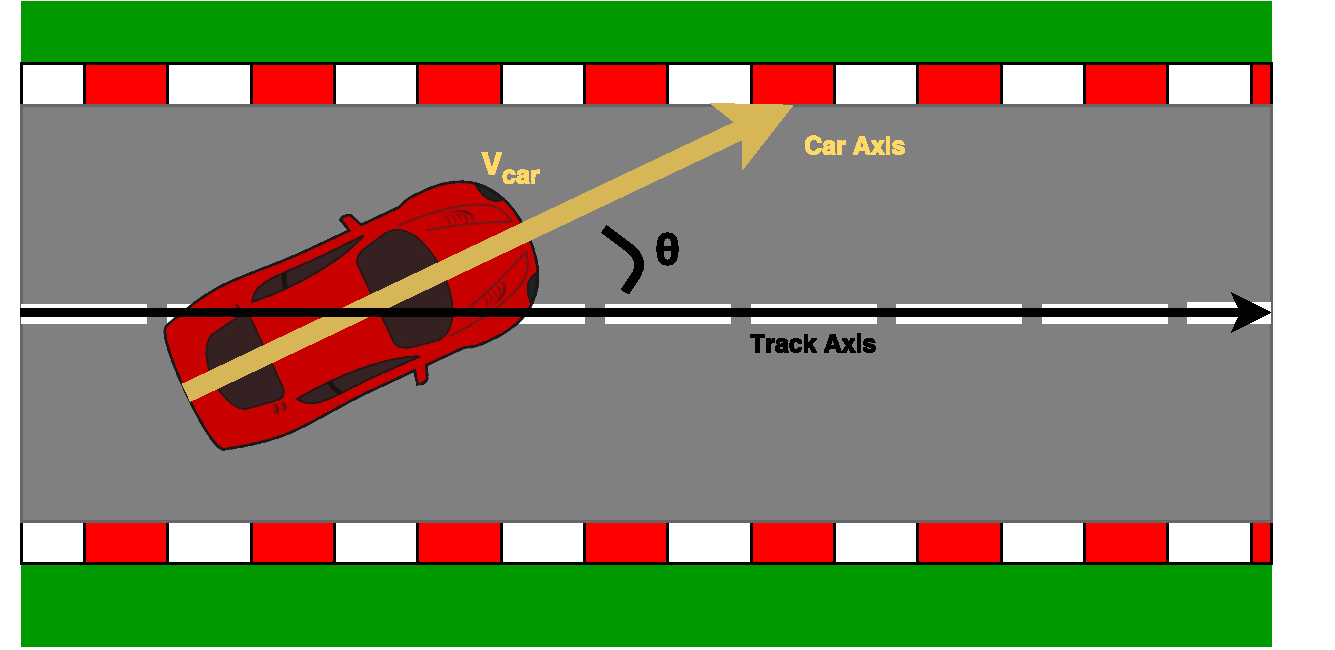
\includegraphics[width=1\textwidth]{Figures/Result/Reward_paper.pdf}
	\caption{Explanation of the reward used in the paper \cite{DBLP:journals/corr/LillicrapHPHETS15} }
	\label{fig:Reward_paper}
\end{figure}

The reward function is then:
\begin{equation}
Reward = V_{car} \cdot cos(\theta) 
\end{equation}
The idea this reward function uses are getting an reward for how fast the car drives in the center of the track. The agent gets more reward, when the car is driving fast at the center of the track, and less reward when the car is driving fast away from the center of the track. 

\subsection*{Second reward function}
After using the first reward function it was concluded that this reward function didn't perform as expected. Because the reward function is important for learning, another reward function is tried. This reward function is taken from the blog \cite{DDPG_Torcs}. Here it uses the same idea, that the reward should be bigger if the car drives fast in the center of the track, and less reward when it is far away from the center. The reward function looks like this:

\begin{equation}
Reward = V_{car} \cdot cos(\theta) - V_{car} \cdot sin(\theta) - V_{car} \cdot \mid trackPos\mid 
\end{equation}
The TrackPos gives percent the car is off center of track. Which is useful in this reward function, when it is wished the car is near the center.  

In this equation the first term want to maximum longitudinal velocity, second term try to minimize transverse velocity, and then it also penalize the AI if it constantly drives very off center of the track in the third term.

Here we see the agent learns how to drive, and this is the reward function where the best results came in this project. It improves the stability of the training.

To test the two reward functions influence on the agent learning, all other parameters stays as described in the introduction to this \Cref{cha:Result}. Thereby it should be possible to only see the influence of the two different reward functions.

To compare both reward functions a graph is created, this graph can be seen on \Cref{fig:change_of_Reward_reward_graph}:

\begin{figure}[H]
	\centering
	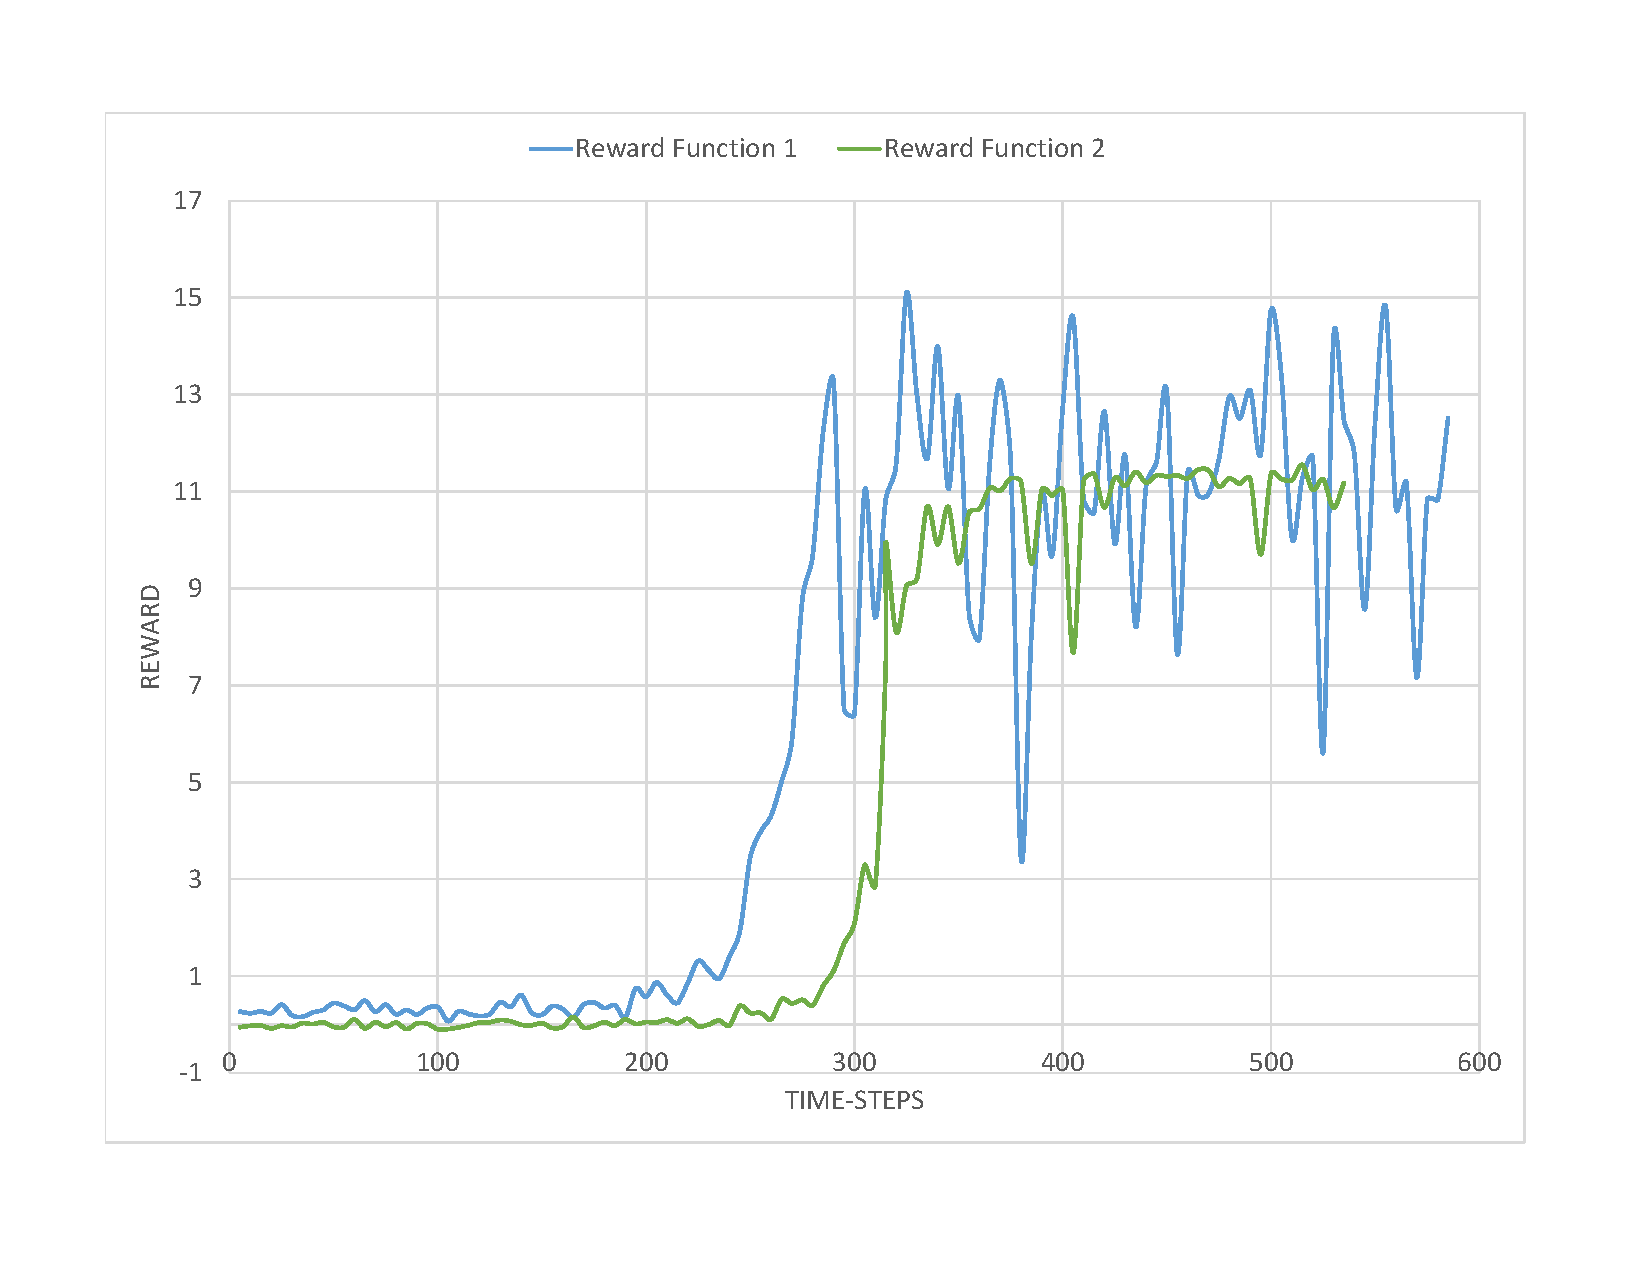
\includegraphics[width=1\textwidth]{Figures/Result/change_of_Reward_reward_graph.pdf}
	\caption{Comparison of the two different reward function with the reward getting from the environment}
	\label{fig:change_of_Reward_reward_graph}
\end{figure}

The \Cref{fig:change_of_Reward_reward_graph} shows the mean total reward of 5 time-steps (episodes). The reward after every step is added together to get the total reward. The total reward is then the reward when an episode is finish. An episode is finished when the car is out of track, the car is driving backwards or the car has finished a lap on the track.  

On the graph on \Cref{fig:change_of_Reward_reward_graph} it is seen that both reward function have the wanted effect, and the first reward function learns a bit faster than the second reward function around 250 time-steps and the second reward function learn around 320 time-steps. The negative side of the first reward function is it is not as stable as the second reward function, by looking at the graphs the second reward function is more stable than the first. 

The stability of the learning can also be seen on the car in the TORCS environment. Here it looks like the first reward function drives close to the edge of the track, and learns how to follow the red and white stripes edges. In the second reward function the car learns to drive better near the center of the road, where the car is more following the white lines in the center of the road. 

The second reward function works best, it is then the reward function which has been used in the final algorithm for the agent.  

\section{Acceleration}
The acceleration is another important parameter in this project. It became important because in the start of the project, the agent has to learn how to accelerate itself. The agent with discrete actions didn't learn the right policy with having the acceleration as an trainable parameter. Acceleration was then changed from an trainable parameter to a constant parameter.

This was done to see if it was possible for the agent to learn how to drive a lap on different speed. This was done because it could be more realistic if it is possible to see the car driving faster than 10 km/h. The tested speed was with an interval of 20 km/h:
\begin{itemize}
	\item 10 km/h
	\item 30 km/h
	\item 50 km/h
\end{itemize} 

The way the car was driving these average speed, was first the car accelerate to a speed of 30 km/h example. After this then accelerating so the speed always stays at 30 km/h. The car will try to stay at this speed 30 km/h the whole lap. To accelerate it is the throttle in the environment which need to be changed.

To test the acceleration influence on the agent learning, all other parameters is as described in the introduction to this \Cref{cha:Result}. Thereby it should be possible to only see the influence on the acceleration.

The most important graph is the graph of the reward, which looks different from all the acceleration, this graph can be seen on {ref to FIGURE reward GRAPH}.


\textbf{FIGURE reward GRAPH}  


On {ref to FIGURE reward GRAPH} it is possible to see what happens with the different accelerations.   
 

  
\section{Acceleration}\label{sectionAcceleration_new}
After many tests, and implementation it was possible to add another discrete action - the acceleration. Instead of the car driving with a constant speed as seen in \Cref{sectionAcceleration}, the agent can learn how to accelerate the car. This gives a more realistic view on the car simulation, because humans don't just drive on a constant speed all the time, sometimes it is better to drive fast, and sometimes it is better to drive slow.  

The acceleration is a discrete action, but it is a discrete action the car should learn, to be able to drive a lap. The most optimal parameter for the acceleration need to be found. The acceleration is a number between 0 and 1, where 0 means no throttle and 1 is full throttle. It is thereby the throttle in the car which decides the acceleration, and it is the throttle which is the discrete action.

The different acceleration/throttle values tested as a discrete action is:
\begin{itemize}
	\item 0.1
	\item 0.2
	\item 0.4
\end{itemize} 
   
If the acceleration is bigger the car will accelerate faster - the speed will increase faster. Because no break action is implemented, this means if the car has a bigger acceleration, the speed in general will be bigger. 

To see if the agent is able to learn how to drive, a graph of the total reward is seen on \Cref{fig:change_of_acceleration_new_reward_graph}.

\begin{figure}[H]
	\centering
	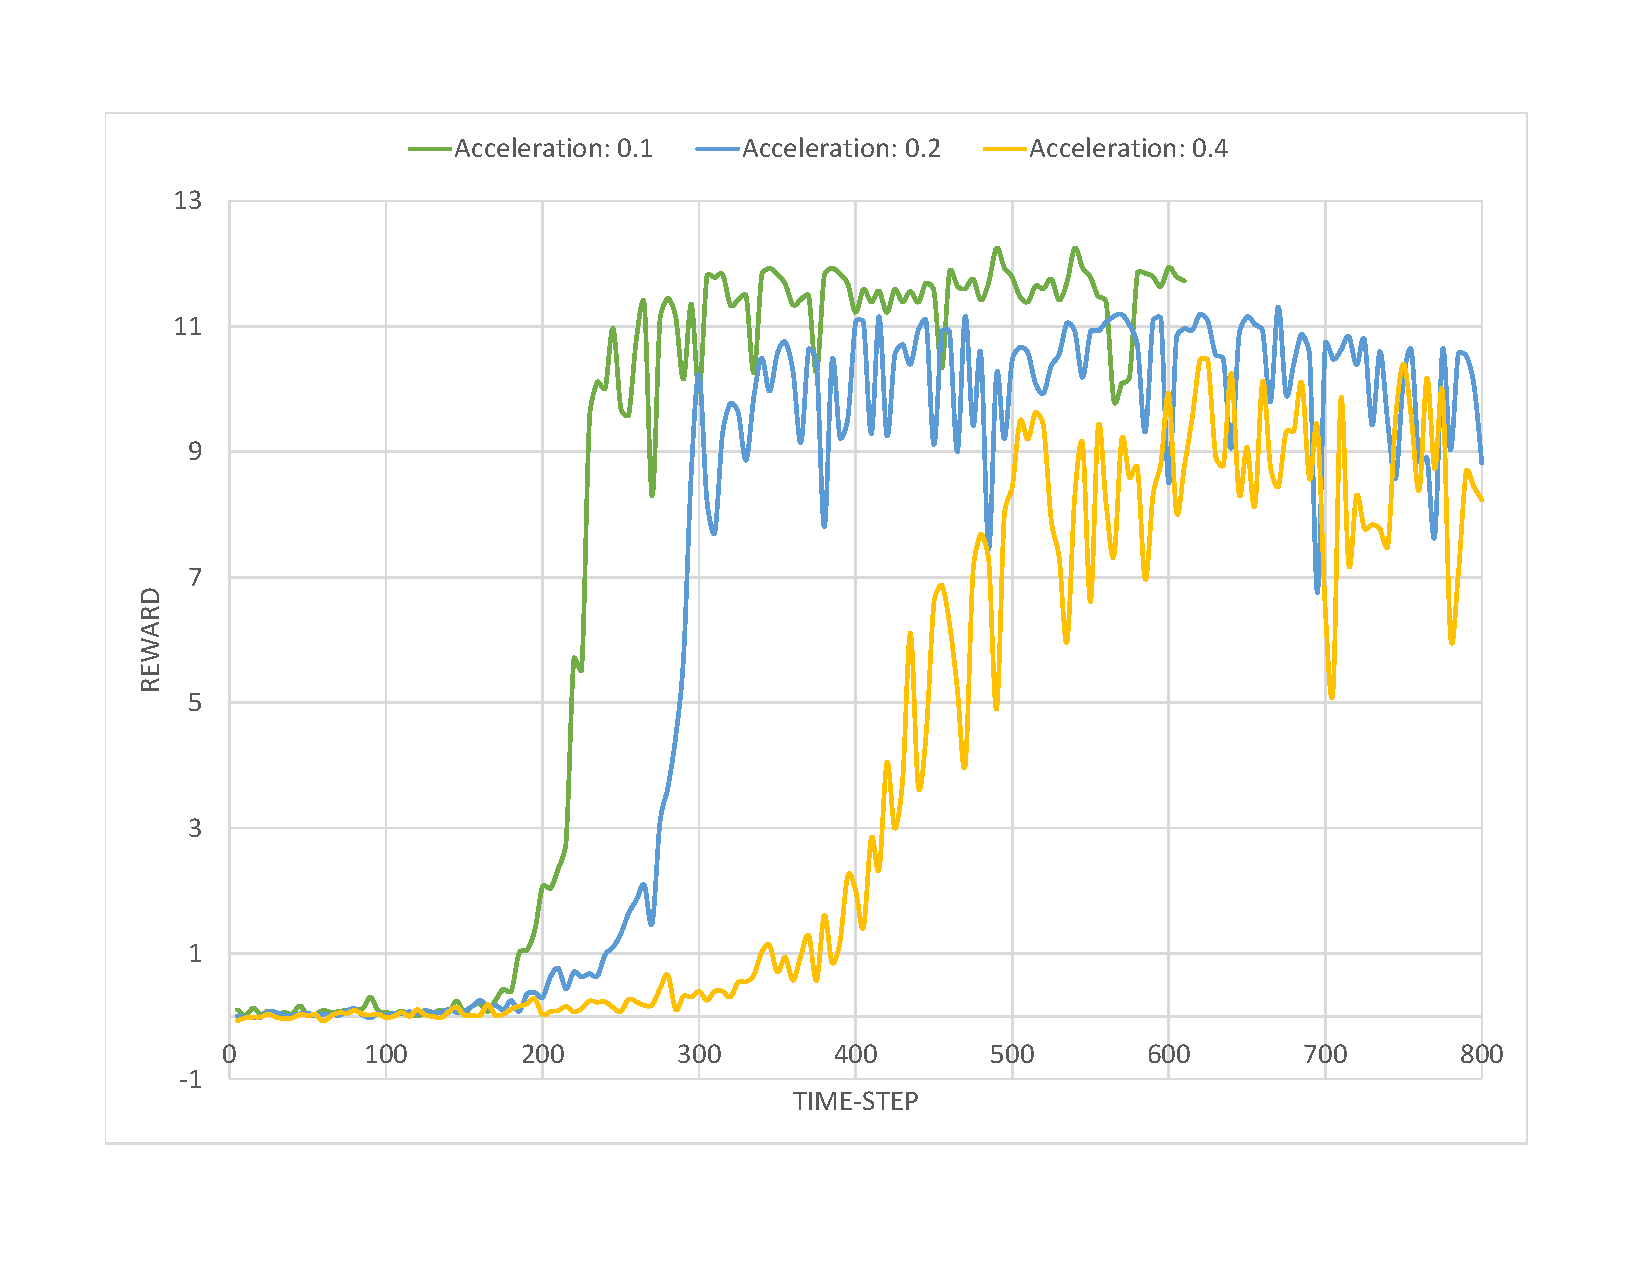
\includegraphics[width=1\textwidth]{Figures/Result/change_of_acceleration_new_reward_graph.pdf}
	\caption{Comparison of the three different acceleration with the reward getting from the environment}
	\label{fig:change_of_acceleration_new_reward_graph}
\end{figure} 

On \Cref{fig:change_of_acceleration_new_reward_graph} it is seen that all the different acceleration values converge to a reward value. In the graph, it looks like the agent has learned how to drive the car a lap. This is also the conclusion by looking at the car in the TORCS environment. 

The reward is higher with an acceleration of 0.1 than with accelerations of 0.2 or 0.4. This is since it drives slower, it uses more steps to finish the lap, and the total reward is equal to the reward in all the steps added together. This is not seen as a problem in this project, because it is only needed to learn how to drive a lap, and not to drive it fast, and all the accelerations learn how to drive a lap.

The stability is different for the different accelerations. Here it is more stable with an acceleration of 0.1 instead of 0.2 or 0.4. This can be because of the discrete value for steering as mention in \Cref{sectionAcceleration}. The discrete steering values is optimized to a speed of 10 km/h. Sometimes the speed reaches 60 km/h with an acceleration of 0.4, the steering values should then be changed.  

Looking at the training time, it looks like it is learning slower with an acceleration of 0.4 than with 0.2 and 0.1. This is the same problem with the speed in \Cref{sectionAcceleration}. With an acceleration of 0.4 the time-steps finish faster, so it takes more time-steps to learn. To get a better view of the training time, a graph with training time in hours instead of time-steps is created. This graph can be seen on \Cref{fig:change_of_acceleration_new_reward_hours_graph}.       

\begin{figure}[H]
	\centering
	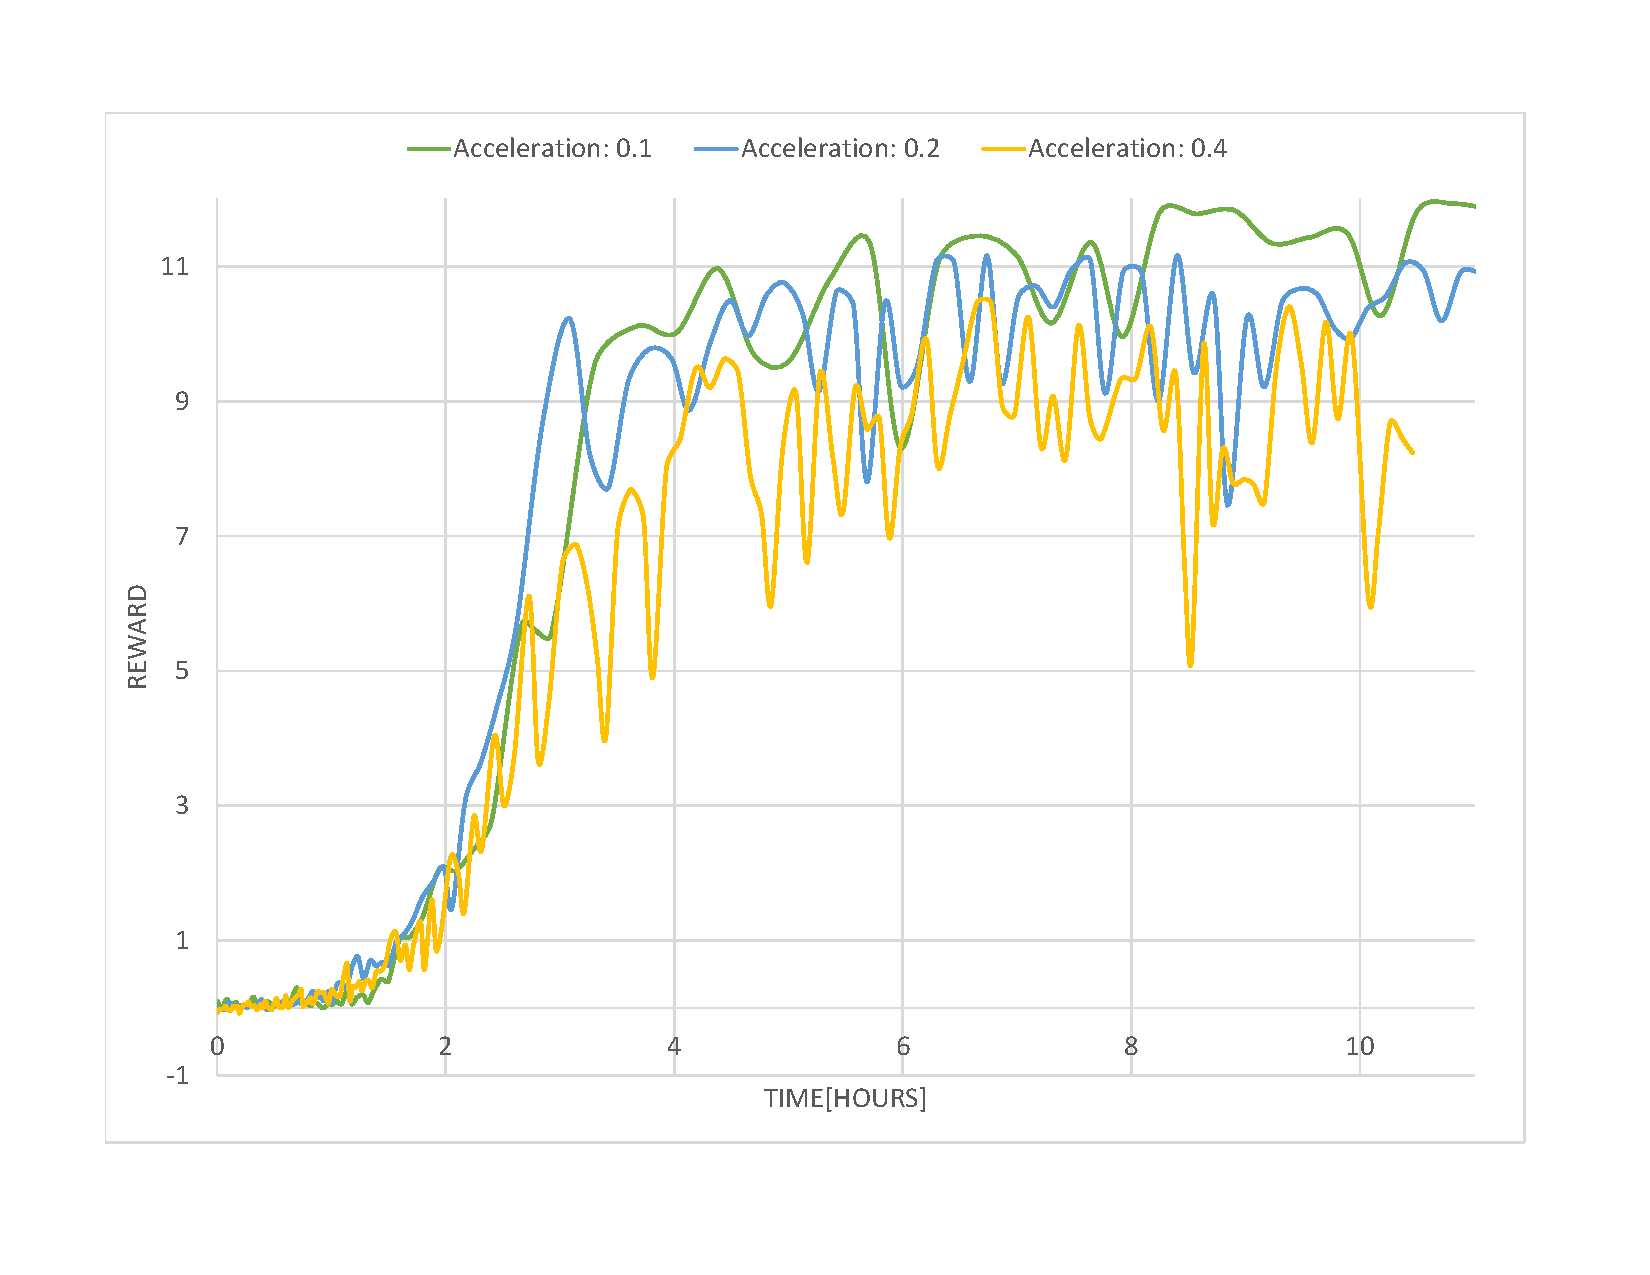
\includegraphics[width=1\textwidth]{Figures/Result/change_of_acceleration_new_reward_hours_graph.pdf}
	\caption{Comparison of the three different acceleration with the reward getting from the environment. Here it is the time in hours, instead of time-steps on the x-axis}
	\label{fig:change_of_acceleration_new_reward_hours_graph}
\end{figure}

On \Cref{fig:change_of_acceleration_new_reward_hours_graph} It is seen the training time is the same for all accelerations - around 3 hours. 

Most of the result in this \Cref{cha:Result} is done without the acceleration as an action, due to the timescale of the project, this action was implemented late in the project. If more testing should be done in the future, it is concluded that acceleration as an action would work without problems.   
\section{Tracks}\label{Tracks}
In the TORCS environment is it possible to change the tracks the car is racing in. This is done, to see how it will effect the training. The different tracks is also used for testing. It is possible to test if the car has learned how to drive, by training the car on one track, and then testing it on another track. The car should then be able to drive on both track.  

The setup to test this is the best setup as described in the introduction to this \Cref{cha:Result}. The same setup is then used in all the different track the car has been training on, this is done to make sure that the results from the different track have the same parameters on all the tracks. 

In the environment TORCS there are many different tracks. To get the agent to learn how to drive, a simple track was decided. This was done due to more complicated tracks, had more obstacles like bridges, tress and mountains. A problem with these obstacles is if the agent has to turn left for the first time and it sees many tress there. Then the agent could end up learning it has to turn left every time it sees a tree. then it will take longer for the agent to learn how to drive if there is many obstacles it has to take into account. 

Another issue seen on more complicated tracks is the road the car drives on some times changes through the track also the boundaries of the track can change. This will make it complicated from an agent to learn something, and maybe ending up not learning how to drive. The biggest issue is it will also increase the training time, which will be to long. 

The track shouldn't be to simple, it still has to look like a real road, it also need to have some turns both left and right, so it learns how to drive. 

The track which has been used mostly in this project is a simple track, which have the same road type in the whole track. The track also doesn't have obstacles, only grass around the road, and to boundary from the road to the grass is red and white stripes on the whole track. It has both left and right turns, and also just straight forward, the agent then learn all the different scenarios. The track used mostly in this project can be seen on \Cref{fig:track_simple_1}.

\begin{figure}[H]
	\centering
	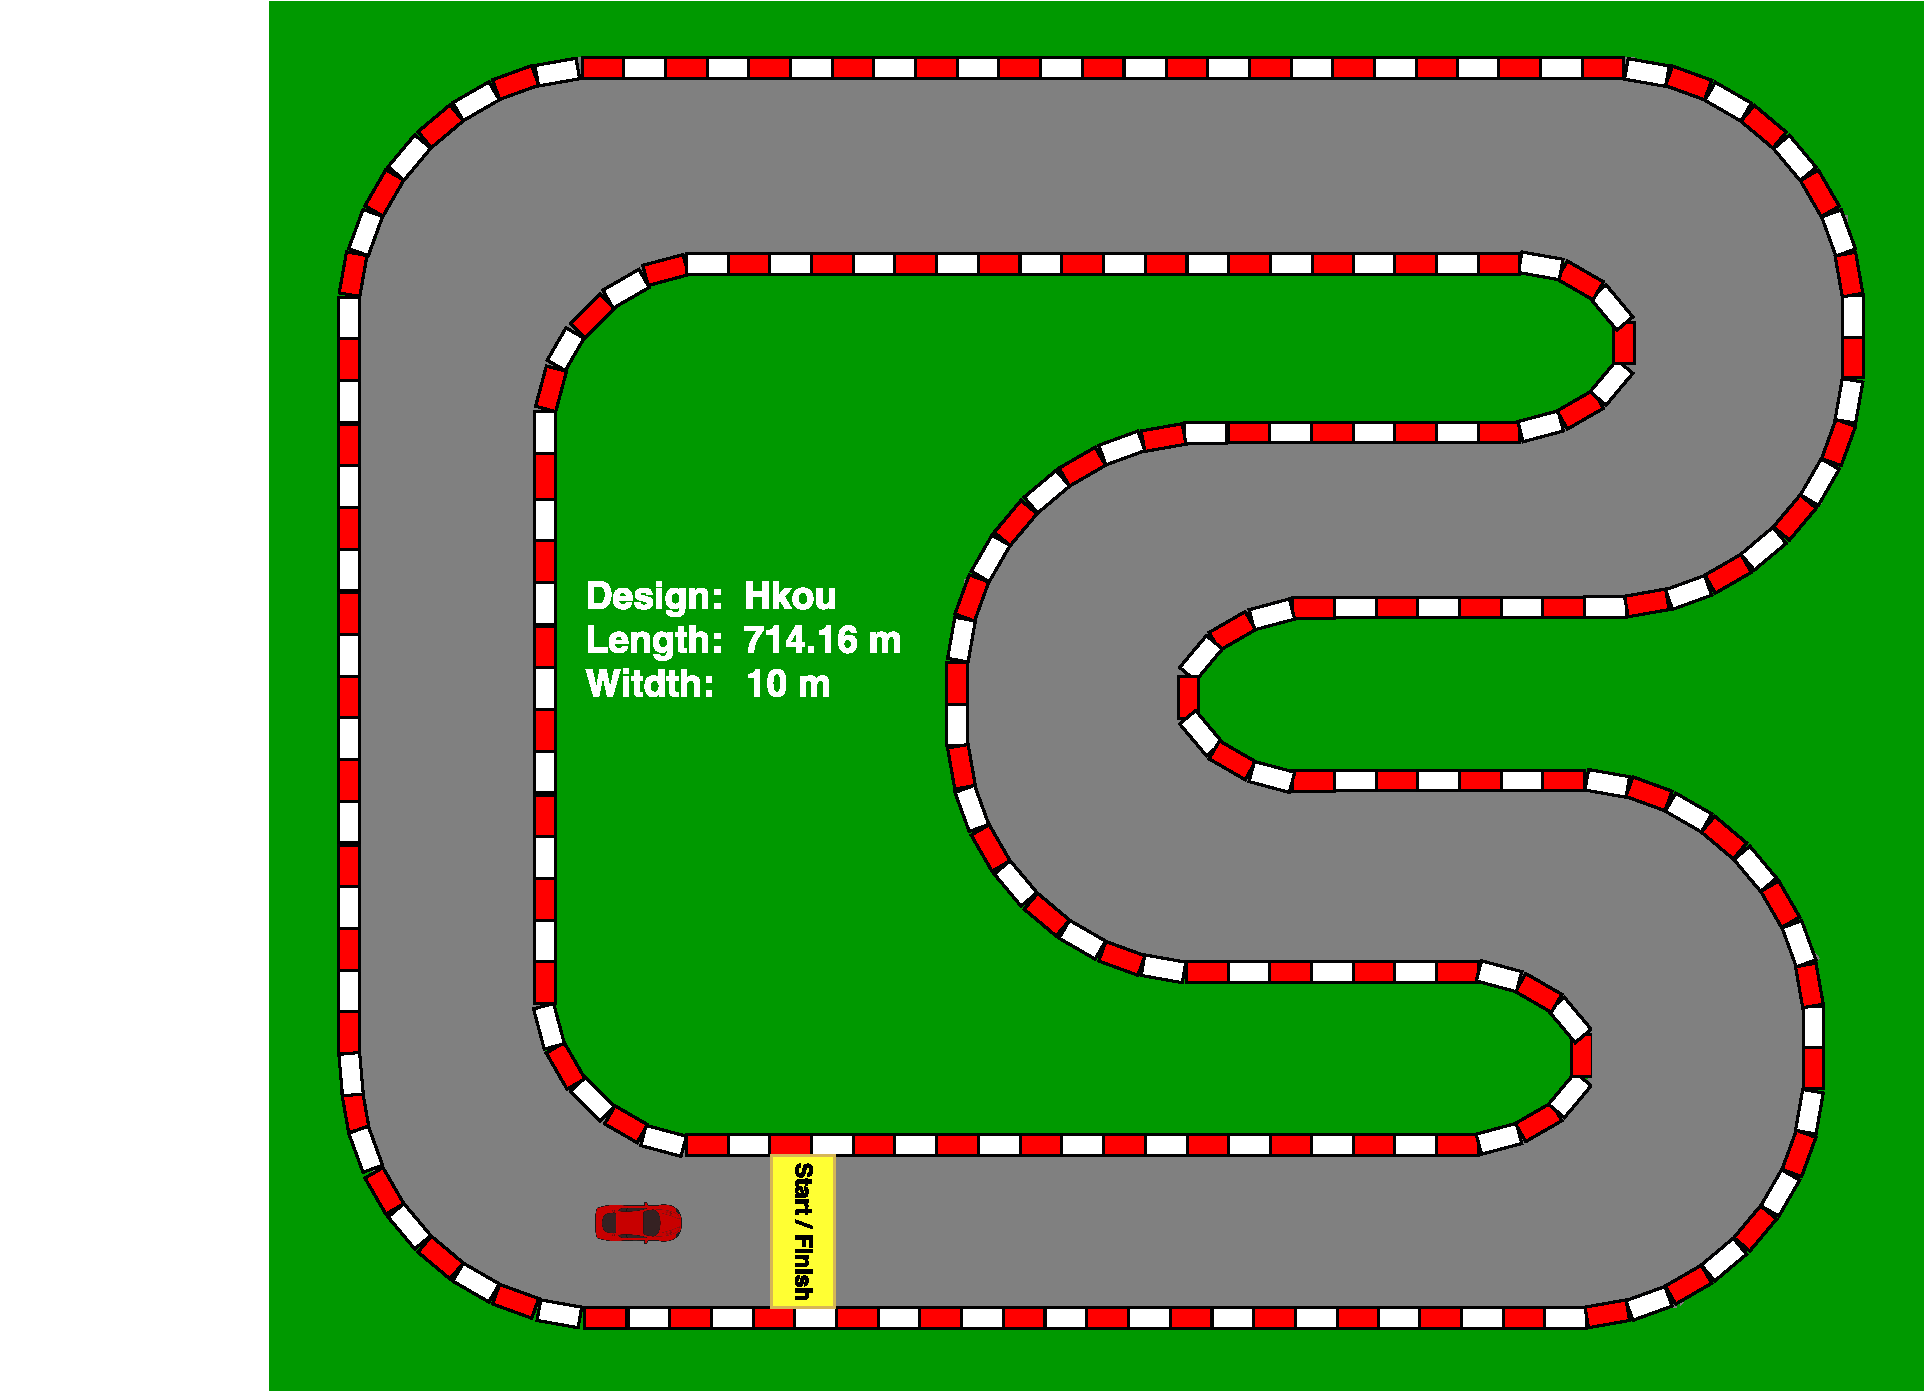
\includegraphics[width=1\textwidth]{Figures/Result/track_simple_1.pdf}
	\caption{The first track used is called $simple\_1$ made by Hkou}
	\label{fig:track_simple_1}
\end{figure}

To find other tracks to train and test on, it has to look similar to the one on \Cref{fig:track_simple_1}, because as mentioned before it learns from the input image. So if it should be possible to test the trained agent, it has to see some of the same things on the test track as on the training track. In the TORCS environment there are three tracks, which look similar the one on \Cref{fig:track_simple_1} and two others. 

The second track used in this project is a track which looks really similar to the first track, and the name is simple\_2 instead of simple\_1. The only difference from the first track is, it is mirrored. This mean that all the turns are exactly opposite. The track is thereby good for testing, because it has different turns than the first track. The second track can be seen on \Cref{fig:track_simple_2}.

\begin{figure}[H]
	\centering
	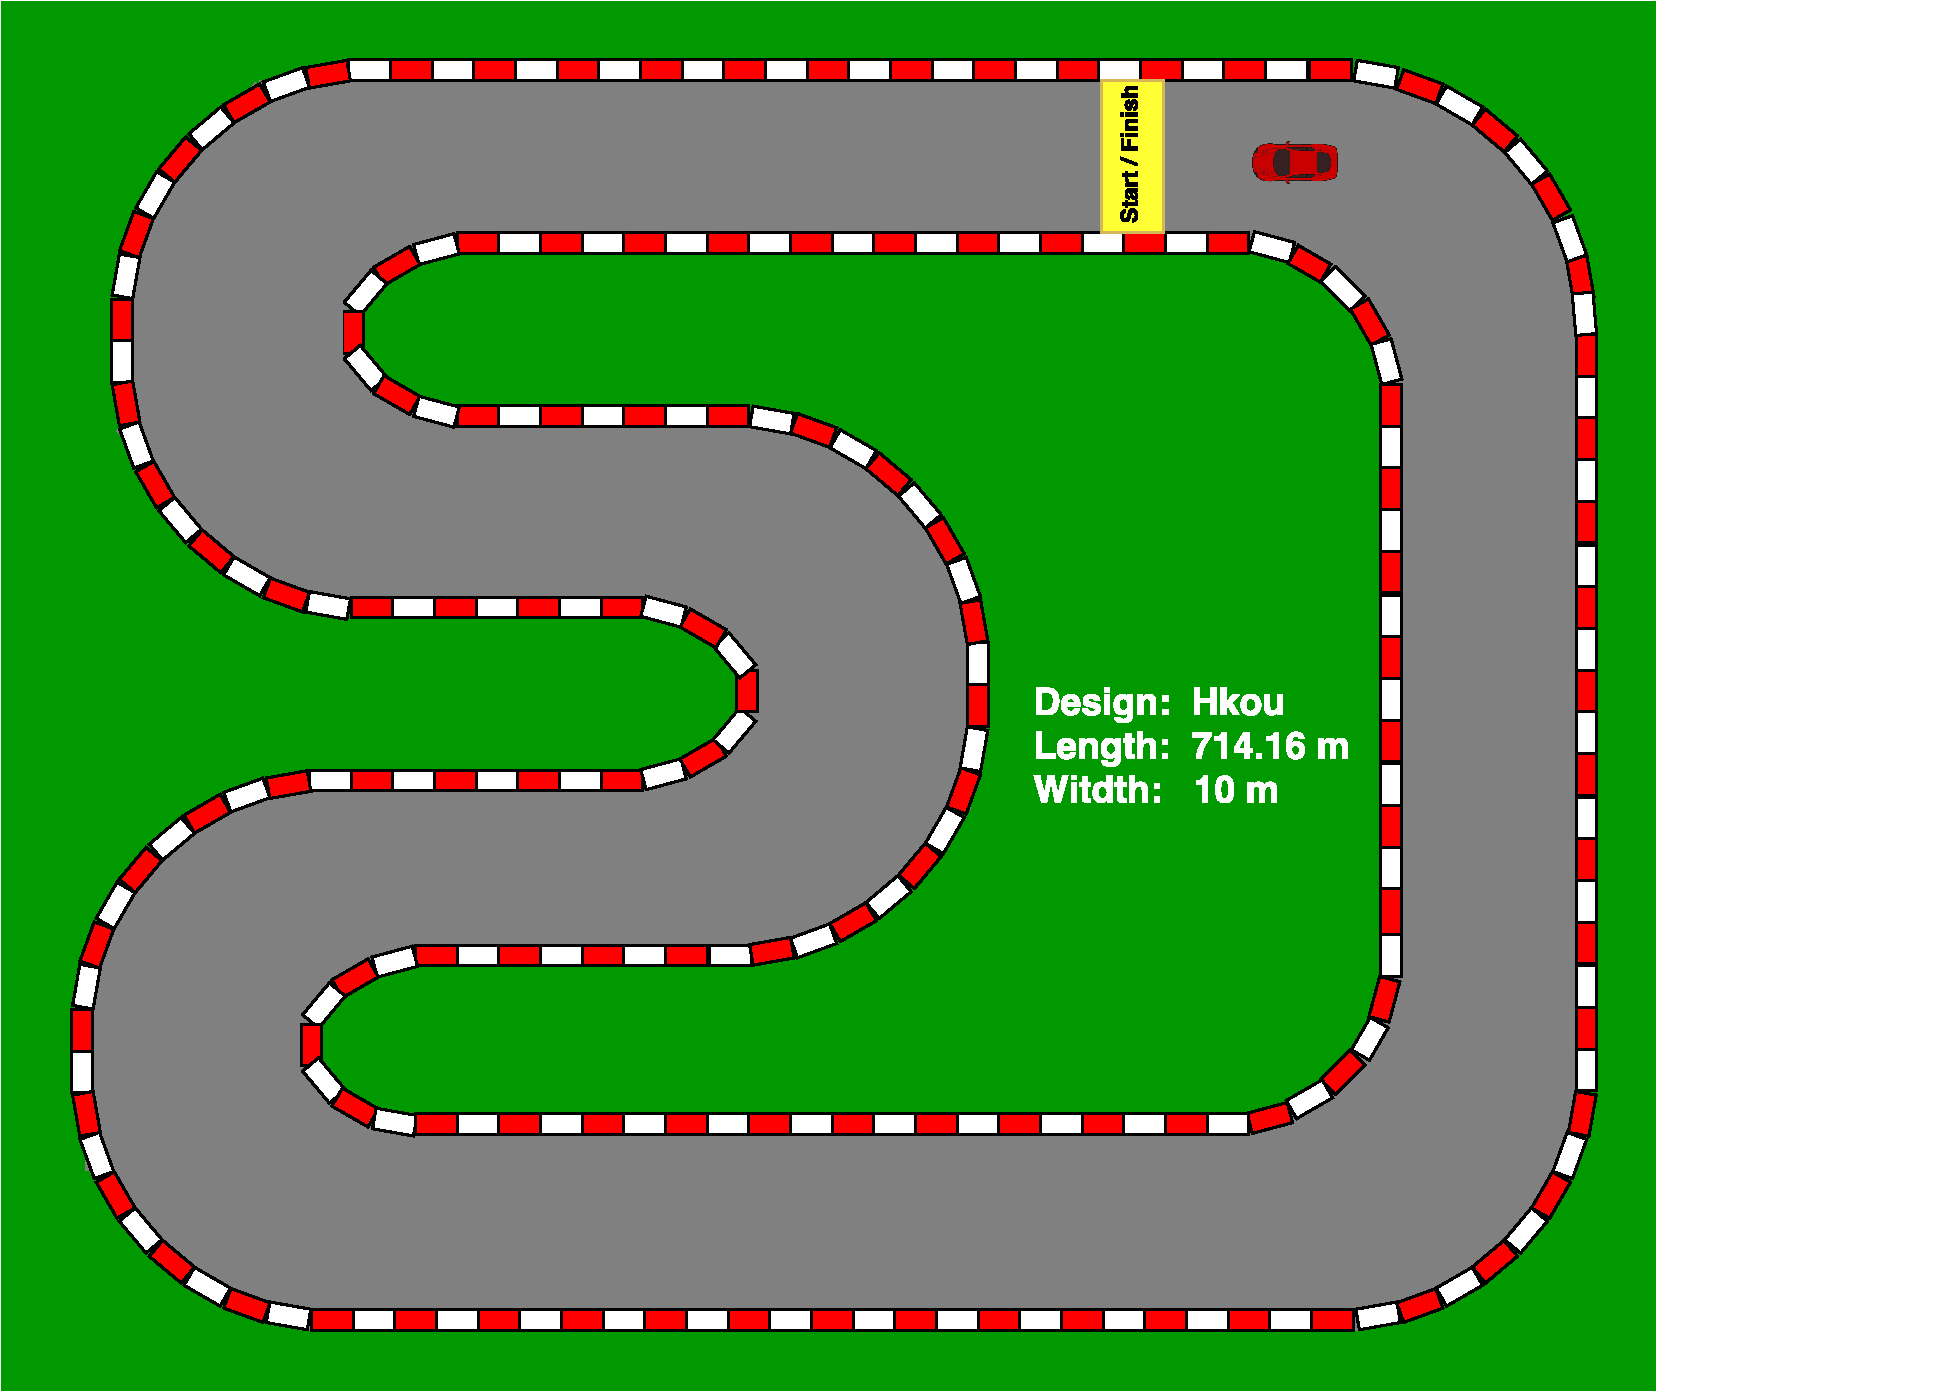
\includegraphics[width=1\textwidth]{Figures/Result/track_simple_2.pdf}
	\caption{The second track used is called $simple\_2$ made by Hkou}
	\label{fig:track_simple_2}
\end{figure}

The last track is similar to the two other tracks on \Cref{fig:track_simple_1} and \Cref{fig:track_simple_2}. The only difference is it is more simple, only has left turns. Another difference form the other two tracks is the length it is much longer than the other tracks. It is because of this length it is used to see how the agent learns on a different track with a longer distance. The last used track in this project can be seen on \Cref{fig:track_longstr}. 

\begin{figure}[H]
	\centering
	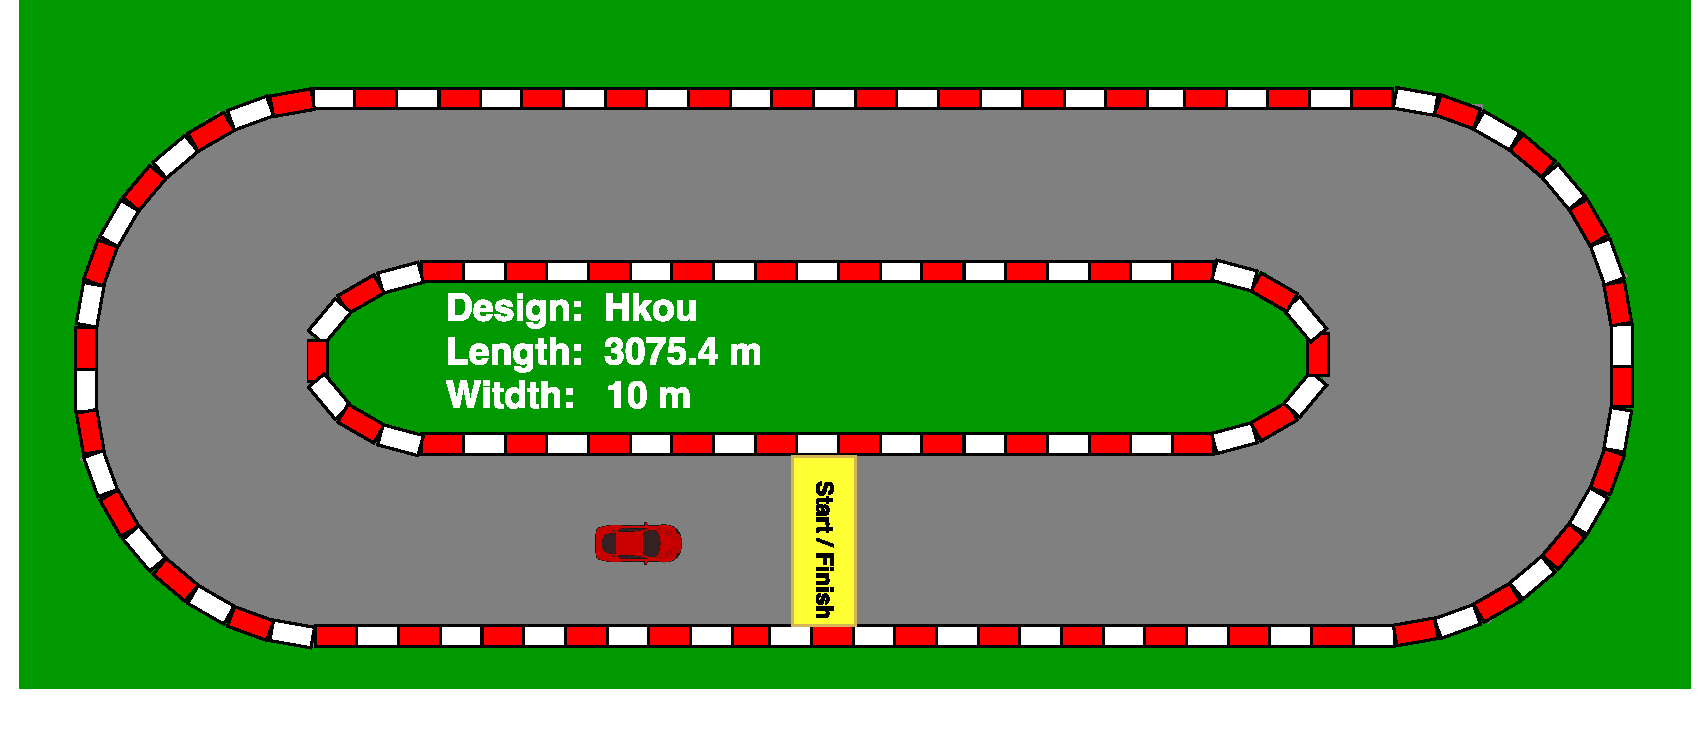
\includegraphics[width=1\textwidth]{Figures/Result/track_longstr.pdf}
	\caption{The third track used is called $longstr$ made by Hkou}
	\label{fig:track_longstr}
\end{figure}


\subsection*{Training}
In this project, it is tested if the tracks has an influence on the training. This is done to see if there is some of the used track which is better to train on than the others.

To compare this training the reward graph is used, the agent has trained on the three different tracks (\Cref{fig:track_simple_1}, \Cref{fig:track_simple_2} and \Cref{fig:track_longstr}). Here it would be better if the reward is growing faster on one of the tracks than the others, and even more important converge to the optimal reward faster. The reward graph can be seen on \Cref{fig:change_of_track_reward_graph}.

\begin{figure}[H]
	\centering
	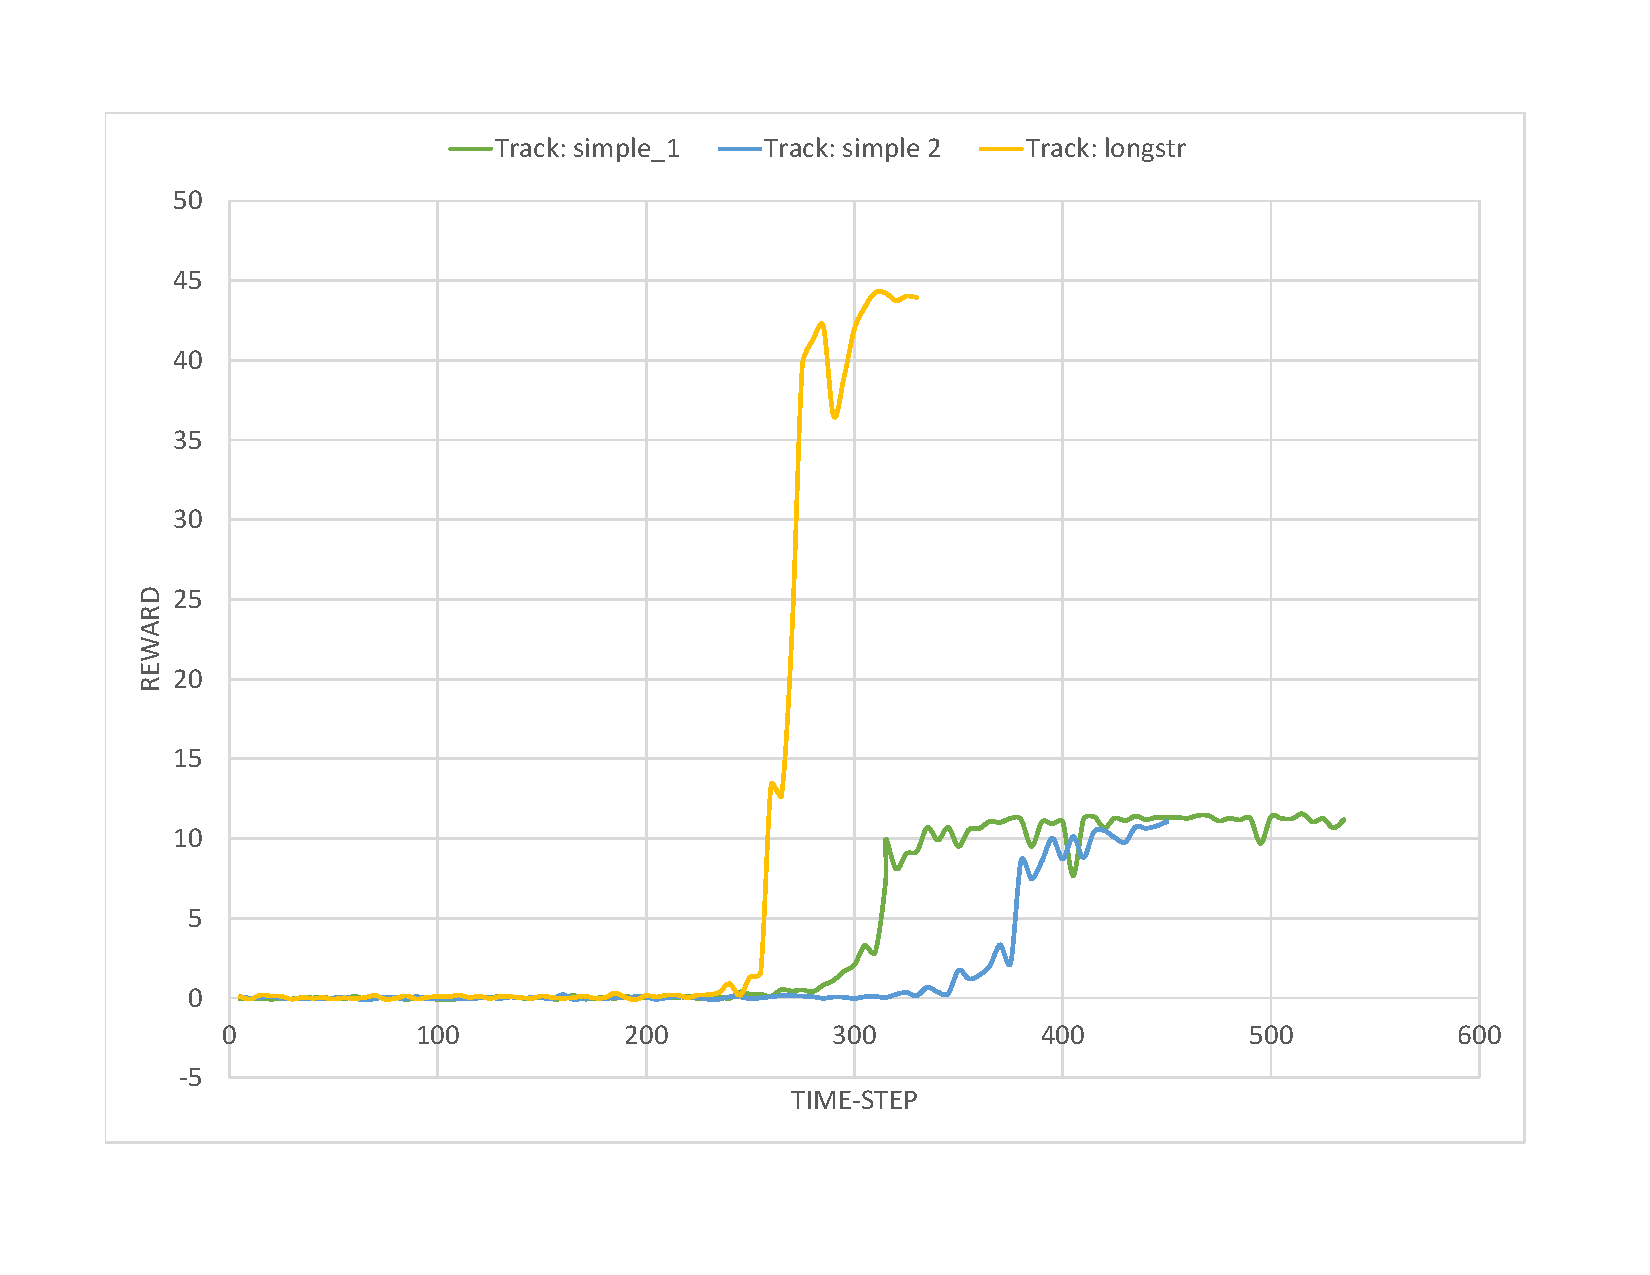
\includegraphics[width=1\textwidth]{Figures/Result/change_of_track_reward_graph.pdf}
	\caption{Comparison of the three different tracks with the reward getting from the environment}
	\label{fig:change_of_track_reward_graph}
\end{figure}

Here it is seen that the different track doesn't have any influence on when the reward starts to grow, they all start around 300 episodes. For the first two tracks which is similar, just mirrored, they have the same graphs. It is as expected, because they have the same length, reward function and acceleration, the training time and reward should then be the same. 

The difference is the reward on the third track, which can be seen to converge to a bigger reward than getting on the two other tracks. This is because of the length of the track. It can get a bigger reward, when the track is longer. This is because the length of every episode is longer. The length of the episodes on the different tracks can be seen on \Cref{fig:change_of_track_length_graph }     

\begin{figure}[H]
	\centering
	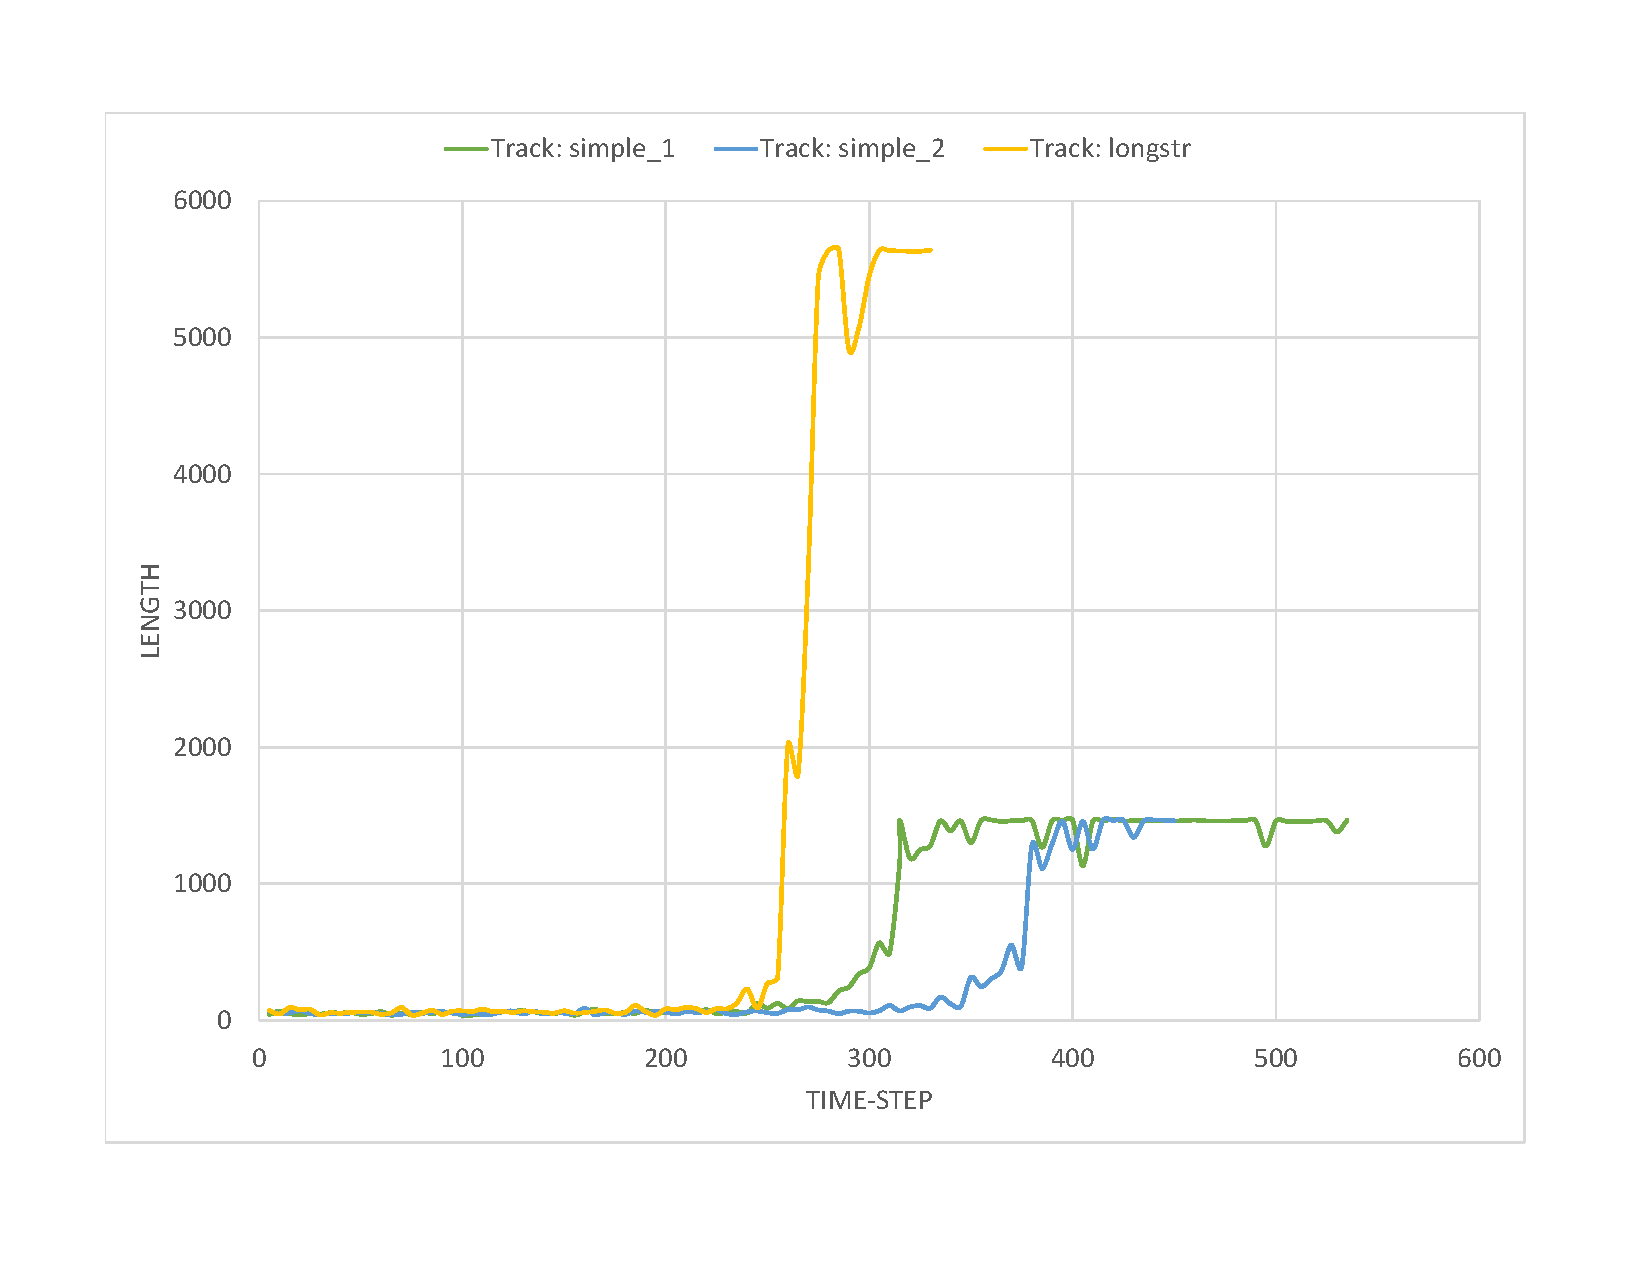
\includegraphics[width=1\textwidth]{Figures/Result/change_of_track_length_graph.pdf}
	\caption{Comparison of the three different tracks with the length of the episodes}
	\label{fig:change_of_track_length_graph}
\end{figure}

Because the track is 3-4 times bigger the reward is also 3-4 times bigger \textbf{formulas of the reward and performance}

After these result the track wich have been used in all the other trainings is the first track seen on \Cref{fig:track_simple_1}. To test if the agent has learned how to drive the second track is used seen on \Cref{fig:track_simple_2}. If the agent is able to complete a lap on both of these tracks it is concluded the agent has learned how to drive.   





\chapter{Discussion}
\chapter{Conclusion}\label{Conclusion}

%\include{Kapitler/Referencer}



%%%% References %%%%
\begingroup
\raggedright
\bibliography{References/References}							
% Litteraturlisten inkluderes
\endgroup

%%%% Fixme-list %%%%
\newpage														% New page to Fixme-list
%\listoffixmes													% Fixme-list - removes in the end with "%"

%%%% Appendix %%%%
\appendix														% Appendix start - gives chapters letters instead of numbers
\clearforchapter												% Secure that the pagestyle activates on the right page
\phantomsection													% artificial chapter that hyperlinks can  'maintain in'
\pdfbookmark[0]{Appendiks}{appendiks}							% gives the possibility to clickable bookmark for the final PDF

\end{document}													% finnish document - required